\documentclass[twoside]{book}

% Packages required by doxygen
\usepackage{fixltx2e}
\usepackage{calc}
\usepackage{doxygen}
\usepackage[export]{adjustbox} % also loads graphicx
\usepackage{graphicx}
\usepackage[utf8]{inputenc}
\usepackage{makeidx}
\usepackage{multicol}
\usepackage{multirow}
\PassOptionsToPackage{warn}{textcomp}
\usepackage{textcomp}
\usepackage[nointegrals]{wasysym}
\usepackage[table]{xcolor}

% Font selection
\usepackage[T1]{fontenc}
\usepackage[scaled=.90]{helvet}
\usepackage{courier}
\usepackage{amssymb}
\usepackage{sectsty}
\renewcommand{\familydefault}{\sfdefault}
\allsectionsfont{%
  \fontseries{bc}\selectfont%
  \color{darkgray}%
}
\renewcommand{\DoxyLabelFont}{%
  \fontseries{bc}\selectfont%
  \color{darkgray}%
}
\newcommand{\+}{\discretionary{\mbox{\scriptsize$\hookleftarrow$}}{}{}}

% Page & text layout
\usepackage{geometry}
\geometry{%
  a4paper,%
  top=2.5cm,%
  bottom=2.5cm,%
  left=2.5cm,%
  right=2.5cm%
}
\tolerance=750
\hfuzz=15pt
\hbadness=750
\setlength{\emergencystretch}{15pt}
\setlength{\parindent}{0cm}
\setlength{\parskip}{3ex plus 2ex minus 2ex}
\makeatletter
\renewcommand{\paragraph}{%
  \@startsection{paragraph}{4}{0ex}{-1.0ex}{1.0ex}{%
    \normalfont\normalsize\bfseries\SS@parafont%
  }%
}
\renewcommand{\subparagraph}{%
  \@startsection{subparagraph}{5}{0ex}{-1.0ex}{1.0ex}{%
    \normalfont\normalsize\bfseries\SS@subparafont%
  }%
}
\makeatother

% Headers & footers
\usepackage{fancyhdr}
\pagestyle{fancyplain}
\fancyhead[LE]{\fancyplain{}{\bfseries\thepage}}
\fancyhead[CE]{\fancyplain{}{}}
\fancyhead[RE]{\fancyplain{}{\bfseries\leftmark}}
\fancyhead[LO]{\fancyplain{}{\bfseries\rightmark}}
\fancyhead[CO]{\fancyplain{}{}}
\fancyhead[RO]{\fancyplain{}{\bfseries\thepage}}
\fancyfoot[LE]{\fancyplain{}{}}
\fancyfoot[CE]{\fancyplain{}{}}
\fancyfoot[RE]{\fancyplain{}{\bfseries\scriptsize Generated by Doxygen }}
\fancyfoot[LO]{\fancyplain{}{\bfseries\scriptsize Generated by Doxygen }}
\fancyfoot[CO]{\fancyplain{}{}}
\fancyfoot[RO]{\fancyplain{}{}}
\renewcommand{\footrulewidth}{0.4pt}
\renewcommand{\chaptermark}[1]{%
  \markboth{#1}{}%
}
\renewcommand{\sectionmark}[1]{%
  \markright{\thesection\ #1}%
}

% Indices & bibliography
\usepackage{natbib}
\usepackage[titles]{tocloft}
\setcounter{tocdepth}{3}
\setcounter{secnumdepth}{5}
\makeindex

% Hyperlinks (required, but should be loaded last)
\usepackage{ifpdf}
\ifpdf
  \usepackage[pdftex,pagebackref=true]{hyperref}
\else
  \usepackage[ps2pdf,pagebackref=true]{hyperref}
\fi
\hypersetup{%
  colorlinks=true,%
  linkcolor=blue,%
  citecolor=blue,%
  unicode%
}

% Custom commands
\newcommand{\clearemptydoublepage}{%
  \newpage{\pagestyle{empty}\cleardoublepage}%
}

\usepackage{caption}
\captionsetup{labelsep=space,justification=centering,font={bf},singlelinecheck=off,skip=4pt,position=top}

%===== C O N T E N T S =====

\begin{document}

% Titlepage & ToC
\hypersetup{pageanchor=false,
             bookmarksnumbered=true,
             pdfencoding=unicode
            }
\pagenumbering{alph}
\begin{titlepage}
\vspace*{7cm}
\begin{center}%
{\Large My Project }\\
\vspace*{1cm}
{\large Generated by Doxygen 1.8.14}\\
\end{center}
\end{titlepage}
\clearemptydoublepage
\pagenumbering{roman}
\tableofcontents
\clearemptydoublepage
\pagenumbering{arabic}
\hypersetup{pageanchor=true}

%--- Begin generated contents ---
\chapter{Namespace Index}
\section{Namespace List}
Here is a list of all documented namespaces with brief descriptions\+:\begin{DoxyCompactList}
\item\contentsline{section}{\mbox{\hyperlink{namespace_completed}{Completed}} }{\pageref{namespace_completed}}{}
\end{DoxyCompactList}

\chapter{Hierarchical Index}
\section{Class Hierarchy}
This inheritance list is sorted roughly, but not completely, alphabetically\+:\begin{DoxyCompactList}
\item \contentsline{section}{I\+Character}{\pageref{interface_i_character}}{}
\begin{DoxyCompactList}
\item \contentsline{section}{I\+Enemy}{\pageref{class_i_enemy}}{}
\begin{DoxyCompactList}
\item \contentsline{section}{Jack}{\pageref{class_jack}}{}
\item \contentsline{section}{Muffin\+Man}{\pageref{class_muffin_man}}{}
\end{DoxyCompactList}
\item \contentsline{section}{I\+Player}{\pageref{class_i_player}}{}
\begin{DoxyCompactList}
\item \contentsline{section}{Gingy}{\pageref{class_gingy}}{}
\item \contentsline{section}{Shadow\+Gingy}{\pageref{class_shadow_gingy}}{}
\end{DoxyCompactList}
\end{DoxyCompactList}
\item I\+Event\+System\+Handler\begin{DoxyCompactList}
\item \contentsline{section}{I\+Game\+Event\+System}{\pageref{interface_i_game_event_system}}{}
\begin{DoxyCompactList}
\item \contentsline{section}{Game\+Manager}{\pageref{class_game_manager}}{}
\end{DoxyCompactList}
\item \contentsline{section}{I\+Player}{\pageref{class_i_player}}{}
\item \contentsline{section}{I\+Test\+Event\+System}{\pageref{interface_i_test_event_system}}{}
\begin{DoxyCompactList}
\item \contentsline{section}{Enemy\+AI}{\pageref{class_enemy_a_i}}{}
\item \contentsline{section}{Test\+Manager}{\pageref{class_test_manager}}{}
\end{DoxyCompactList}
\item \contentsline{section}{Level\+Manager}{\pageref{class_level_manager}}{}
\end{DoxyCompactList}
\item \contentsline{section}{I\+Item}{\pageref{interface_i_item}}{}
\begin{DoxyCompactList}
\item \contentsline{section}{attack\+Item}{\pageref{classattack_item}}{}
\item \contentsline{section}{health\+Item}{\pageref{classhealth_item}}{}
\item \contentsline{section}{invincibility\+Item}{\pageref{classinvincibility_item}}{}
\end{DoxyCompactList}
\item Mono\+Behaviour\begin{DoxyCompactList}
\item \contentsline{section}{attack\+Item}{\pageref{classattack_item}}{}
\item \contentsline{section}{Attack\+Item\+Spawner}{\pageref{class_attack_item_spawner}}{}
\item \contentsline{section}{Camera\+Follow}{\pageref{class_camera_follow}}{}
\item \contentsline{section}{Completed.\+Level\+Generator}{\pageref{class_completed_1_1_level_generator}}{}
\item \contentsline{section}{Enemy\+AI}{\pageref{class_enemy_a_i}}{}
\item \contentsline{section}{Game\+Manager}{\pageref{class_game_manager}}{}
\item \contentsline{section}{Game\+Music}{\pageref{class_game_music}}{}
\item \contentsline{section}{Game\+Over}{\pageref{class_game_over}}{}
\item \contentsline{section}{Health\+Bar\+Script}{\pageref{class_health_bar_script}}{}
\item \contentsline{section}{health\+Item}{\pageref{classhealth_item}}{}
\item \contentsline{section}{Health\+Item\+Spawner}{\pageref{class_health_item_spawner}}{}
\item \contentsline{section}{I\+Enemy}{\pageref{class_i_enemy}}{}
\item \contentsline{section}{Input\+Name}{\pageref{class_input_name}}{}
\item \contentsline{section}{invincibility\+Item}{\pageref{classinvincibility_item}}{}
\item \contentsline{section}{Invincible\+Item\+Spawner}{\pageref{class_invincible_item_spawner}}{}
\item \contentsline{section}{I\+Player}{\pageref{class_i_player}}{}
\item \contentsline{section}{Jack\+Spawner}{\pageref{class_jack_spawner}}{}
\item \contentsline{section}{Level\+Manager}{\pageref{class_level_manager}}{}
\item \contentsline{section}{Loader}{\pageref{class_loader}}{}
\item \contentsline{section}{Main\+Menu}{\pageref{class_main_menu}}{}
\item \contentsline{section}{Map}{\pageref{class_map}}{}
\item \contentsline{section}{Menu\+Music}{\pageref{class_menu_music}}{}
\item \contentsline{section}{Moving\+Object}{\pageref{class_moving_object}}{}
\item \contentsline{section}{Muffin\+Man\+Controller}{\pageref{class_muffin_man_controller}}{}
\item \contentsline{section}{Muffin\+Man\+Spawner}{\pageref{class_muffin_man_spawner}}{}
\item \contentsline{section}{Pause\+Menu}{\pageref{class_pause_menu}}{}
\item \contentsline{section}{Player1\+Controller}{\pageref{class_player1_controller}}{}
\item \contentsline{section}{Player2\+Controller}{\pageref{class_player2_controller}}{}
\item \contentsline{section}{Player\+Selector}{\pageref{class_player_selector}}{}
\item \contentsline{section}{Test\+Level}{\pageref{class_test_level}}{}
\item \contentsline{section}{Test\+Loader}{\pageref{class_test_loader}}{}
\item \contentsline{section}{Test\+Manager}{\pageref{class_test_manager}}{}
\end{DoxyCompactList}
\end{DoxyCompactList}

\chapter{Class Index}
\section{Class List}
Here are the classes, structs, unions and interfaces with brief descriptions\+:\begin{DoxyCompactList}
\item\contentsline{section}{\mbox{\hyperlink{classattack_item}{attack\+Item}} }{\pageref{classattack_item}}{}
\item\contentsline{section}{\mbox{\hyperlink{class_attack_item_spawner}{Attack\+Item\+Spawner}} }{\pageref{class_attack_item_spawner}}{}
\item\contentsline{section}{\mbox{\hyperlink{class_camera_follow}{Camera\+Follow}} }{\pageref{class_camera_follow}}{}
\item\contentsline{section}{\mbox{\hyperlink{class_enemy_a_i}{Enemy\+AI}} }{\pageref{class_enemy_a_i}}{}
\item\contentsline{section}{\mbox{\hyperlink{class_game_manager}{Game\+Manager}} }{\pageref{class_game_manager}}{}
\item\contentsline{section}{\mbox{\hyperlink{class_game_music}{Game\+Music}} }{\pageref{class_game_music}}{}
\item\contentsline{section}{\mbox{\hyperlink{class_game_over}{Game\+Over}} }{\pageref{class_game_over}}{}
\item\contentsline{section}{\mbox{\hyperlink{class_gingy}{Gingy}} }{\pageref{class_gingy}}{}
\item\contentsline{section}{\mbox{\hyperlink{class_health_bar_script}{Health\+Bar\+Script}} }{\pageref{class_health_bar_script}}{}
\item\contentsline{section}{\mbox{\hyperlink{classhealth_item}{health\+Item}} }{\pageref{classhealth_item}}{}
\item\contentsline{section}{\mbox{\hyperlink{class_health_item_spawner}{Health\+Item\+Spawner}} }{\pageref{class_health_item_spawner}}{}
\item\contentsline{section}{\mbox{\hyperlink{interface_i_character}{I\+Character}} }{\pageref{interface_i_character}}{}
\item\contentsline{section}{\mbox{\hyperlink{class_i_enemy}{I\+Enemy}} }{\pageref{class_i_enemy}}{}
\item\contentsline{section}{\mbox{\hyperlink{interface_i_game_event_system}{I\+Game\+Event\+System}} }{\pageref{interface_i_game_event_system}}{}
\item\contentsline{section}{\mbox{\hyperlink{interface_i_item}{I\+Item}} }{\pageref{interface_i_item}}{}
\item\contentsline{section}{\mbox{\hyperlink{class_input_name}{Input\+Name}} }{\pageref{class_input_name}}{}
\item\contentsline{section}{\mbox{\hyperlink{classinvincibility_item}{invincibility\+Item}} }{\pageref{classinvincibility_item}}{}
\item\contentsline{section}{\mbox{\hyperlink{class_invincible_item_spawner}{Invincible\+Item\+Spawner}} }{\pageref{class_invincible_item_spawner}}{}
\item\contentsline{section}{\mbox{\hyperlink{class_i_player}{I\+Player}} }{\pageref{class_i_player}}{}
\item\contentsline{section}{\mbox{\hyperlink{interface_i_test_event_system}{I\+Test\+Event\+System}} }{\pageref{interface_i_test_event_system}}{}
\item\contentsline{section}{\mbox{\hyperlink{class_jack}{Jack}} }{\pageref{class_jack}}{}
\item\contentsline{section}{\mbox{\hyperlink{class_jack_spawner}{Jack\+Spawner}} }{\pageref{class_jack_spawner}}{}
\item\contentsline{section}{\mbox{\hyperlink{class_completed_1_1_level_generator}{Completed.\+Level\+Generator}} }{\pageref{class_completed_1_1_level_generator}}{}
\item\contentsline{section}{\mbox{\hyperlink{class_level_manager}{Level\+Manager}} }{\pageref{class_level_manager}}{}
\item\contentsline{section}{\mbox{\hyperlink{class_loader}{Loader}} }{\pageref{class_loader}}{}
\item\contentsline{section}{\mbox{\hyperlink{class_main_menu}{Main\+Menu}} }{\pageref{class_main_menu}}{}
\item\contentsline{section}{\mbox{\hyperlink{class_map}{Map}} }{\pageref{class_map}}{}
\item\contentsline{section}{\mbox{\hyperlink{class_menu_music}{Menu\+Music}} }{\pageref{class_menu_music}}{}
\item\contentsline{section}{\mbox{\hyperlink{class_moving_object}{Moving\+Object}} }{\pageref{class_moving_object}}{}
\item\contentsline{section}{\mbox{\hyperlink{class_muffin_man}{Muffin\+Man}} }{\pageref{class_muffin_man}}{}
\item\contentsline{section}{\mbox{\hyperlink{class_muffin_man_controller}{Muffin\+Man\+Controller}} }{\pageref{class_muffin_man_controller}}{}
\item\contentsline{section}{\mbox{\hyperlink{class_muffin_man_spawner}{Muffin\+Man\+Spawner}} }{\pageref{class_muffin_man_spawner}}{}
\item\contentsline{section}{\mbox{\hyperlink{class_pause_menu}{Pause\+Menu}} }{\pageref{class_pause_menu}}{}
\item\contentsline{section}{\mbox{\hyperlink{class_player1_controller}{Player1\+Controller}} }{\pageref{class_player1_controller}}{}
\item\contentsline{section}{\mbox{\hyperlink{class_player2_controller}{Player2\+Controller}} }{\pageref{class_player2_controller}}{}
\item\contentsline{section}{\mbox{\hyperlink{class_player_selector}{Player\+Selector}} }{\pageref{class_player_selector}}{}
\item\contentsline{section}{\mbox{\hyperlink{class_shadow_gingy}{Shadow\+Gingy}} }{\pageref{class_shadow_gingy}}{}
\item\contentsline{section}{\mbox{\hyperlink{class_test_level}{Test\+Level}} }{\pageref{class_test_level}}{}
\item\contentsline{section}{\mbox{\hyperlink{class_test_loader}{Test\+Loader}} }{\pageref{class_test_loader}}{}
\item\contentsline{section}{\mbox{\hyperlink{class_test_manager}{Test\+Manager}} }{\pageref{class_test_manager}}{}
\end{DoxyCompactList}

\chapter{Namespace Documentation}
\hypertarget{namespace_completed}{}\section{Completed Namespace Reference}
\label{namespace_completed}\index{Completed@{Completed}}
\subsection*{Classes}
\begin{DoxyCompactItemize}
\item 
class \mbox{\hyperlink{class_completed_1_1_level_generator}{Level\+Generator}}
\end{DoxyCompactItemize}

\chapter{Class Documentation}
\hypertarget{classattack_item}{}\section{attack\+Item Class Reference}
\label{classattack_item}\index{attack\+Item@{attack\+Item}}
Inheritance diagram for attack\+Item\+:\begin{figure}[H]
\begin{center}
\leavevmode
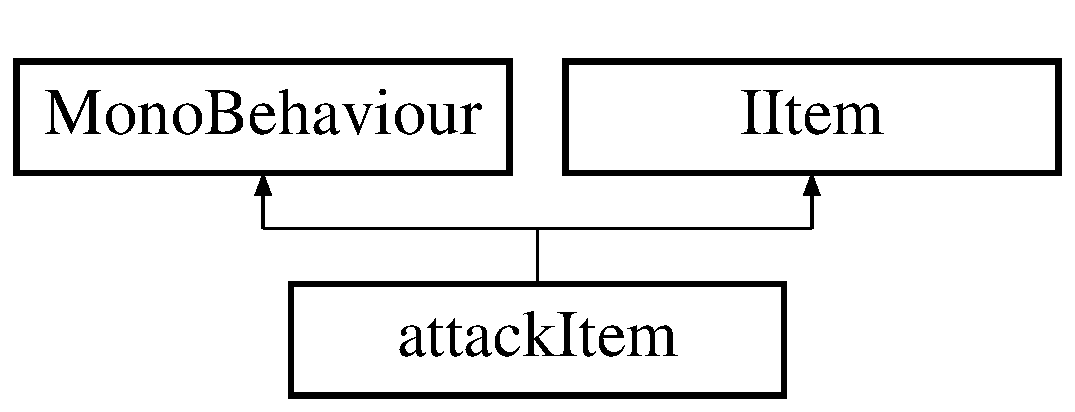
\includegraphics[height=2.000000cm]{classattack_item}
\end{center}
\end{figure}
\subsection*{Public Member Functions}
\begin{DoxyCompactItemize}
\item 
void \mbox{\hyperlink{classattack_item_ab5739e198a4a255f81d371df77bb770b}{Ability}} (\mbox{\hyperlink{class_i_player}{I\+Player}} player)
\item 
void \mbox{\hyperlink{classattack_item_a5cf5ac415471d294a3244988466d54ac}{Duration}} (\mbox{\hyperlink{class_i_player}{I\+Player}} player)
\item 
void \mbox{\hyperlink{classattack_item_ac4ed86e9328a04f08568bd9374685a15}{change\+Attack}} (\mbox{\hyperlink{class_i_player}{I\+Player}} player)
\end{DoxyCompactItemize}


\subsection{Member Function Documentation}
\mbox{\Hypertarget{classattack_item_ab5739e198a4a255f81d371df77bb770b}\label{classattack_item_ab5739e198a4a255f81d371df77bb770b}} 
\index{attack\+Item@{attack\+Item}!Ability@{Ability}}
\index{Ability@{Ability}!attack\+Item@{attack\+Item}}
\subsubsection{\texorpdfstring{Ability()}{Ability()}}
{\footnotesize\ttfamily void attack\+Item.\+Ability (\begin{DoxyParamCaption}\item[{\mbox{\hyperlink{class_i_player}{I\+Player}}}]{player }\end{DoxyParamCaption})\hspace{0.3cm}{\ttfamily [inline]}}


\begin{DoxyParams}{Parameters}
{\em \mbox{\hyperlink{class_i_player}{I\+Player}}} & \\
\hline
\end{DoxyParams}
\begin{DoxyReturn}{Returns}
none Calls the ability of the item 
\end{DoxyReturn}


Implements \mbox{\hyperlink{interface_i_item_afe73efbf8316273df20162d6f4b20648}{I\+Item}}.

\mbox{\Hypertarget{classattack_item_ac4ed86e9328a04f08568bd9374685a15}\label{classattack_item_ac4ed86e9328a04f08568bd9374685a15}} 
\index{attack\+Item@{attack\+Item}!change\+Attack@{change\+Attack}}
\index{change\+Attack@{change\+Attack}!attack\+Item@{attack\+Item}}
\subsubsection{\texorpdfstring{change\+Attack()}{changeAttack()}}
{\footnotesize\ttfamily void attack\+Item.\+change\+Attack (\begin{DoxyParamCaption}\item[{\mbox{\hyperlink{class_i_player}{I\+Player}}}]{player }\end{DoxyParamCaption})\hspace{0.3cm}{\ttfamily [inline]}}


\begin{DoxyParams}{Parameters}
{\em \mbox{\hyperlink{class_i_player}{I\+Player}}} & \\
\hline
\end{DoxyParams}
\begin{DoxyReturn}{Returns}
none Changes player\textquotesingle{}s attack stat 
\end{DoxyReturn}
\mbox{\Hypertarget{classattack_item_a5cf5ac415471d294a3244988466d54ac}\label{classattack_item_a5cf5ac415471d294a3244988466d54ac}} 
\index{attack\+Item@{attack\+Item}!Duration@{Duration}}
\index{Duration@{Duration}!attack\+Item@{attack\+Item}}
\subsubsection{\texorpdfstring{Duration()}{Duration()}}
{\footnotesize\ttfamily void attack\+Item.\+Duration (\begin{DoxyParamCaption}\item[{\mbox{\hyperlink{class_i_player}{I\+Player}}}]{player }\end{DoxyParamCaption})\hspace{0.3cm}{\ttfamily [inline]}}


\begin{DoxyParams}{Parameters}
{\em \mbox{\hyperlink{class_i_player}{I\+Player}}} & \\
\hline
\end{DoxyParams}
\begin{DoxyReturn}{Returns}
none Sets the duration of the ability 
\end{DoxyReturn}


Implements \mbox{\hyperlink{interface_i_item_a797c1d62a7828bf428cc486ceaf18e9c}{I\+Item}}.



The documentation for this class was generated from the following file\+:\begin{DoxyCompactItemize}
\item 
attack\+Item.\+cs\end{DoxyCompactItemize}

\hypertarget{class_attack_item_spawner}{}\section{Attack\+Item\+Spawner Class Reference}
\label{class_attack_item_spawner}\index{Attack\+Item\+Spawner@{Attack\+Item\+Spawner}}
Inheritance diagram for Attack\+Item\+Spawner\+:\begin{figure}[H]
\begin{center}
\leavevmode
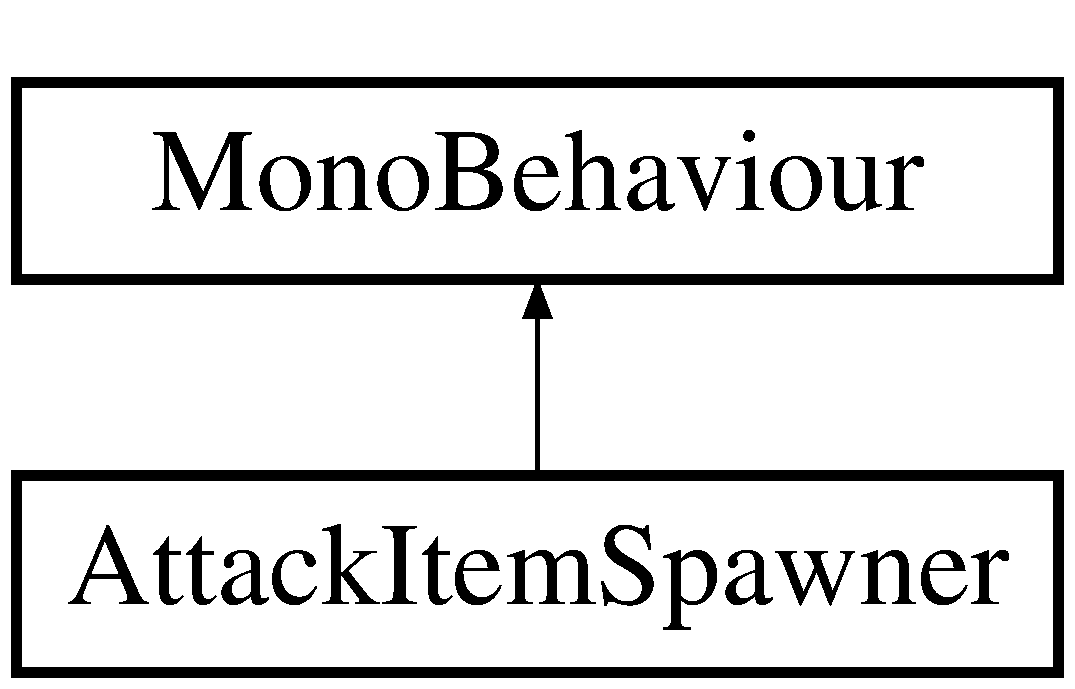
\includegraphics[height=2.000000cm]{class_attack_item_spawner}
\end{center}
\end{figure}
\subsection*{Public Attributes}
\begin{DoxyCompactItemize}
\item 
\mbox{\Hypertarget{class_attack_item_spawner_a253acf52e39449ad655b3cfba7cc111d}\label{class_attack_item_spawner_a253acf52e39449ad655b3cfba7cc111d}} 
Game\+Object {\bfseries attack\+Item}
\end{DoxyCompactItemize}


The documentation for this class was generated from the following file\+:\begin{DoxyCompactItemize}
\item 
Attack\+Item\+Spawner.\+cs\end{DoxyCompactItemize}

\hypertarget{class_camera_follow}{}\section{Camera\+Follow Class Reference}
\label{class_camera_follow}\index{Camera\+Follow@{Camera\+Follow}}
Inheritance diagram for Camera\+Follow\+:\begin{figure}[H]
\begin{center}
\leavevmode
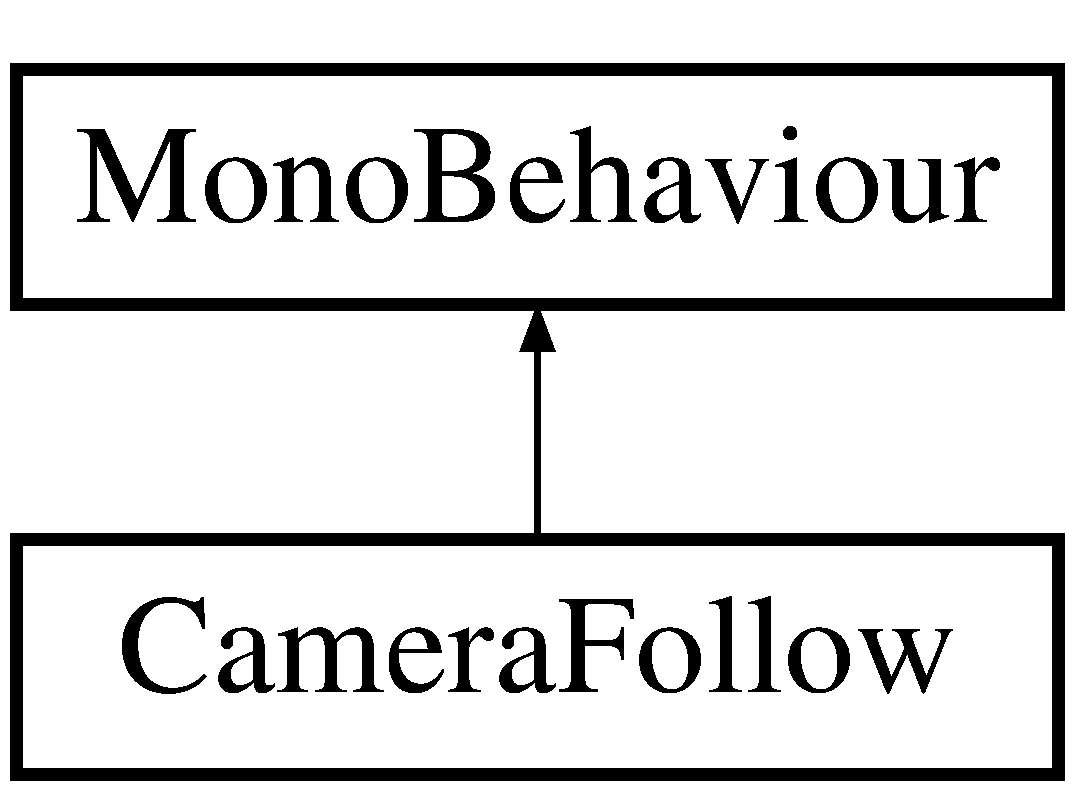
\includegraphics[height=2.000000cm]{class_camera_follow}
\end{center}
\end{figure}
\subsection*{Public Attributes}
\begin{DoxyCompactItemize}
\item 
\mbox{\Hypertarget{class_camera_follow_a2ef2d3655fd0cb86d18e6324b75c0a59}\label{class_camera_follow_a2ef2d3655fd0cb86d18e6324b75c0a59}} 
Transform {\bfseries target}
\item 
\mbox{\Hypertarget{class_camera_follow_a924c2f26a261004c89aa63ca0c89d454}\label{class_camera_follow_a924c2f26a261004c89aa63ca0c89d454}} 
float {\bfseries smooth\+Speed} = 0.\+125f
\end{DoxyCompactItemize}


The documentation for this class was generated from the following file\+:\begin{DoxyCompactItemize}
\item 
Camera\+Follow.\+cs\end{DoxyCompactItemize}

\hypertarget{class_enemy_a_i}{}\section{Enemy\+AI Class Reference}
\label{class_enemy_a_i}\index{Enemy\+AI@{Enemy\+AI}}
Inheritance diagram for Enemy\+AI\+:\begin{figure}[H]
\begin{center}
\leavevmode
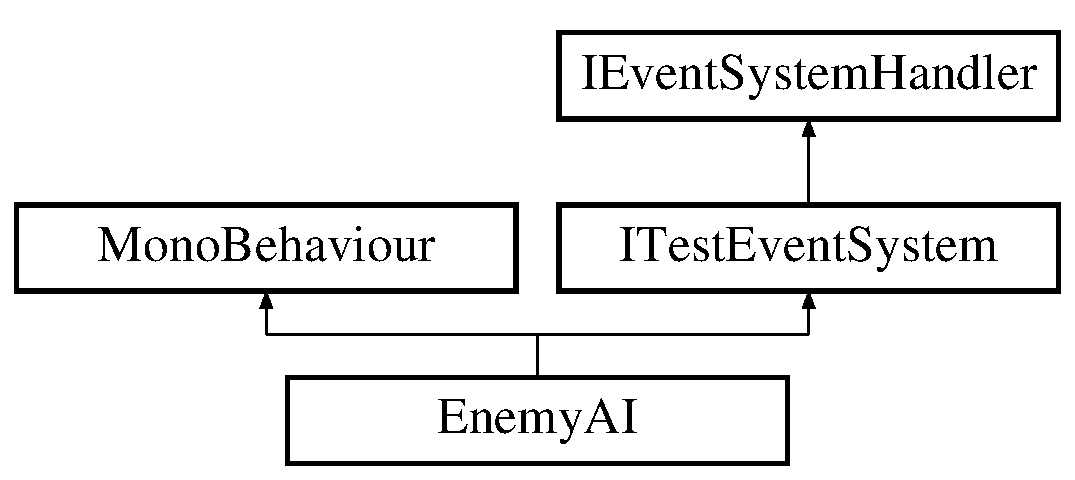
\includegraphics[height=3.000000cm]{class_enemy_a_i}
\end{center}
\end{figure}
\subsection*{Public Member Functions}
\begin{DoxyCompactItemize}
\item 
void \mbox{\hyperlink{class_enemy_a_i_a9c377a8c65147355decf5f02cf2785ea}{Try\+Attack}} ()
\item 
void \mbox{\hyperlink{class_enemy_a_i_a8d23dd153a4f273abaae5c174d10a6d2}{Start\+Test}} ()
\item 
void \mbox{\hyperlink{class_enemy_a_i_a63dc8e816322f34ec0360a1189fb931e}{End\+Test}} ()
\end{DoxyCompactItemize}
\subsection*{Public Attributes}
\begin{DoxyCompactItemize}
\item 
\mbox{\Hypertarget{class_enemy_a_i_a415f57823bb4f2490f98bedb56ae6b49}\label{class_enemy_a_i_a415f57823bb4f2490f98bedb56ae6b49}} 
Game\+Object {\bfseries Player}
\item 
\mbox{\Hypertarget{class_enemy_a_i_a207b39ab95bee140d8808cd92f966891}\label{class_enemy_a_i_a207b39ab95bee140d8808cd92f966891}} 
string {\bfseries enemy\+Name}
\end{DoxyCompactItemize}


\subsection{Member Function Documentation}
\mbox{\Hypertarget{class_enemy_a_i_a63dc8e816322f34ec0360a1189fb931e}\label{class_enemy_a_i_a63dc8e816322f34ec0360a1189fb931e}} 
\index{Enemy\+AI@{Enemy\+AI}!End\+Test@{End\+Test}}
\index{End\+Test@{End\+Test}!Enemy\+AI@{Enemy\+AI}}
\subsubsection{\texorpdfstring{End\+Test()}{EndTest()}}
{\footnotesize\ttfamily void Enemy\+A\+I.\+End\+Test (\begin{DoxyParamCaption}{ }\end{DoxyParamCaption})\hspace{0.3cm}{\ttfamily [inline]}}

End\+Test 
\begin{DoxyParams}{Parameters}
{\em none} & \\
\hline
\end{DoxyParams}
\begin{DoxyReturn}{Returns}
none Called by Event\+System\+Handler from \mbox{\hyperlink{interface_i_test_event_system}{I\+Test\+Event\+System}} 
\end{DoxyReturn}


Implements \mbox{\hyperlink{interface_i_test_event_system_ae8eda94179d81c4c839a32432216df7b}{I\+Test\+Event\+System}}.

\mbox{\Hypertarget{class_enemy_a_i_a8d23dd153a4f273abaae5c174d10a6d2}\label{class_enemy_a_i_a8d23dd153a4f273abaae5c174d10a6d2}} 
\index{Enemy\+AI@{Enemy\+AI}!Start\+Test@{Start\+Test}}
\index{Start\+Test@{Start\+Test}!Enemy\+AI@{Enemy\+AI}}
\subsubsection{\texorpdfstring{Start\+Test()}{StartTest()}}
{\footnotesize\ttfamily void Enemy\+A\+I.\+Start\+Test (\begin{DoxyParamCaption}{ }\end{DoxyParamCaption})\hspace{0.3cm}{\ttfamily [inline]}}

Start\+Test 
\begin{DoxyParams}{Parameters}
{\em none} & \\
\hline
\end{DoxyParams}
\begin{DoxyReturn}{Returns}
none Called by Event\+System\+Handler from \mbox{\hyperlink{interface_i_test_event_system}{I\+Test\+Event\+System}} 
\end{DoxyReturn}


Implements \mbox{\hyperlink{interface_i_test_event_system_aefeb7857cc94ecb2bacb47975f6474bb}{I\+Test\+Event\+System}}.

\mbox{\Hypertarget{class_enemy_a_i_a9c377a8c65147355decf5f02cf2785ea}\label{class_enemy_a_i_a9c377a8c65147355decf5f02cf2785ea}} 
\index{Enemy\+AI@{Enemy\+AI}!Try\+Attack@{Try\+Attack}}
\index{Try\+Attack@{Try\+Attack}!Enemy\+AI@{Enemy\+AI}}
\subsubsection{\texorpdfstring{Try\+Attack()}{TryAttack()}}
{\footnotesize\ttfamily void Enemy\+A\+I.\+Try\+Attack (\begin{DoxyParamCaption}{ }\end{DoxyParamCaption})\hspace{0.3cm}{\ttfamily [inline]}}

Try\+Attack Attempts to attack the main player within a certain radius.  None  None 

The documentation for this class was generated from the following file\+:\begin{DoxyCompactItemize}
\item 
Enemy\+A\+I.\+cs\end{DoxyCompactItemize}

\hypertarget{class_game_manager}{}\section{Game\+Manager Class Reference}
\label{class_game_manager}\index{Game\+Manager@{Game\+Manager}}
Inheritance diagram for Game\+Manager\+:\begin{figure}[H]
\begin{center}
\leavevmode
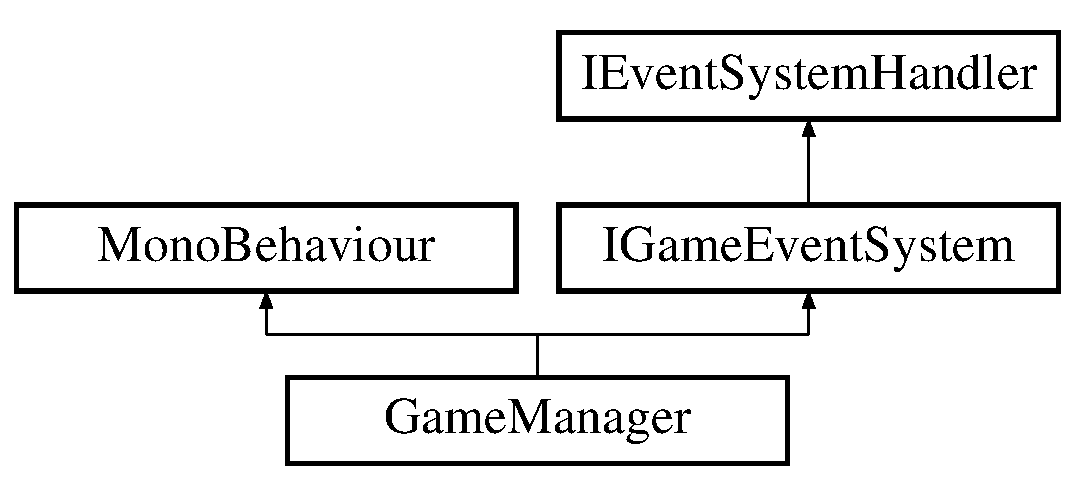
\includegraphics[height=3.000000cm]{class_game_manager}
\end{center}
\end{figure}
\subsection*{Public Member Functions}
\begin{DoxyCompactItemize}
\item 
void \mbox{\hyperlink{class_game_manager_ad5ae8ae2e2fe74743e89e70b47563639}{Level\+Over}} ()
\item 
void \mbox{\hyperlink{class_game_manager_a8d69157cb6b97eabeff2374d8e9adeaf}{Game\+Over}} ()
\end{DoxyCompactItemize}
\subsection*{Public Attributes}
\begin{DoxyCompactItemize}
\item 
\mbox{\Hypertarget{class_game_manager_a2195c4ae8d753a31d968d7c8347668de}\label{class_game_manager_a2195c4ae8d753a31d968d7c8347668de}} 
float {\bfseries level\+Start\+Delay} = 2f
\item 
\mbox{\Hypertarget{class_game_manager_a7b315d0972b05be3ed9c011ae09d5231}\label{class_game_manager_a7b315d0972b05be3ed9c011ae09d5231}} 
\mbox{\hyperlink{class_level_manager}{Level\+Manager}} {\bfseries level\+Manager}
\item 
\mbox{\Hypertarget{class_game_manager_a6b205783f48dd535e8db182d69e55ed7}\label{class_game_manager_a6b205783f48dd535e8db182d69e55ed7}} 
Game\+Object {\bfseries main\+Character}
\item 
\mbox{\Hypertarget{class_game_manager_a7840e876ed4c196856834b1d144033cc}\label{class_game_manager_a7840e876ed4c196856834b1d144033cc}} 
Game\+Object \mbox{[}$\,$\mbox{]} {\bfseries main\+Characters}
\end{DoxyCompactItemize}
\subsection*{Static Public Attributes}
\begin{DoxyCompactItemize}
\item 
\mbox{\Hypertarget{class_game_manager_a7666e8468dac197b9eb32dd32128524f}\label{class_game_manager_a7666e8468dac197b9eb32dd32128524f}} 
static \mbox{\hyperlink{class_game_manager}{Game\+Manager}} {\bfseries instance} = null
\end{DoxyCompactItemize}


\subsection{Member Function Documentation}
\mbox{\Hypertarget{class_game_manager_a8d69157cb6b97eabeff2374d8e9adeaf}\label{class_game_manager_a8d69157cb6b97eabeff2374d8e9adeaf}} 
\index{Game\+Manager@{Game\+Manager}!Game\+Over@{Game\+Over}}
\index{Game\+Over@{Game\+Over}!Game\+Manager@{Game\+Manager}}
\subsubsection{\texorpdfstring{Game\+Over()}{GameOver()}}
{\footnotesize\ttfamily void Game\+Manager.\+Game\+Over (\begin{DoxyParamCaption}{ }\end{DoxyParamCaption})\hspace{0.3cm}{\ttfamily [inline]}}


\begin{DoxyParams}{Parameters}
{\em none} & \\
\hline
\end{DoxyParams}
\begin{DoxyReturn}{Returns}
none Loads teh game over scene 
\end{DoxyReturn}


Implements \mbox{\hyperlink{interface_i_game_event_system_ab5c4b8b1d1a6fe358eb2ac3ffa93d835}{I\+Game\+Event\+System}}.

\mbox{\Hypertarget{class_game_manager_ad5ae8ae2e2fe74743e89e70b47563639}\label{class_game_manager_ad5ae8ae2e2fe74743e89e70b47563639}} 
\index{Game\+Manager@{Game\+Manager}!Level\+Over@{Level\+Over}}
\index{Level\+Over@{Level\+Over}!Game\+Manager@{Game\+Manager}}
\subsubsection{\texorpdfstring{Level\+Over()}{LevelOver()}}
{\footnotesize\ttfamily void Game\+Manager.\+Level\+Over (\begin{DoxyParamCaption}{ }\end{DoxyParamCaption})\hspace{0.3cm}{\ttfamily [inline]}}


\begin{DoxyParams}{Parameters}
{\em none} & \\
\hline
\end{DoxyParams}
\begin{DoxyReturn}{Returns}
none Increments level 
\end{DoxyReturn}


Implements \mbox{\hyperlink{interface_i_game_event_system_a1088da77edf39eb4cbfc32a5771f1092}{I\+Game\+Event\+System}}.



The documentation for this class was generated from the following file\+:\begin{DoxyCompactItemize}
\item 
Game\+Manager.\+cs\end{DoxyCompactItemize}

\hypertarget{class_game_music}{}\section{Game\+Music Class Reference}
\label{class_game_music}\index{Game\+Music@{Game\+Music}}
Inheritance diagram for Game\+Music\+:\begin{figure}[H]
\begin{center}
\leavevmode
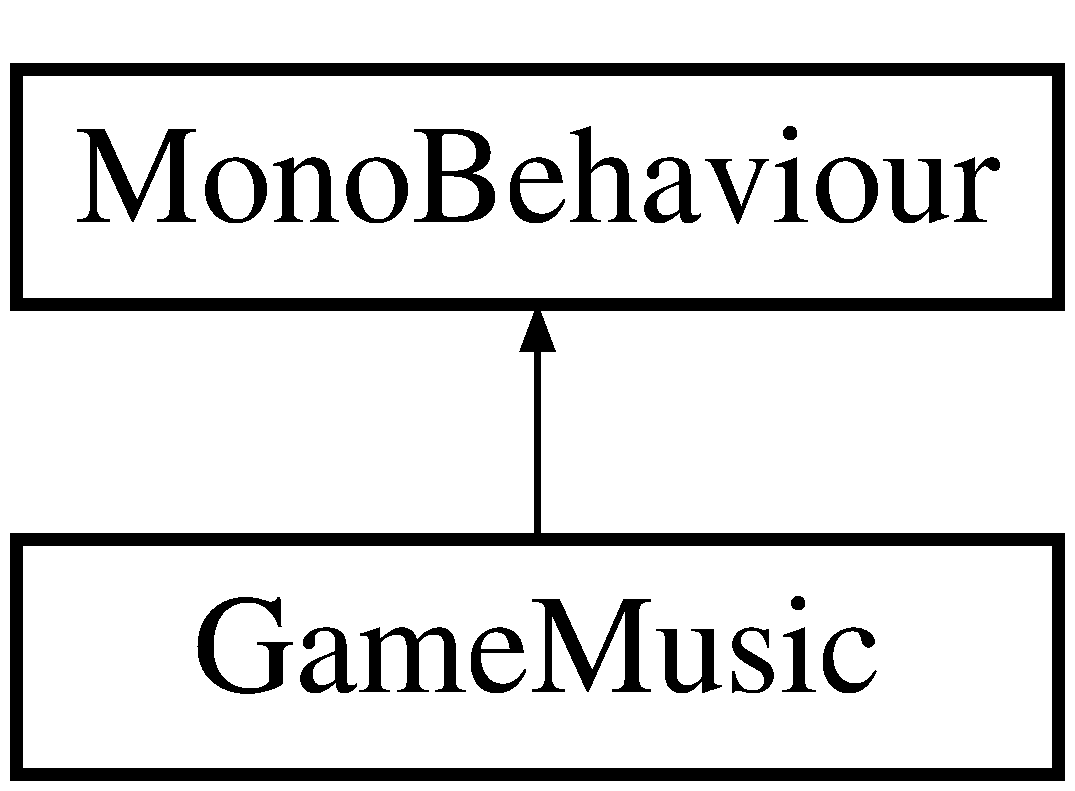
\includegraphics[height=2.000000cm]{class_game_music}
\end{center}
\end{figure}
\subsection*{Public Member Functions}
\begin{DoxyCompactItemize}
\item 
void \mbox{\hyperlink{class_game_music_ae88b1b78f9172cf9e69974c27819eee1}{Awake}} ()
\end{DoxyCompactItemize}


\subsection{Member Function Documentation}
\mbox{\Hypertarget{class_game_music_ae88b1b78f9172cf9e69974c27819eee1}\label{class_game_music_ae88b1b78f9172cf9e69974c27819eee1}} 
\index{Game\+Music@{Game\+Music}!Awake@{Awake}}
\index{Awake@{Awake}!Game\+Music@{Game\+Music}}
\subsubsection{\texorpdfstring{Awake()}{Awake()}}
{\footnotesize\ttfamily void Game\+Music.\+Awake (\begin{DoxyParamCaption}{ }\end{DoxyParamCaption})\hspace{0.3cm}{\ttfamily [inline]}}

Awake 
\begin{DoxyParams}{Parameters}
{\em none} & \\
\hline
\end{DoxyParams}
\begin{DoxyReturn}{Returns}
none Stops the menu music and starts the game music Also only allows one instance of game music to play 
\end{DoxyReturn}


The documentation for this class was generated from the following file\+:\begin{DoxyCompactItemize}
\item 
Game\+Music.\+cs\end{DoxyCompactItemize}

\hypertarget{class_game_over}{}\section{Game\+Over Class Reference}
\label{class_game_over}\index{Game\+Over@{Game\+Over}}
Inheritance diagram for Game\+Over\+:\begin{figure}[H]
\begin{center}
\leavevmode
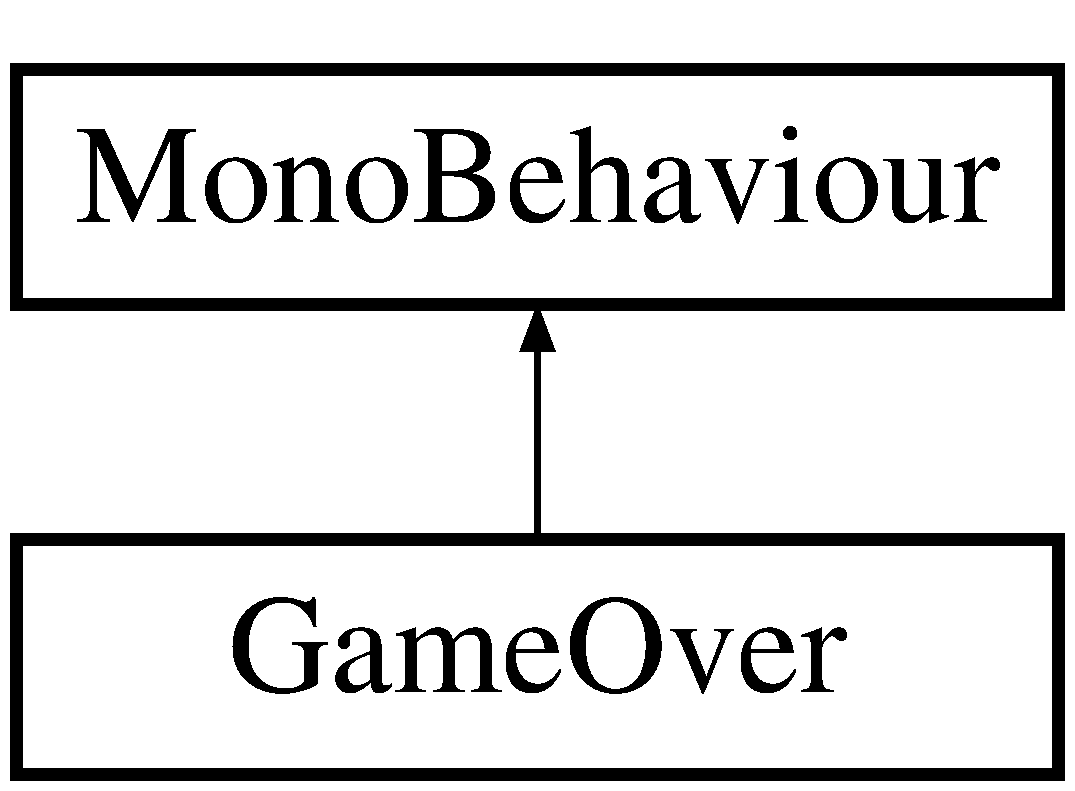
\includegraphics[height=2.000000cm]{class_game_over}
\end{center}
\end{figure}
\subsection*{Public Member Functions}
\begin{DoxyCompactItemize}
\item 
void \mbox{\hyperlink{class_game_over_a9fef6c386d51e0cea3c9d4f941c66289}{Awake}} ()
\item 
void \mbox{\hyperlink{class_game_over_a01c0b3e1f8612df9ebd5675ba0719beb}{Show\+Leaderboard}} ()
\item 
void \mbox{\hyperlink{class_game_over_af7a0b3719580737182a952c8fb487232}{to\+Main\+Menu}} ()
\item 
void \mbox{\hyperlink{class_game_over_a252e97e89fa007889c2a9fb4a2f9b06c}{Quit\+Game}} ()
\end{DoxyCompactItemize}


\subsection{Member Function Documentation}
\mbox{\Hypertarget{class_game_over_a9fef6c386d51e0cea3c9d4f941c66289}\label{class_game_over_a9fef6c386d51e0cea3c9d4f941c66289}} 
\index{Game\+Over@{Game\+Over}!Awake@{Awake}}
\index{Awake@{Awake}!Game\+Over@{Game\+Over}}
\subsubsection{\texorpdfstring{Awake()}{Awake()}}
{\footnotesize\ttfamily void Game\+Over.\+Awake (\begin{DoxyParamCaption}{ }\end{DoxyParamCaption})\hspace{0.3cm}{\ttfamily [inline]}}

Awake 
\begin{DoxyParams}{Parameters}
{\em none} & \\
\hline
\end{DoxyParams}
\begin{DoxyReturn}{Returns}
none Starts the Game Over scene 
\end{DoxyReturn}
\mbox{\Hypertarget{class_game_over_a252e97e89fa007889c2a9fb4a2f9b06c}\label{class_game_over_a252e97e89fa007889c2a9fb4a2f9b06c}} 
\index{Game\+Over@{Game\+Over}!Quit\+Game@{Quit\+Game}}
\index{Quit\+Game@{Quit\+Game}!Game\+Over@{Game\+Over}}
\subsubsection{\texorpdfstring{Quit\+Game()}{QuitGame()}}
{\footnotesize\ttfamily void Game\+Over.\+Quit\+Game (\begin{DoxyParamCaption}{ }\end{DoxyParamCaption})\hspace{0.3cm}{\ttfamily [inline]}}

Quit\+Game 
\begin{DoxyParams}{Parameters}
{\em none} & \\
\hline
\end{DoxyParams}
\begin{DoxyReturn}{Returns}
none exits the game 
\end{DoxyReturn}
\mbox{\Hypertarget{class_game_over_a01c0b3e1f8612df9ebd5675ba0719beb}\label{class_game_over_a01c0b3e1f8612df9ebd5675ba0719beb}} 
\index{Game\+Over@{Game\+Over}!Show\+Leaderboard@{Show\+Leaderboard}}
\index{Show\+Leaderboard@{Show\+Leaderboard}!Game\+Over@{Game\+Over}}
\subsubsection{\texorpdfstring{Show\+Leaderboard()}{ShowLeaderboard()}}
{\footnotesize\ttfamily void Game\+Over.\+Show\+Leaderboard (\begin{DoxyParamCaption}{ }\end{DoxyParamCaption})\hspace{0.3cm}{\ttfamily [inline]}}

Show\+Leaderboard 
\begin{DoxyParams}{Parameters}
{\em none} & \\
\hline
\end{DoxyParams}
\begin{DoxyReturn}{Returns}
none shows the leaderboard 
\end{DoxyReturn}
\mbox{\Hypertarget{class_game_over_af7a0b3719580737182a952c8fb487232}\label{class_game_over_af7a0b3719580737182a952c8fb487232}} 
\index{Game\+Over@{Game\+Over}!to\+Main\+Menu@{to\+Main\+Menu}}
\index{to\+Main\+Menu@{to\+Main\+Menu}!Game\+Over@{Game\+Over}}
\subsubsection{\texorpdfstring{to\+Main\+Menu()}{toMainMenu()}}
{\footnotesize\ttfamily void Game\+Over.\+to\+Main\+Menu (\begin{DoxyParamCaption}{ }\end{DoxyParamCaption})\hspace{0.3cm}{\ttfamily [inline]}}

Loads \mbox{\hyperlink{class_main_menu}{Main\+Menu}}  None  None 

The documentation for this class was generated from the following file\+:\begin{DoxyCompactItemize}
\item 
Game\+Over.\+cs\end{DoxyCompactItemize}

\hypertarget{class_gingy}{}\section{Gingy Class Reference}
\label{class_gingy}\index{Gingy@{Gingy}}
Inheritance diagram for Gingy\+:\begin{figure}[H]
\begin{center}
\leavevmode
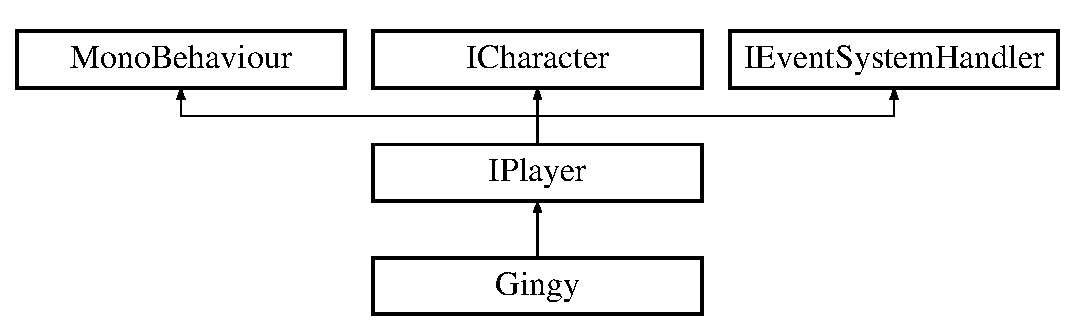
\includegraphics[height=3.000000cm]{class_gingy}
\end{center}
\end{figure}
\subsection*{Public Member Functions}
\begin{DoxyCompactItemize}
\item 
int \mbox{\hyperlink{class_gingy_ae36218bf9d6ae39c9176da509d67f007}{Get\+Health}} ()
\item 
void \mbox{\hyperlink{class_gingy_a47954df8d4b796088a54e147be4b789d}{Set\+Health}} (int value)
\end{DoxyCompactItemize}
\subsection*{Additional Inherited Members}


\subsection{Member Function Documentation}
\mbox{\Hypertarget{class_gingy_ae36218bf9d6ae39c9176da509d67f007}\label{class_gingy_ae36218bf9d6ae39c9176da509d67f007}} 
\index{Gingy@{Gingy}!Get\+Health@{Get\+Health}}
\index{Get\+Health@{Get\+Health}!Gingy@{Gingy}}
\subsubsection{\texorpdfstring{Get\+Health()}{GetHealth()}}
{\footnotesize\ttfamily int Gingy.\+Get\+Health (\begin{DoxyParamCaption}{ }\end{DoxyParamCaption})\hspace{0.3cm}{\ttfamily [inline]}}

Get\+Health 
\begin{DoxyParams}{Parameters}
{\em none} & \\
\hline
\end{DoxyParams}
\begin{DoxyReturn}{Returns}
int returns health 
\end{DoxyReturn}
\mbox{\Hypertarget{class_gingy_a47954df8d4b796088a54e147be4b789d}\label{class_gingy_a47954df8d4b796088a54e147be4b789d}} 
\index{Gingy@{Gingy}!Set\+Health@{Set\+Health}}
\index{Set\+Health@{Set\+Health}!Gingy@{Gingy}}
\subsubsection{\texorpdfstring{Set\+Health()}{SetHealth()}}
{\footnotesize\ttfamily void Gingy.\+Set\+Health (\begin{DoxyParamCaption}\item[{int}]{value }\end{DoxyParamCaption})\hspace{0.3cm}{\ttfamily [inline]}}

Set\+Health 
\begin{DoxyParams}{Parameters}
{\em int} & \\
\hline
\end{DoxyParams}
\begin{DoxyReturn}{Returns}
none Sets the health 
\end{DoxyReturn}


The documentation for this class was generated from the following file\+:\begin{DoxyCompactItemize}
\item 
Gingy.\+cs\end{DoxyCompactItemize}

\hypertarget{class_health_bar_script}{}\section{Health\+Bar\+Script Class Reference}
\label{class_health_bar_script}\index{Health\+Bar\+Script@{Health\+Bar\+Script}}
Inheritance diagram for Health\+Bar\+Script\+:\begin{figure}[H]
\begin{center}
\leavevmode
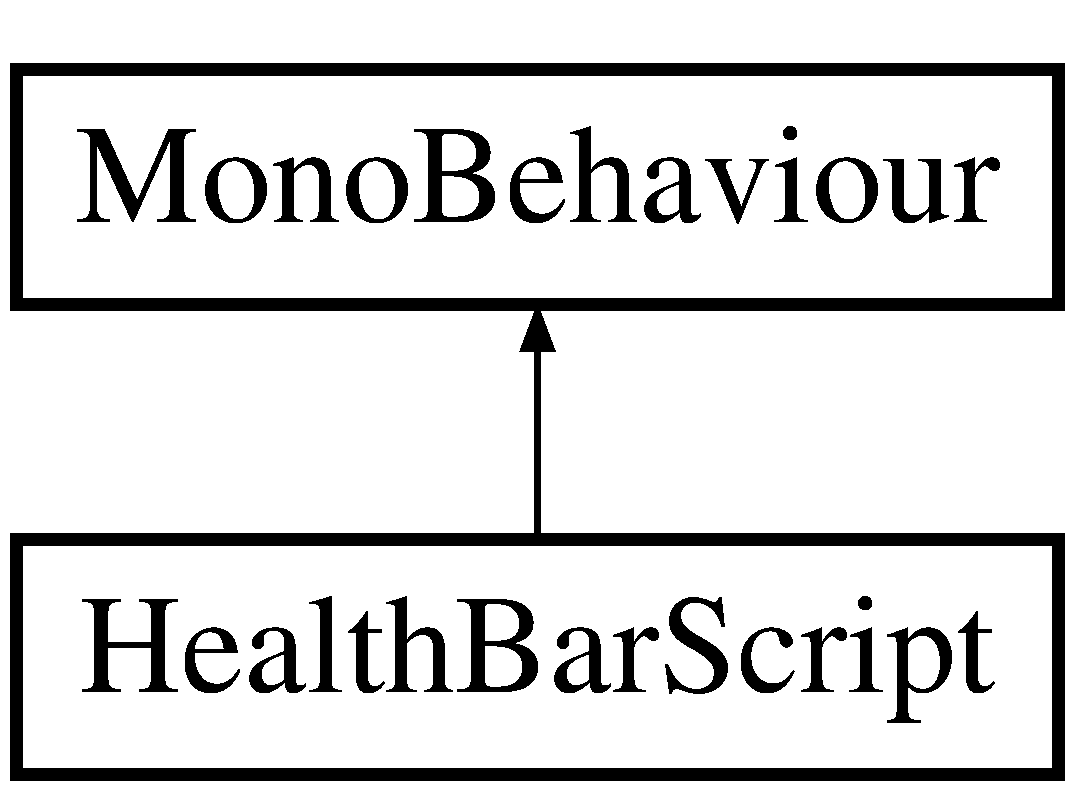
\includegraphics[height=2.000000cm]{class_health_bar_script}
\end{center}
\end{figure}
\subsection*{Static Public Attributes}
\begin{DoxyCompactItemize}
\item 
\mbox{\Hypertarget{class_health_bar_script_a3ee24ea7a76f5141550424cdb9021df5}\label{class_health_bar_script_a3ee24ea7a76f5141550424cdb9021df5}} 
static float {\bfseries health}
\end{DoxyCompactItemize}


The documentation for this class was generated from the following file\+:\begin{DoxyCompactItemize}
\item 
Health\+Bar\+Script.\+cs\end{DoxyCompactItemize}

\hypertarget{classhealth_item}{}\section{health\+Item Class Reference}
\label{classhealth_item}\index{health\+Item@{health\+Item}}
Inheritance diagram for health\+Item\+:\begin{figure}[H]
\begin{center}
\leavevmode
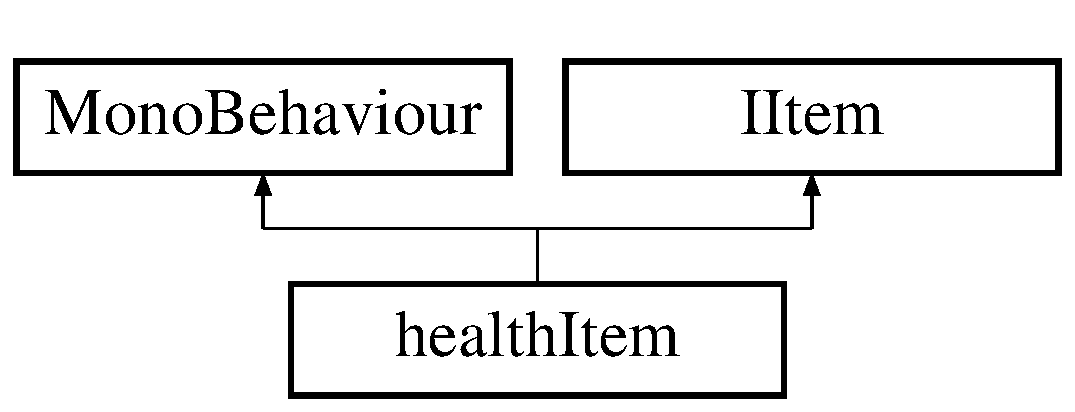
\includegraphics[height=2.000000cm]{classhealth_item}
\end{center}
\end{figure}
\subsection*{Public Member Functions}
\begin{DoxyCompactItemize}
\item 
void \mbox{\hyperlink{classhealth_item_a86f0e7f02919e7daa4076717a3a0acac}{Ability}} (\mbox{\hyperlink{class_i_player}{I\+Player}} player)
\item 
void \mbox{\hyperlink{classhealth_item_a545574879140f4c98b388f1dc7d2a7f8}{Duration}} (\mbox{\hyperlink{class_i_player}{I\+Player}} player)
\end{DoxyCompactItemize}


\subsection{Member Function Documentation}
\mbox{\Hypertarget{classhealth_item_a86f0e7f02919e7daa4076717a3a0acac}\label{classhealth_item_a86f0e7f02919e7daa4076717a3a0acac}} 
\index{health\+Item@{health\+Item}!Ability@{Ability}}
\index{Ability@{Ability}!health\+Item@{health\+Item}}
\subsubsection{\texorpdfstring{Ability()}{Ability()}}
{\footnotesize\ttfamily void health\+Item.\+Ability (\begin{DoxyParamCaption}\item[{\mbox{\hyperlink{class_i_player}{I\+Player}}}]{player }\end{DoxyParamCaption})\hspace{0.3cm}{\ttfamily [inline]}}


\begin{DoxyParams}{Parameters}
{\em \mbox{\hyperlink{class_i_player}{I\+Player}}} & \\
\hline
\end{DoxyParams}
\begin{DoxyReturn}{Returns}
none Calls the ability of the item 
\end{DoxyReturn}


Implements \mbox{\hyperlink{interface_i_item_afe73efbf8316273df20162d6f4b20648}{I\+Item}}.

\mbox{\Hypertarget{classhealth_item_a545574879140f4c98b388f1dc7d2a7f8}\label{classhealth_item_a545574879140f4c98b388f1dc7d2a7f8}} 
\index{health\+Item@{health\+Item}!Duration@{Duration}}
\index{Duration@{Duration}!health\+Item@{health\+Item}}
\subsubsection{\texorpdfstring{Duration()}{Duration()}}
{\footnotesize\ttfamily void health\+Item.\+Duration (\begin{DoxyParamCaption}\item[{\mbox{\hyperlink{class_i_player}{I\+Player}}}]{player }\end{DoxyParamCaption})\hspace{0.3cm}{\ttfamily [inline]}}


\begin{DoxyParams}{Parameters}
{\em \mbox{\hyperlink{class_i_player}{I\+Player}}} & \\
\hline
\end{DoxyParams}
\begin{DoxyReturn}{Returns}
none does nothing 
\end{DoxyReturn}


Implements \mbox{\hyperlink{interface_i_item_a797c1d62a7828bf428cc486ceaf18e9c}{I\+Item}}.



The documentation for this class was generated from the following file\+:\begin{DoxyCompactItemize}
\item 
health\+Item.\+cs\end{DoxyCompactItemize}

\hypertarget{class_health_item_spawner}{}\section{Health\+Item\+Spawner Class Reference}
\label{class_health_item_spawner}\index{Health\+Item\+Spawner@{Health\+Item\+Spawner}}
Inheritance diagram for Health\+Item\+Spawner\+:\begin{figure}[H]
\begin{center}
\leavevmode
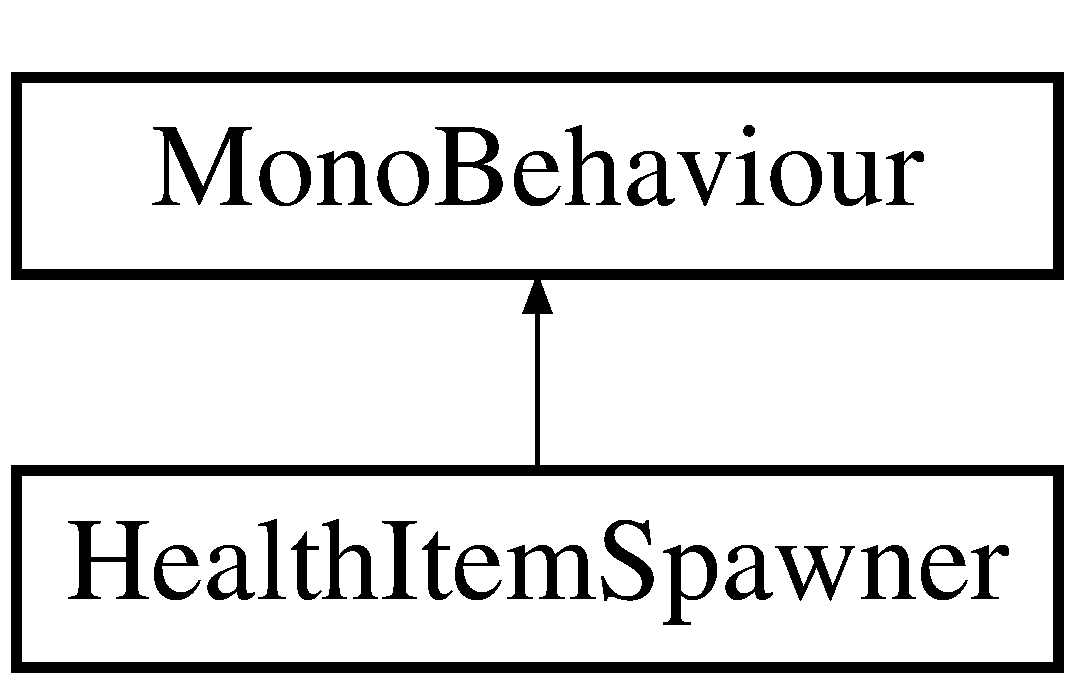
\includegraphics[height=2.000000cm]{class_health_item_spawner}
\end{center}
\end{figure}
\subsection*{Public Attributes}
\begin{DoxyCompactItemize}
\item 
\mbox{\Hypertarget{class_health_item_spawner_a4d41421ba0d81611bbeba19904cf6a96}\label{class_health_item_spawner_a4d41421ba0d81611bbeba19904cf6a96}} 
Game\+Object {\bfseries health\+Item}
\end{DoxyCompactItemize}


The documentation for this class was generated from the following file\+:\begin{DoxyCompactItemize}
\item 
Health\+Item\+Spawner.\+cs\end{DoxyCompactItemize}

\hypertarget{interface_i_character}{}\section{I\+Character Interface Reference}
\label{interface_i_character}\index{I\+Character@{I\+Character}}
Inheritance diagram for I\+Character\+:\begin{figure}[H]
\begin{center}
\leavevmode
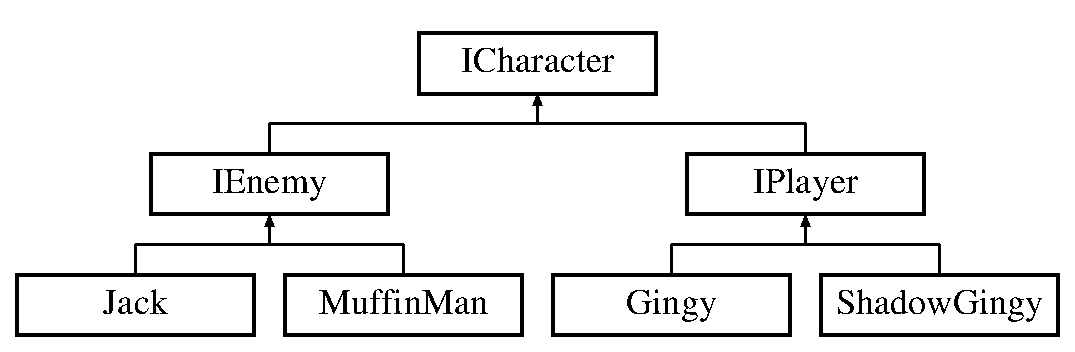
\includegraphics[height=3.000000cm]{interface_i_character}
\end{center}
\end{figure}
\subsection*{Public Member Functions}
\begin{DoxyCompactItemize}
\item 
\mbox{\Hypertarget{interface_i_character_a5ff82ed63ab6c5f142ee2222f1e7164b}\label{interface_i_character_a5ff82ed63ab6c5f142ee2222f1e7164b}} 
void {\bfseries Take\+Damage} (int damage\+Taken)
\item 
\mbox{\Hypertarget{interface_i_character_adeba1d21cd6df9251ae45eea19d47672}\label{interface_i_character_adeba1d21cd6df9251ae45eea19d47672}} 
void {\bfseries Attack} ()
\item 
\mbox{\Hypertarget{interface_i_character_a3e5e2be6e9b94d6305c4f04ec7250af4}\label{interface_i_character_a3e5e2be6e9b94d6305c4f04ec7250af4}} 
void {\bfseries set\+Speed} (int speed)
\item 
\mbox{\Hypertarget{interface_i_character_a8ba692ee17ea30254bebbafd74f0bea4}\label{interface_i_character_a8ba692ee17ea30254bebbafd74f0bea4}} 
void {\bfseries set\+Health} (int health)
\item 
\mbox{\Hypertarget{interface_i_character_a62ddd177f869258efdcf171dd8284009}\label{interface_i_character_a62ddd177f869258efdcf171dd8284009}} 
bool {\bfseries is\+Dead} ()
\item 
void \mbox{\hyperlink{interface_i_character_ad58356e457f98d8a6f9548da446012ce}{Die}} ()
\end{DoxyCompactItemize}


\subsection{Member Function Documentation}
\mbox{\Hypertarget{interface_i_character_ad58356e457f98d8a6f9548da446012ce}\label{interface_i_character_ad58356e457f98d8a6f9548da446012ce}} 
\index{I\+Character@{I\+Character}!Die@{Die}}
\index{Die@{Die}!I\+Character@{I\+Character}}
\subsubsection{\texorpdfstring{Die()}{Die()}}
{\footnotesize\ttfamily void I\+Character.\+Die (\begin{DoxyParamCaption}{ }\end{DoxyParamCaption})}

Destroys the characted when it dies  None  None 

Implemented in \mbox{\hyperlink{class_i_player_a62499ee0288916e1220f64e18653c7b7}{I\+Player}}, and \mbox{\hyperlink{class_i_enemy_a53c76db616e0e102f1ddd3cfe2c8ed28}{I\+Enemy}}.



The documentation for this interface was generated from the following file\+:\begin{DoxyCompactItemize}
\item 
I\+Character.\+cs\end{DoxyCompactItemize}

\hypertarget{class_i_enemy}{}\section{I\+Enemy Class Reference}
\label{class_i_enemy}\index{I\+Enemy@{I\+Enemy}}
Inheritance diagram for I\+Enemy\+:\begin{figure}[H]
\begin{center}
\leavevmode
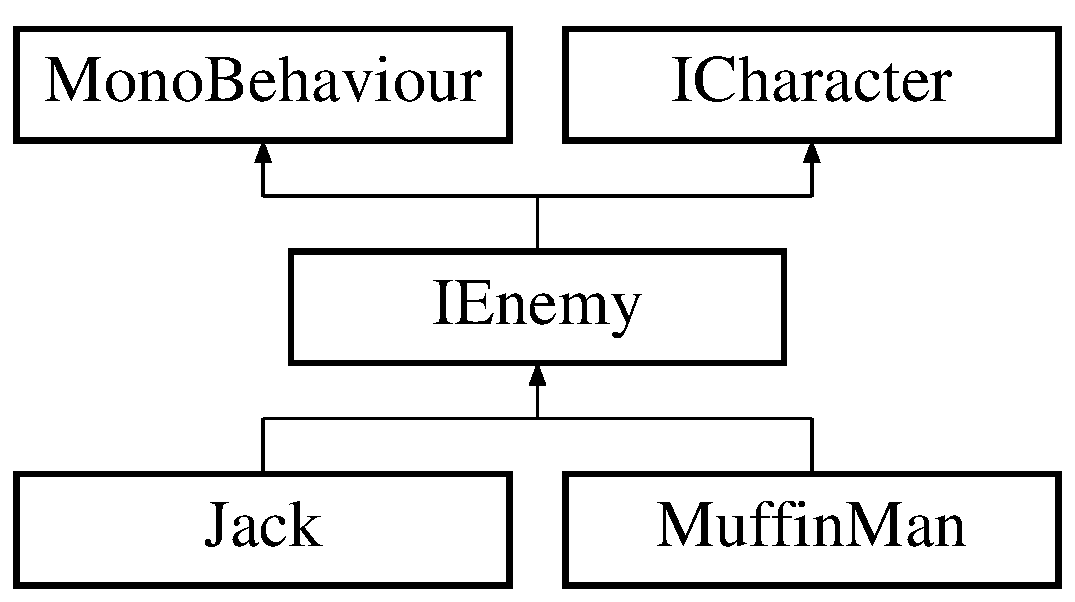
\includegraphics[height=3.000000cm]{class_i_enemy}
\end{center}
\end{figure}
\subsection*{Public Member Functions}
\begin{DoxyCompactItemize}
\item 
void \mbox{\hyperlink{class_i_enemy_af9c3000cf4db4888aa1be7e6db70240f}{Take\+Damage}} (int damage\+Taken)
\item 
void \mbox{\hyperlink{class_i_enemy_aa7214edc7d35f1684009bba6f34387b7}{Attack}} ()
\item 
void \mbox{\hyperlink{class_i_enemy_aef93bc3d389f8b290b0eb4f12dc329f4}{set\+Speed}} (int speed)
\item 
void \mbox{\hyperlink{class_i_enemy_aa8f554e318bad0827c6186e6ae46fbd4}{set\+Health}} (int health)
\item 
bool \mbox{\hyperlink{class_i_enemy_ab4b9b90ff23a48388ba9fb3fd794a282}{is\+Dead}} ()
\item 
void \mbox{\hyperlink{class_i_enemy_a53c76db616e0e102f1ddd3cfe2c8ed28}{Die}} ()
\end{DoxyCompactItemize}
\subsection*{Public Attributes}
\begin{DoxyCompactItemize}
\item 
\mbox{\Hypertarget{class_i_enemy_a6310c4cf55e1e5814fd9f1c19c9acc2d}\label{class_i_enemy_a6310c4cf55e1e5814fd9f1c19c9acc2d}} 
int {\bfseries Health} = 100
\item 
\mbox{\Hypertarget{class_i_enemy_a03e4a34e8acaba49dd074feeb12e1e55}\label{class_i_enemy_a03e4a34e8acaba49dd074feeb12e1e55}} 
string {\bfseries enemy\+Name}
\end{DoxyCompactItemize}


\subsection{Member Function Documentation}
\mbox{\Hypertarget{class_i_enemy_aa7214edc7d35f1684009bba6f34387b7}\label{class_i_enemy_aa7214edc7d35f1684009bba6f34387b7}} 
\index{I\+Enemy@{I\+Enemy}!Attack@{Attack}}
\index{Attack@{Attack}!I\+Enemy@{I\+Enemy}}
\subsubsection{\texorpdfstring{Attack()}{Attack()}}
{\footnotesize\ttfamily void I\+Enemy.\+Attack (\begin{DoxyParamCaption}{ }\end{DoxyParamCaption})\hspace{0.3cm}{\ttfamily [inline]}}

Void  None  None 

Implements \mbox{\hyperlink{interface_i_character}{I\+Character}}.

\mbox{\Hypertarget{class_i_enemy_a53c76db616e0e102f1ddd3cfe2c8ed28}\label{class_i_enemy_a53c76db616e0e102f1ddd3cfe2c8ed28}} 
\index{I\+Enemy@{I\+Enemy}!Die@{Die}}
\index{Die@{Die}!I\+Enemy@{I\+Enemy}}
\subsubsection{\texorpdfstring{Die()}{Die()}}
{\footnotesize\ttfamily void I\+Enemy.\+Die (\begin{DoxyParamCaption}{ }\end{DoxyParamCaption})\hspace{0.3cm}{\ttfamily [inline]}}

Destroys the character when it dies  None  None 

Implements \mbox{\hyperlink{interface_i_character_ad58356e457f98d8a6f9548da446012ce}{I\+Character}}.

\mbox{\Hypertarget{class_i_enemy_ab4b9b90ff23a48388ba9fb3fd794a282}\label{class_i_enemy_ab4b9b90ff23a48388ba9fb3fd794a282}} 
\index{I\+Enemy@{I\+Enemy}!is\+Dead@{is\+Dead}}
\index{is\+Dead@{is\+Dead}!I\+Enemy@{I\+Enemy}}
\subsubsection{\texorpdfstring{is\+Dead()}{isDead()}}
{\footnotesize\ttfamily bool I\+Enemy.\+is\+Dead (\begin{DoxyParamCaption}{ }\end{DoxyParamCaption})\hspace{0.3cm}{\ttfamily [inline]}}

Returns True if the player is dead and returns false if the player is not dead  None  Bool 

Implements \mbox{\hyperlink{interface_i_character}{I\+Character}}.

\mbox{\Hypertarget{class_i_enemy_aa8f554e318bad0827c6186e6ae46fbd4}\label{class_i_enemy_aa8f554e318bad0827c6186e6ae46fbd4}} 
\index{I\+Enemy@{I\+Enemy}!set\+Health@{set\+Health}}
\index{set\+Health@{set\+Health}!I\+Enemy@{I\+Enemy}}
\subsubsection{\texorpdfstring{set\+Health()}{setHealth()}}
{\footnotesize\ttfamily void I\+Enemy.\+set\+Health (\begin{DoxyParamCaption}\item[{int}]{health }\end{DoxyParamCaption})\hspace{0.3cm}{\ttfamily [inline]}}

Void  int Health  None 

Implements \mbox{\hyperlink{interface_i_character}{I\+Character}}.

\mbox{\Hypertarget{class_i_enemy_aef93bc3d389f8b290b0eb4f12dc329f4}\label{class_i_enemy_aef93bc3d389f8b290b0eb4f12dc329f4}} 
\index{I\+Enemy@{I\+Enemy}!set\+Speed@{set\+Speed}}
\index{set\+Speed@{set\+Speed}!I\+Enemy@{I\+Enemy}}
\subsubsection{\texorpdfstring{set\+Speed()}{setSpeed()}}
{\footnotesize\ttfamily void I\+Enemy.\+set\+Speed (\begin{DoxyParamCaption}\item[{int}]{speed }\end{DoxyParamCaption})\hspace{0.3cm}{\ttfamily [inline]}}

Void  int Speed  None 

Implements \mbox{\hyperlink{interface_i_character}{I\+Character}}.

\mbox{\Hypertarget{class_i_enemy_af9c3000cf4db4888aa1be7e6db70240f}\label{class_i_enemy_af9c3000cf4db4888aa1be7e6db70240f}} 
\index{I\+Enemy@{I\+Enemy}!Take\+Damage@{Take\+Damage}}
\index{Take\+Damage@{Take\+Damage}!I\+Enemy@{I\+Enemy}}
\subsubsection{\texorpdfstring{Take\+Damage()}{TakeDamage()}}
{\footnotesize\ttfamily void I\+Enemy.\+Take\+Damage (\begin{DoxyParamCaption}\item[{int}]{damage\+Taken }\end{DoxyParamCaption})\hspace{0.3cm}{\ttfamily [inline]}}

Does Damage to a player when it is struck by an enemy  Damage Taken  bool 

Implements \mbox{\hyperlink{interface_i_character}{I\+Character}}.



The documentation for this class was generated from the following file\+:\begin{DoxyCompactItemize}
\item 
I\+Enemy.\+cs\end{DoxyCompactItemize}

\hypertarget{interface_i_game_event_system}{}\section{I\+Game\+Event\+System Interface Reference}
\label{interface_i_game_event_system}\index{I\+Game\+Event\+System@{I\+Game\+Event\+System}}
Inheritance diagram for I\+Game\+Event\+System\+:\begin{figure}[H]
\begin{center}
\leavevmode
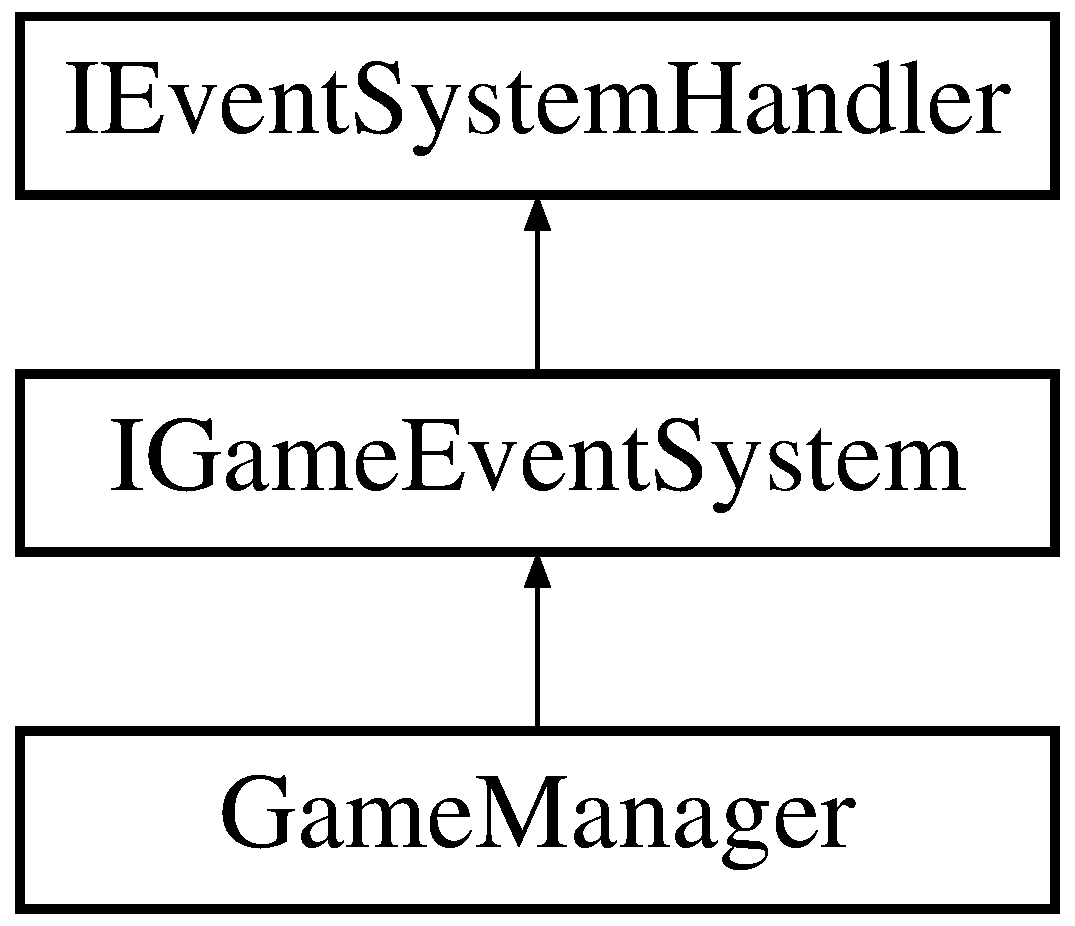
\includegraphics[height=3.000000cm]{interface_i_game_event_system}
\end{center}
\end{figure}
\subsection*{Public Member Functions}
\begin{DoxyCompactItemize}
\item 
void \mbox{\hyperlink{interface_i_game_event_system_a1088da77edf39eb4cbfc32a5771f1092}{Level\+Over}} ()
\item 
void \mbox{\hyperlink{interface_i_game_event_system_ab5c4b8b1d1a6fe358eb2ac3ffa93d835}{Game\+Over}} ()
\end{DoxyCompactItemize}


\subsection{Member Function Documentation}
\mbox{\Hypertarget{interface_i_game_event_system_ab5c4b8b1d1a6fe358eb2ac3ffa93d835}\label{interface_i_game_event_system_ab5c4b8b1d1a6fe358eb2ac3ffa93d835}} 
\index{I\+Game\+Event\+System@{I\+Game\+Event\+System}!Game\+Over@{Game\+Over}}
\index{Game\+Over@{Game\+Over}!I\+Game\+Event\+System@{I\+Game\+Event\+System}}
\subsubsection{\texorpdfstring{Game\+Over()}{GameOver()}}
{\footnotesize\ttfamily void I\+Game\+Event\+System.\+Game\+Over (\begin{DoxyParamCaption}{ }\end{DoxyParamCaption})}


\begin{DoxyParams}{Parameters}
{\em none} & \\
\hline
\end{DoxyParams}
\begin{DoxyReturn}{Returns}
none Use of the eventsystemhandler to message game over 
\end{DoxyReturn}


Implemented in \mbox{\hyperlink{class_game_manager_a8d69157cb6b97eabeff2374d8e9adeaf}{Game\+Manager}}.

\mbox{\Hypertarget{interface_i_game_event_system_a1088da77edf39eb4cbfc32a5771f1092}\label{interface_i_game_event_system_a1088da77edf39eb4cbfc32a5771f1092}} 
\index{I\+Game\+Event\+System@{I\+Game\+Event\+System}!Level\+Over@{Level\+Over}}
\index{Level\+Over@{Level\+Over}!I\+Game\+Event\+System@{I\+Game\+Event\+System}}
\subsubsection{\texorpdfstring{Level\+Over()}{LevelOver()}}
{\footnotesize\ttfamily void I\+Game\+Event\+System.\+Level\+Over (\begin{DoxyParamCaption}{ }\end{DoxyParamCaption})}


\begin{DoxyParams}{Parameters}
{\em none} & \\
\hline
\end{DoxyParams}
\begin{DoxyReturn}{Returns}
none Use of the eventsystemhandler to message level over 
\end{DoxyReturn}


Implemented in \mbox{\hyperlink{class_game_manager_ad5ae8ae2e2fe74743e89e70b47563639}{Game\+Manager}}.



The documentation for this interface was generated from the following file\+:\begin{DoxyCompactItemize}
\item 
I\+Game\+Event\+System.\+cs\end{DoxyCompactItemize}

\hypertarget{interface_i_item}{}\section{I\+Item Interface Reference}
\label{interface_i_item}\index{I\+Item@{I\+Item}}
Inheritance diagram for I\+Item\+:\begin{figure}[H]
\begin{center}
\leavevmode
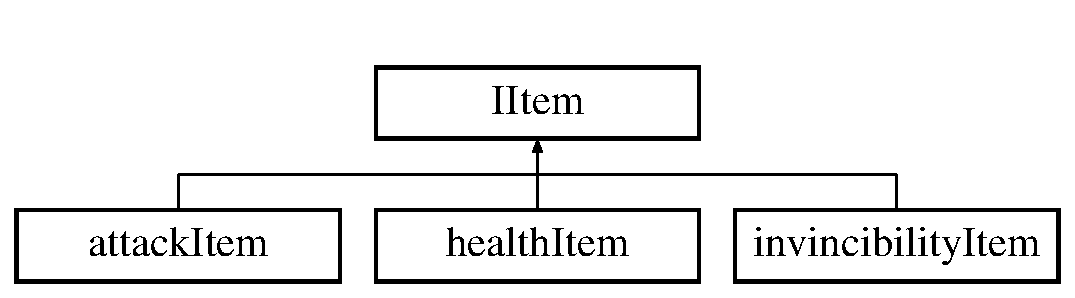
\includegraphics[height=2.000000cm]{interface_i_item}
\end{center}
\end{figure}
\subsection*{Public Member Functions}
\begin{DoxyCompactItemize}
\item 
void \mbox{\hyperlink{interface_i_item_afe73efbf8316273df20162d6f4b20648}{Ability}} (\mbox{\hyperlink{class_i_player}{I\+Player}} player)
\item 
void \mbox{\hyperlink{interface_i_item_a797c1d62a7828bf428cc486ceaf18e9c}{Duration}} (\mbox{\hyperlink{class_i_player}{I\+Player}} player)
\end{DoxyCompactItemize}


\subsection{Member Function Documentation}
\mbox{\Hypertarget{interface_i_item_afe73efbf8316273df20162d6f4b20648}\label{interface_i_item_afe73efbf8316273df20162d6f4b20648}} 
\index{I\+Item@{I\+Item}!Ability@{Ability}}
\index{Ability@{Ability}!I\+Item@{I\+Item}}
\subsubsection{\texorpdfstring{Ability()}{Ability()}}
{\footnotesize\ttfamily void I\+Item.\+Ability (\begin{DoxyParamCaption}\item[{\mbox{\hyperlink{class_i_player}{I\+Player}}}]{player }\end{DoxyParamCaption})}

Determines the ability that the player recieves  player  None 

Implemented in \mbox{\hyperlink{classattack_item_ab5739e198a4a255f81d371df77bb770b}{attack\+Item}}, \mbox{\hyperlink{classhealth_item_a86f0e7f02919e7daa4076717a3a0acac}{health\+Item}}, and \mbox{\hyperlink{classinvincibility_item_a6fe1d452c0e956c50b4cb468b4bd140b}{invincibility\+Item}}.

\mbox{\Hypertarget{interface_i_item_a797c1d62a7828bf428cc486ceaf18e9c}\label{interface_i_item_a797c1d62a7828bf428cc486ceaf18e9c}} 
\index{I\+Item@{I\+Item}!Duration@{Duration}}
\index{Duration@{Duration}!I\+Item@{I\+Item}}
\subsubsection{\texorpdfstring{Duration()}{Duration()}}
{\footnotesize\ttfamily void I\+Item.\+Duration (\begin{DoxyParamCaption}\item[{\mbox{\hyperlink{class_i_player}{I\+Player}}}]{player }\end{DoxyParamCaption})}

Determines the duration of the ability  player  None 

Implemented in \mbox{\hyperlink{classattack_item_a5cf5ac415471d294a3244988466d54ac}{attack\+Item}}, \mbox{\hyperlink{classhealth_item_a545574879140f4c98b388f1dc7d2a7f8}{health\+Item}}, and \mbox{\hyperlink{classinvincibility_item_abe2368f3358065d15547f24e8cee2de5}{invincibility\+Item}}.



The documentation for this interface was generated from the following file\+:\begin{DoxyCompactItemize}
\item 
I\+Item.\+cs\end{DoxyCompactItemize}

\hypertarget{class_input_name}{}\section{Input\+Name Class Reference}
\label{class_input_name}\index{Input\+Name@{Input\+Name}}
Inheritance diagram for Input\+Name\+:\begin{figure}[H]
\begin{center}
\leavevmode
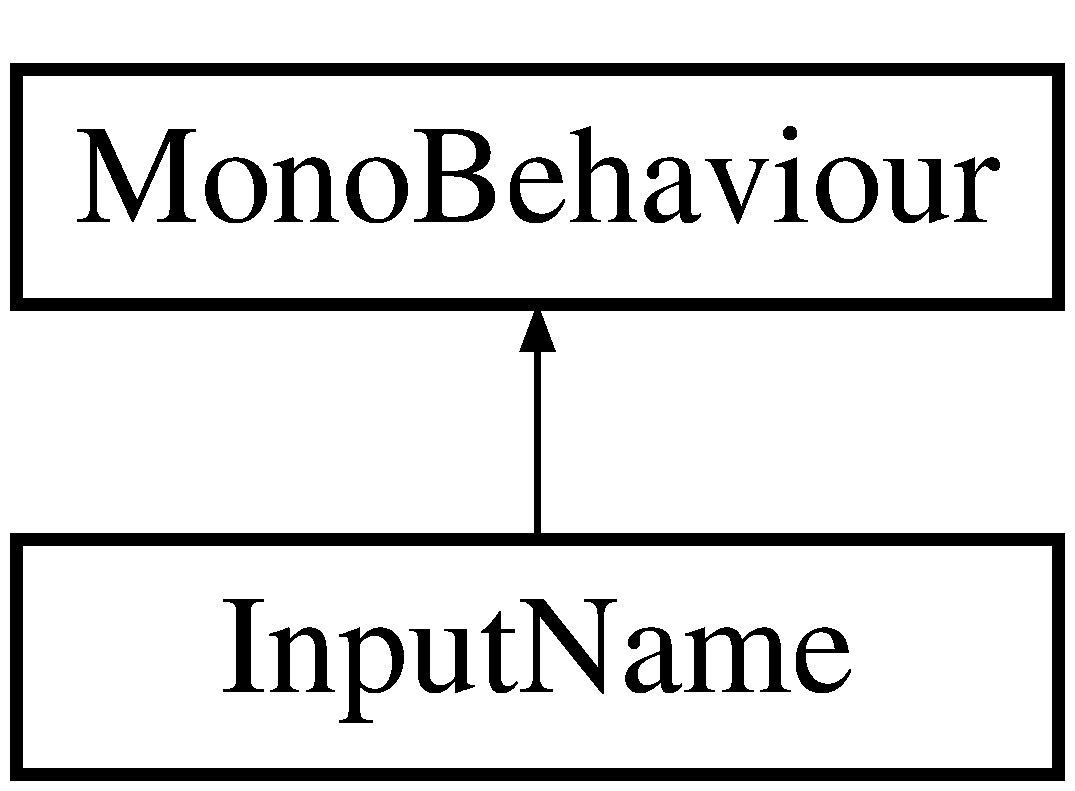
\includegraphics[height=2.000000cm]{class_input_name}
\end{center}
\end{figure}
\subsection*{Public Member Functions}
\begin{DoxyCompactItemize}
\item 
void \mbox{\hyperlink{class_input_name_af7ccce069e27f5fb0aea884e9d882d42}{Submit\+Name}} ()
\end{DoxyCompactItemize}


\subsection{Member Function Documentation}
\mbox{\Hypertarget{class_input_name_af7ccce069e27f5fb0aea884e9d882d42}\label{class_input_name_af7ccce069e27f5fb0aea884e9d882d42}} 
\index{Input\+Name@{Input\+Name}!Submit\+Name@{Submit\+Name}}
\index{Submit\+Name@{Submit\+Name}!Input\+Name@{Input\+Name}}
\subsubsection{\texorpdfstring{Submit\+Name()}{SubmitName()}}
{\footnotesize\ttfamily void Input\+Name.\+Submit\+Name (\begin{DoxyParamCaption}{ }\end{DoxyParamCaption})\hspace{0.3cm}{\ttfamily [inline]}}

Submit\+Name 
\begin{DoxyParams}{Parameters}
{\em none} & \\
\hline
\end{DoxyParams}
\begin{DoxyReturn}{Returns}
none Submits the user\textquotesingle{}s name 
\end{DoxyReturn}


The documentation for this class was generated from the following file\+:\begin{DoxyCompactItemize}
\item 
Input\+Name.\+cs\end{DoxyCompactItemize}

\hypertarget{classinvincibility_item}{}\section{invincibility\+Item Class Reference}
\label{classinvincibility_item}\index{invincibility\+Item@{invincibility\+Item}}
Inheritance diagram for invincibility\+Item\+:\begin{figure}[H]
\begin{center}
\leavevmode
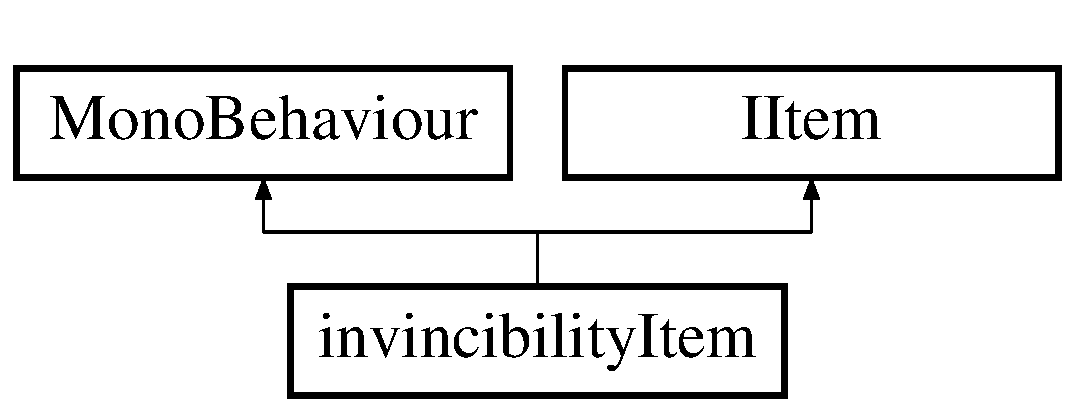
\includegraphics[height=2.000000cm]{classinvincibility_item}
\end{center}
\end{figure}
\subsection*{Public Member Functions}
\begin{DoxyCompactItemize}
\item 
void \mbox{\hyperlink{classinvincibility_item_a6fe1d452c0e956c50b4cb468b4bd140b}{Ability}} (\mbox{\hyperlink{class_i_player}{I\+Player}} player)
\item 
void \mbox{\hyperlink{classinvincibility_item_abe2368f3358065d15547f24e8cee2de5}{Duration}} (\mbox{\hyperlink{class_i_player}{I\+Player}} player)
\end{DoxyCompactItemize}


\subsection{Member Function Documentation}
\mbox{\Hypertarget{classinvincibility_item_a6fe1d452c0e956c50b4cb468b4bd140b}\label{classinvincibility_item_a6fe1d452c0e956c50b4cb468b4bd140b}} 
\index{invincibility\+Item@{invincibility\+Item}!Ability@{Ability}}
\index{Ability@{Ability}!invincibility\+Item@{invincibility\+Item}}
\subsubsection{\texorpdfstring{Ability()}{Ability()}}
{\footnotesize\ttfamily void invincibility\+Item.\+Ability (\begin{DoxyParamCaption}\item[{\mbox{\hyperlink{class_i_player}{I\+Player}}}]{player }\end{DoxyParamCaption})\hspace{0.3cm}{\ttfamily [inline]}}


\begin{DoxyParams}{Parameters}
{\em \mbox{\hyperlink{class_i_player}{I\+Player}}} & \\
\hline
\end{DoxyParams}
\begin{DoxyReturn}{Returns}
none Calls the ability of the item 
\end{DoxyReturn}


Implements \mbox{\hyperlink{interface_i_item_afe73efbf8316273df20162d6f4b20648}{I\+Item}}.

\mbox{\Hypertarget{classinvincibility_item_abe2368f3358065d15547f24e8cee2de5}\label{classinvincibility_item_abe2368f3358065d15547f24e8cee2de5}} 
\index{invincibility\+Item@{invincibility\+Item}!Duration@{Duration}}
\index{Duration@{Duration}!invincibility\+Item@{invincibility\+Item}}
\subsubsection{\texorpdfstring{Duration()}{Duration()}}
{\footnotesize\ttfamily void invincibility\+Item.\+Duration (\begin{DoxyParamCaption}\item[{\mbox{\hyperlink{class_i_player}{I\+Player}}}]{player }\end{DoxyParamCaption})\hspace{0.3cm}{\ttfamily [inline]}}


\begin{DoxyParams}{Parameters}
{\em \mbox{\hyperlink{class_i_player}{I\+Player}}} & \\
\hline
\end{DoxyParams}
\begin{DoxyReturn}{Returns}
none Sets the duration of the ability 
\end{DoxyReturn}


Implements \mbox{\hyperlink{interface_i_item_a797c1d62a7828bf428cc486ceaf18e9c}{I\+Item}}.



The documentation for this class was generated from the following file\+:\begin{DoxyCompactItemize}
\item 
invincibility\+Item.\+cs\end{DoxyCompactItemize}

\hypertarget{class_invincible_item_spawner}{}\section{Invincible\+Item\+Spawner Class Reference}
\label{class_invincible_item_spawner}\index{Invincible\+Item\+Spawner@{Invincible\+Item\+Spawner}}
Inheritance diagram for Invincible\+Item\+Spawner\+:\begin{figure}[H]
\begin{center}
\leavevmode
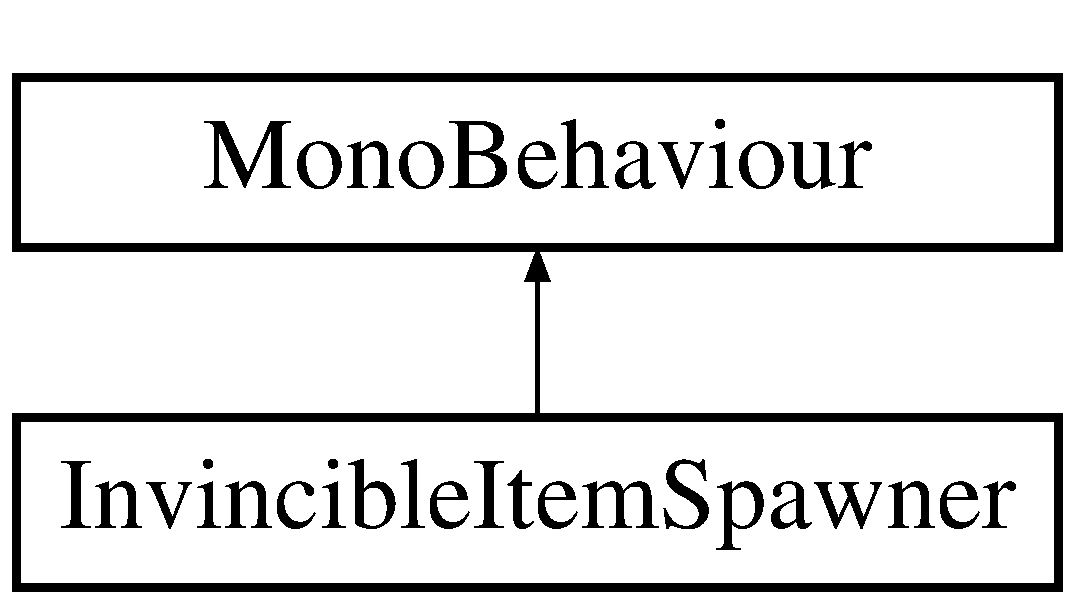
\includegraphics[height=2.000000cm]{class_invincible_item_spawner}
\end{center}
\end{figure}
\subsection*{Public Attributes}
\begin{DoxyCompactItemize}
\item 
\mbox{\Hypertarget{class_invincible_item_spawner_a9f165ee1f5eca266513a5c4d931fe889}\label{class_invincible_item_spawner_a9f165ee1f5eca266513a5c4d931fe889}} 
Game\+Object {\bfseries invincible\+Item}
\end{DoxyCompactItemize}


The documentation for this class was generated from the following file\+:\begin{DoxyCompactItemize}
\item 
Invincible\+Item\+Spawner.\+cs\end{DoxyCompactItemize}

\hypertarget{class_i_player}{}\section{I\+Player Class Reference}
\label{class_i_player}\index{I\+Player@{I\+Player}}
Inheritance diagram for I\+Player\+:\begin{figure}[H]
\begin{center}
\leavevmode
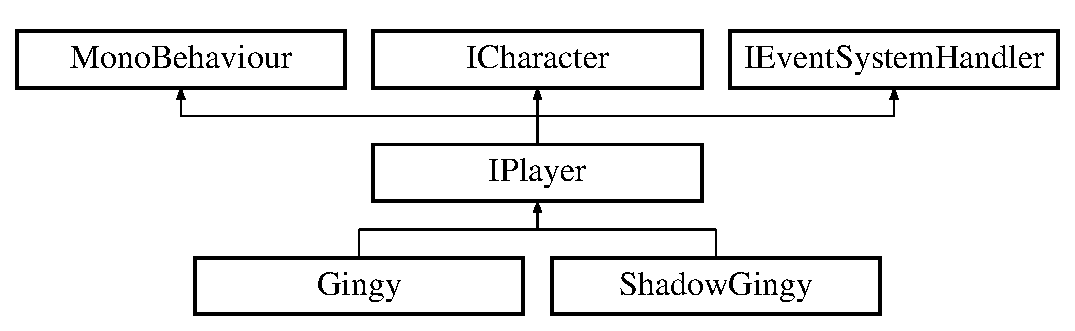
\includegraphics[height=3.000000cm]{class_i_player}
\end{center}
\end{figure}
\subsection*{Public Member Functions}
\begin{DoxyCompactItemize}
\item 
\mbox{\Hypertarget{class_i_player_a2053dee5dea8db35fe793024ea4d16a9}\label{class_i_player_a2053dee5dea8db35fe793024ea4d16a9}} 
void {\bfseries Start} ()
\item 
void \mbox{\hyperlink{class_i_player_a8a19883d426fa172adc043332426d7ec}{Take\+Damage}} (int damage\+Taken)
\item 
void \mbox{\hyperlink{class_i_player_a58a8e761b790450e9e190b3fdb5f2d29}{Attack}} ()
\item 
void \mbox{\hyperlink{class_i_player_a073e6b521b71c82a8e8d380ae991236f}{set\+Speed}} (int speed)
\item 
void \mbox{\hyperlink{class_i_player_a30143696c1b07bf382b8dac33cb7e6c1}{set\+Health}} (int health)
\item 
int \mbox{\hyperlink{class_i_player_a355f4da5d038c40df94194a2c545f526}{get\+Health}} ()
\item 
void \mbox{\hyperlink{class_i_player_ac5e448510f1d5c2b09ccd6e71aef57c8}{set\+Attack}} (int attack)
\item 
int \mbox{\hyperlink{class_i_player_aaf464871461953c9a35faac73a0d054f}{get\+Attack}} ()
\item 
void \mbox{\hyperlink{class_i_player_a2023f2ac17d8b79bb7f6d1830eca938f}{set\+Invincibility}} (bool invinc)
\item 
void \mbox{\hyperlink{class_i_player_a0a2ab5ba7ee4bfbba5e66f79315dd58c}{set\+I\+Duration}} (int dur)
\item 
int \mbox{\hyperlink{class_i_player_ad97d3469ea99b797926c1ec2c0b70c28}{get\+I\+Duration}} ()
\item 
void \mbox{\hyperlink{class_i_player_a3eaa74cff113c64a6cee96c9e0b3da5c}{set\+A\+Duration}} (int dur)
\item 
int \mbox{\hyperlink{class_i_player_a81cb512517a08129c77e730c114c5f98}{get\+A\+Duration}} ()
\item 
bool \mbox{\hyperlink{class_i_player_a4575d071d3465f3c0808232c222eb7cb}{is\+Dead}} ()
\item 
void \mbox{\hyperlink{class_i_player_a62499ee0288916e1220f64e18653c7b7}{Die}} ()
\end{DoxyCompactItemize}
\subsection*{Public Attributes}
\begin{DoxyCompactItemize}
\item 
\mbox{\Hypertarget{class_i_player_a52228afb290f3823a055ac7e1b62552f}\label{class_i_player_a52228afb290f3823a055ac7e1b62552f}} 
bool {\bfseries Invinc}
\item 
\mbox{\Hypertarget{class_i_player_a9f3c711426886a5386599b37c1e7987e}\label{class_i_player_a9f3c711426886a5386599b37c1e7987e}} 
int {\bfseries Invinc\+Dur}
\item 
\mbox{\Hypertarget{class_i_player_a4b8ca3067a4c9b973a01460be33a6aae}\label{class_i_player_a4b8ca3067a4c9b973a01460be33a6aae}} 
int {\bfseries Icount}
\item 
\mbox{\Hypertarget{class_i_player_a18da8ecdb8a63d0a93d75f6f59b719ef}\label{class_i_player_a18da8ecdb8a63d0a93d75f6f59b719ef}} 
int {\bfseries Attak}
\item 
\mbox{\Hypertarget{class_i_player_ace67debce789d1b103ae6f3c1d58561b}\label{class_i_player_ace67debce789d1b103ae6f3c1d58561b}} 
int {\bfseries Attak\+Dur}
\item 
\mbox{\Hypertarget{class_i_player_acd953caa4cbef2e580d8028a523036db}\label{class_i_player_acd953caa4cbef2e580d8028a523036db}} 
int {\bfseries Acount}
\item 
\mbox{\Hypertarget{class_i_player_a27e5fa4508d724dfc8c9e262a4e26ca1}\label{class_i_player_a27e5fa4508d724dfc8c9e262a4e26ca1}} 
int {\bfseries max\+Health} = 100
\item 
\mbox{\Hypertarget{class_i_player_a111ab23d1c1effff65699633e1508e6b}\label{class_i_player_a111ab23d1c1effff65699633e1508e6b}} 
string {\bfseries player\+Name}
\end{DoxyCompactItemize}
\subsection*{Static Public Attributes}
\begin{DoxyCompactItemize}
\item 
\mbox{\Hypertarget{class_i_player_a5357d5c2fcd3f36a79c32071432cdc44}\label{class_i_player_a5357d5c2fcd3f36a79c32071432cdc44}} 
static int {\bfseries Health}
\end{DoxyCompactItemize}


\subsection{Member Function Documentation}
\mbox{\Hypertarget{class_i_player_a58a8e761b790450e9e190b3fdb5f2d29}\label{class_i_player_a58a8e761b790450e9e190b3fdb5f2d29}} 
\index{I\+Player@{I\+Player}!Attack@{Attack}}
\index{Attack@{Attack}!I\+Player@{I\+Player}}
\subsubsection{\texorpdfstring{Attack()}{Attack()}}
{\footnotesize\ttfamily void I\+Player.\+Attack (\begin{DoxyParamCaption}{ }\end{DoxyParamCaption})\hspace{0.3cm}{\ttfamily [inline]}}

When the player attacks it determines if there is an enemy to do damage to or not  None  None 

Implements \mbox{\hyperlink{interface_i_character}{I\+Character}}.

\mbox{\Hypertarget{class_i_player_a62499ee0288916e1220f64e18653c7b7}\label{class_i_player_a62499ee0288916e1220f64e18653c7b7}} 
\index{I\+Player@{I\+Player}!Die@{Die}}
\index{Die@{Die}!I\+Player@{I\+Player}}
\subsubsection{\texorpdfstring{Die()}{Die()}}
{\footnotesize\ttfamily void I\+Player.\+Die (\begin{DoxyParamCaption}{ }\end{DoxyParamCaption})\hspace{0.3cm}{\ttfamily [inline]}}

Performs functions when player dies  None  none 

Implements \mbox{\hyperlink{interface_i_character_ad58356e457f98d8a6f9548da446012ce}{I\+Character}}.

\mbox{\Hypertarget{class_i_player_a81cb512517a08129c77e730c114c5f98}\label{class_i_player_a81cb512517a08129c77e730c114c5f98}} 
\index{I\+Player@{I\+Player}!get\+A\+Duration@{get\+A\+Duration}}
\index{get\+A\+Duration@{get\+A\+Duration}!I\+Player@{I\+Player}}
\subsubsection{\texorpdfstring{get\+A\+Duration()}{getADuration()}}
{\footnotesize\ttfamily int I\+Player.\+get\+A\+Duration (\begin{DoxyParamCaption}{ }\end{DoxyParamCaption})\hspace{0.3cm}{\ttfamily [inline]}}

Gets the attack item duration  None  int \mbox{\Hypertarget{class_i_player_aaf464871461953c9a35faac73a0d054f}\label{class_i_player_aaf464871461953c9a35faac73a0d054f}} 
\index{I\+Player@{I\+Player}!get\+Attack@{get\+Attack}}
\index{get\+Attack@{get\+Attack}!I\+Player@{I\+Player}}
\subsubsection{\texorpdfstring{get\+Attack()}{getAttack()}}
{\footnotesize\ttfamily int I\+Player.\+get\+Attack (\begin{DoxyParamCaption}{ }\end{DoxyParamCaption})\hspace{0.3cm}{\ttfamily [inline]}}

returns the attack of the player  None  Health \mbox{\Hypertarget{class_i_player_a355f4da5d038c40df94194a2c545f526}\label{class_i_player_a355f4da5d038c40df94194a2c545f526}} 
\index{I\+Player@{I\+Player}!get\+Health@{get\+Health}}
\index{get\+Health@{get\+Health}!I\+Player@{I\+Player}}
\subsubsection{\texorpdfstring{get\+Health()}{getHealth()}}
{\footnotesize\ttfamily int I\+Player.\+get\+Health (\begin{DoxyParamCaption}{ }\end{DoxyParamCaption})\hspace{0.3cm}{\ttfamily [inline]}}

Gets the health of the player  None  Health \mbox{\Hypertarget{class_i_player_ad97d3469ea99b797926c1ec2c0b70c28}\label{class_i_player_ad97d3469ea99b797926c1ec2c0b70c28}} 
\index{I\+Player@{I\+Player}!get\+I\+Duration@{get\+I\+Duration}}
\index{get\+I\+Duration@{get\+I\+Duration}!I\+Player@{I\+Player}}
\subsubsection{\texorpdfstring{get\+I\+Duration()}{getIDuration()}}
{\footnotesize\ttfamily int I\+Player.\+get\+I\+Duration (\begin{DoxyParamCaption}{ }\end{DoxyParamCaption})\hspace{0.3cm}{\ttfamily [inline]}}

gets the duration of the item  none  int \mbox{\Hypertarget{class_i_player_a4575d071d3465f3c0808232c222eb7cb}\label{class_i_player_a4575d071d3465f3c0808232c222eb7cb}} 
\index{I\+Player@{I\+Player}!is\+Dead@{is\+Dead}}
\index{is\+Dead@{is\+Dead}!I\+Player@{I\+Player}}
\subsubsection{\texorpdfstring{is\+Dead()}{isDead()}}
{\footnotesize\ttfamily bool I\+Player.\+is\+Dead (\begin{DoxyParamCaption}{ }\end{DoxyParamCaption})\hspace{0.3cm}{\ttfamily [inline]}}

sees if the player is dead  None  bool 

Implements \mbox{\hyperlink{interface_i_character}{I\+Character}}.

\mbox{\Hypertarget{class_i_player_a3eaa74cff113c64a6cee96c9e0b3da5c}\label{class_i_player_a3eaa74cff113c64a6cee96c9e0b3da5c}} 
\index{I\+Player@{I\+Player}!set\+A\+Duration@{set\+A\+Duration}}
\index{set\+A\+Duration@{set\+A\+Duration}!I\+Player@{I\+Player}}
\subsubsection{\texorpdfstring{set\+A\+Duration()}{setADuration()}}
{\footnotesize\ttfamily void I\+Player.\+set\+A\+Duration (\begin{DoxyParamCaption}\item[{int}]{dur }\end{DoxyParamCaption})\hspace{0.3cm}{\ttfamily [inline]}}

sets duration of the attack item  int  none \mbox{\Hypertarget{class_i_player_ac5e448510f1d5c2b09ccd6e71aef57c8}\label{class_i_player_ac5e448510f1d5c2b09ccd6e71aef57c8}} 
\index{I\+Player@{I\+Player}!set\+Attack@{set\+Attack}}
\index{set\+Attack@{set\+Attack}!I\+Player@{I\+Player}}
\subsubsection{\texorpdfstring{set\+Attack()}{setAttack()}}
{\footnotesize\ttfamily void I\+Player.\+set\+Attack (\begin{DoxyParamCaption}\item[{int}]{attack }\end{DoxyParamCaption})\hspace{0.3cm}{\ttfamily [inline]}}

sets attack of the player  int  none \mbox{\Hypertarget{class_i_player_a30143696c1b07bf382b8dac33cb7e6c1}\label{class_i_player_a30143696c1b07bf382b8dac33cb7e6c1}} 
\index{I\+Player@{I\+Player}!set\+Health@{set\+Health}}
\index{set\+Health@{set\+Health}!I\+Player@{I\+Player}}
\subsubsection{\texorpdfstring{set\+Health()}{setHealth()}}
{\footnotesize\ttfamily void I\+Player.\+set\+Health (\begin{DoxyParamCaption}\item[{int}]{health }\end{DoxyParamCaption})\hspace{0.3cm}{\ttfamily [inline]}}

Sets the health for the player  int health  None 

Implements \mbox{\hyperlink{interface_i_character}{I\+Character}}.

\mbox{\Hypertarget{class_i_player_a0a2ab5ba7ee4bfbba5e66f79315dd58c}\label{class_i_player_a0a2ab5ba7ee4bfbba5e66f79315dd58c}} 
\index{I\+Player@{I\+Player}!set\+I\+Duration@{set\+I\+Duration}}
\index{set\+I\+Duration@{set\+I\+Duration}!I\+Player@{I\+Player}}
\subsubsection{\texorpdfstring{set\+I\+Duration()}{setIDuration()}}
{\footnotesize\ttfamily void I\+Player.\+set\+I\+Duration (\begin{DoxyParamCaption}\item[{int}]{dur }\end{DoxyParamCaption})\hspace{0.3cm}{\ttfamily [inline]}}

sets the duration of the item picked up  int  none \mbox{\Hypertarget{class_i_player_a2023f2ac17d8b79bb7f6d1830eca938f}\label{class_i_player_a2023f2ac17d8b79bb7f6d1830eca938f}} 
\index{I\+Player@{I\+Player}!set\+Invincibility@{set\+Invincibility}}
\index{set\+Invincibility@{set\+Invincibility}!I\+Player@{I\+Player}}
\subsubsection{\texorpdfstring{set\+Invincibility()}{setInvincibility()}}
{\footnotesize\ttfamily void I\+Player.\+set\+Invincibility (\begin{DoxyParamCaption}\item[{bool}]{invinc }\end{DoxyParamCaption})\hspace{0.3cm}{\ttfamily [inline]}}

set\+Invincibility  bool  none \mbox{\Hypertarget{class_i_player_a073e6b521b71c82a8e8d380ae991236f}\label{class_i_player_a073e6b521b71c82a8e8d380ae991236f}} 
\index{I\+Player@{I\+Player}!set\+Speed@{set\+Speed}}
\index{set\+Speed@{set\+Speed}!I\+Player@{I\+Player}}
\subsubsection{\texorpdfstring{set\+Speed()}{setSpeed()}}
{\footnotesize\ttfamily void I\+Player.\+set\+Speed (\begin{DoxyParamCaption}\item[{int}]{speed }\end{DoxyParamCaption})\hspace{0.3cm}{\ttfamily [inline]}}

void  int speed  None 

Implements \mbox{\hyperlink{interface_i_character}{I\+Character}}.

\mbox{\Hypertarget{class_i_player_a8a19883d426fa172adc043332426d7ec}\label{class_i_player_a8a19883d426fa172adc043332426d7ec}} 
\index{I\+Player@{I\+Player}!Take\+Damage@{Take\+Damage}}
\index{Take\+Damage@{Take\+Damage}!I\+Player@{I\+Player}}
\subsubsection{\texorpdfstring{Take\+Damage()}{TakeDamage()}}
{\footnotesize\ttfamily void I\+Player.\+Take\+Damage (\begin{DoxyParamCaption}\item[{int}]{damage\+Taken }\end{DoxyParamCaption})\hspace{0.3cm}{\ttfamily [inline]}}

Takes Damage given to the character  int damage\+Taken  None 

Implements \mbox{\hyperlink{interface_i_character}{I\+Character}}.



The documentation for this class was generated from the following file\+:\begin{DoxyCompactItemize}
\item 
I\+Player.\+cs\end{DoxyCompactItemize}

\hypertarget{interface_i_test_event_system}{}\section{I\+Test\+Event\+System Interface Reference}
\label{interface_i_test_event_system}\index{I\+Test\+Event\+System@{I\+Test\+Event\+System}}
Inheritance diagram for I\+Test\+Event\+System\+:\begin{figure}[H]
\begin{center}
\leavevmode
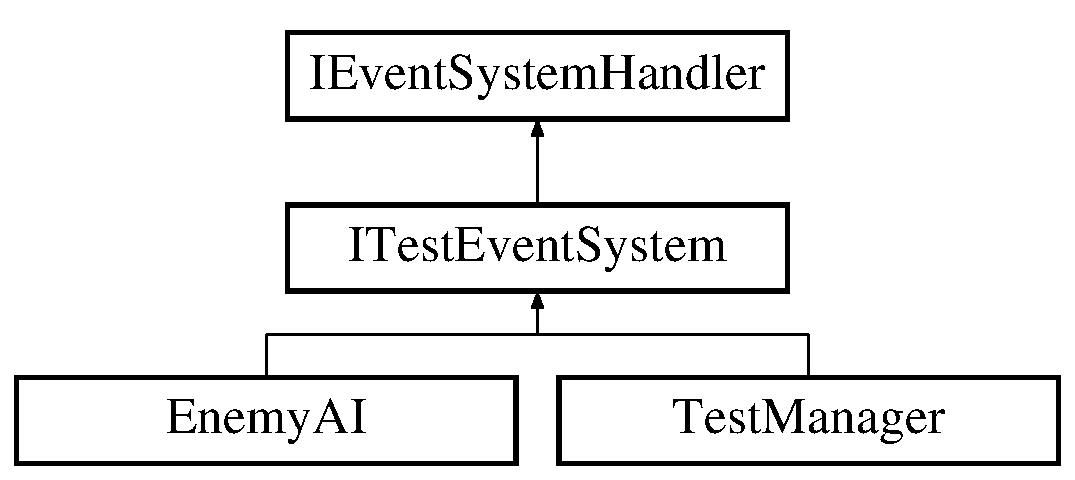
\includegraphics[height=3.000000cm]{interface_i_test_event_system}
\end{center}
\end{figure}
\subsection*{Public Member Functions}
\begin{DoxyCompactItemize}
\item 
void \mbox{\hyperlink{interface_i_test_event_system_aefeb7857cc94ecb2bacb47975f6474bb}{Start\+Test}} ()
\item 
void \mbox{\hyperlink{interface_i_test_event_system_ae8eda94179d81c4c839a32432216df7b}{End\+Test}} ()
\end{DoxyCompactItemize}


\subsection{Member Function Documentation}
\mbox{\Hypertarget{interface_i_test_event_system_ae8eda94179d81c4c839a32432216df7b}\label{interface_i_test_event_system_ae8eda94179d81c4c839a32432216df7b}} 
\index{I\+Test\+Event\+System@{I\+Test\+Event\+System}!End\+Test@{End\+Test}}
\index{End\+Test@{End\+Test}!I\+Test\+Event\+System@{I\+Test\+Event\+System}}
\subsubsection{\texorpdfstring{End\+Test()}{EndTest()}}
{\footnotesize\ttfamily void I\+Test\+Event\+System.\+End\+Test (\begin{DoxyParamCaption}{ }\end{DoxyParamCaption})}


\begin{DoxyParams}{Parameters}
{\em none} & \\
\hline
\end{DoxyParams}
\begin{DoxyReturn}{Returns}
none Use of the eventsystemhandler to message end test 
\end{DoxyReturn}


Implemented in \mbox{\hyperlink{class_enemy_a_i_a63dc8e816322f34ec0360a1189fb931e}{Enemy\+AI}}, and \mbox{\hyperlink{class_test_manager_a39a04c0d50c7be1322ad25e67696e549}{Test\+Manager}}.

\mbox{\Hypertarget{interface_i_test_event_system_aefeb7857cc94ecb2bacb47975f6474bb}\label{interface_i_test_event_system_aefeb7857cc94ecb2bacb47975f6474bb}} 
\index{I\+Test\+Event\+System@{I\+Test\+Event\+System}!Start\+Test@{Start\+Test}}
\index{Start\+Test@{Start\+Test}!I\+Test\+Event\+System@{I\+Test\+Event\+System}}
\subsubsection{\texorpdfstring{Start\+Test()}{StartTest()}}
{\footnotesize\ttfamily void I\+Test\+Event\+System.\+Start\+Test (\begin{DoxyParamCaption}{ }\end{DoxyParamCaption})}


\begin{DoxyParams}{Parameters}
{\em none} & \\
\hline
\end{DoxyParams}
\begin{DoxyReturn}{Returns}
none Use of the eventsystemhandler to message start test 
\end{DoxyReturn}


Implemented in \mbox{\hyperlink{class_enemy_a_i_a8d23dd153a4f273abaae5c174d10a6d2}{Enemy\+AI}}, and \mbox{\hyperlink{class_test_manager_a74fe528d0e18c4cca484bca002dc4f2b}{Test\+Manager}}.



The documentation for this interface was generated from the following file\+:\begin{DoxyCompactItemize}
\item 
I\+Test\+Event\+System.\+cs\end{DoxyCompactItemize}

\hypertarget{class_jack}{}\section{Jack Class Reference}
\label{class_jack}\index{Jack@{Jack}}
Inheritance diagram for Jack\+:\begin{figure}[H]
\begin{center}
\leavevmode
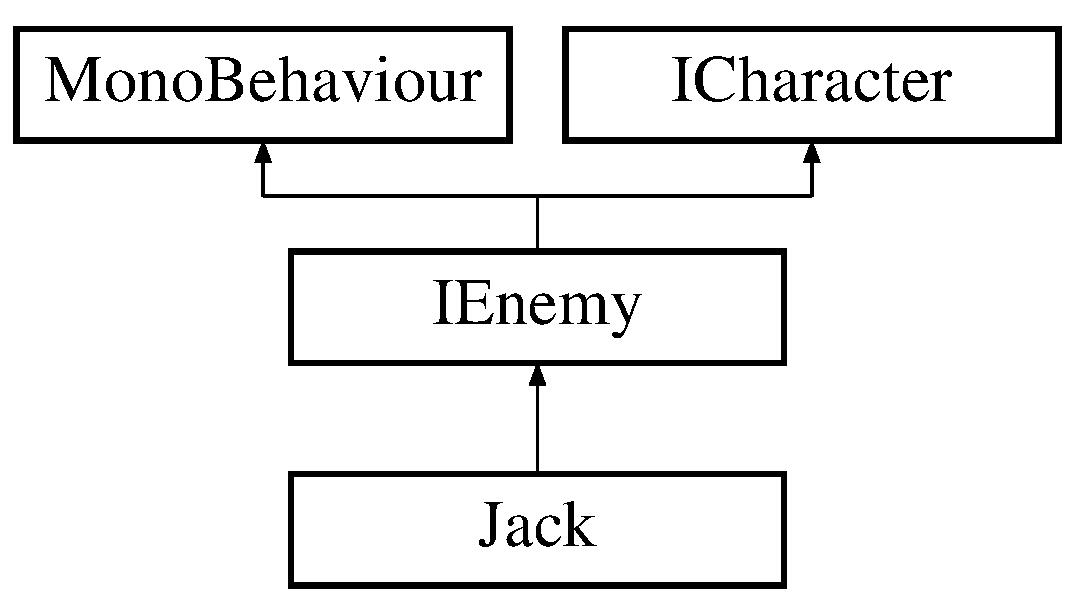
\includegraphics[height=3.000000cm]{class_jack}
\end{center}
\end{figure}
\subsection*{Public Member Functions}
\begin{DoxyCompactItemize}
\item 
void \mbox{\hyperlink{class_jack_a5c422cd6a8147746decbfe4b9843f469}{Set\+Move}} (bool value)
\item 
void \mbox{\hyperlink{class_jack_aba39628731cb774d63414f8b0702794b}{Fixed\+Update}} ()
\item 
void \mbox{\hyperlink{class_jack_af6f345fe0fa0b4d3633b671d31d0d76e}{Take\+Damage}} (int damage\+Taken)
\item 
void \mbox{\hyperlink{class_jack_a5c58f59b2bd9197a006a3e4739cc4503}{Attack}} ()
\item 
void \mbox{\hyperlink{class_jack_a9ae28ec3e59646a7f5cdd7a2fcf58a20}{set\+Speed}} (int speed)
\item 
void \mbox{\hyperlink{class_jack_a8d41ae6c0691bcc01910758e106e29cf}{set\+Health}} (int health)
\item 
bool \mbox{\hyperlink{class_jack_a50b5fbbb94e899db67599a763f9e687b}{is\+Dead}} ()
\end{DoxyCompactItemize}
\subsection*{Public Attributes}
\begin{DoxyCompactItemize}
\item 
\mbox{\Hypertarget{class_jack_ae497d5554be7cf372f934a2b024a4cfd}\label{class_jack_ae497d5554be7cf372f934a2b024a4cfd}} 
Vector3 {\bfseries current}
\item 
\mbox{\Hypertarget{class_jack_af0433564aed144c46d99ecc20518b501}\label{class_jack_af0433564aed144c46d99ecc20518b501}} 
Vector3 {\bfseries target}
\end{DoxyCompactItemize}


\subsection{Member Function Documentation}
\mbox{\Hypertarget{class_jack_a5c58f59b2bd9197a006a3e4739cc4503}\label{class_jack_a5c58f59b2bd9197a006a3e4739cc4503}} 
\index{Jack@{Jack}!Attack@{Attack}}
\index{Attack@{Attack}!Jack@{Jack}}
\subsubsection{\texorpdfstring{Attack()}{Attack()}}
{\footnotesize\ttfamily void Jack.\+Attack (\begin{DoxyParamCaption}{ }\end{DoxyParamCaption})\hspace{0.3cm}{\ttfamily [inline]}}

Attack 
\begin{DoxyParams}{Parameters}
{\em none} & \\
\hline
\end{DoxyParams}
\begin{DoxyReturn}{Returns}
none attack animation for player 
\end{DoxyReturn}
Attack Left ////

Attack Up ////

Attack Down //// 

Implements \mbox{\hyperlink{interface_i_character}{I\+Character}}.

\mbox{\Hypertarget{class_jack_aba39628731cb774d63414f8b0702794b}\label{class_jack_aba39628731cb774d63414f8b0702794b}} 
\index{Jack@{Jack}!Fixed\+Update@{Fixed\+Update}}
\index{Fixed\+Update@{Fixed\+Update}!Jack@{Jack}}
\subsubsection{\texorpdfstring{Fixed\+Update()}{FixedUpdate()}}
{\footnotesize\ttfamily void Jack.\+Fixed\+Update (\begin{DoxyParamCaption}{ }\end{DoxyParamCaption})\hspace{0.3cm}{\ttfamily [inline]}}

Fixed\+Update 
\begin{DoxyParams}{Parameters}
{\em none} & \\
\hline
\end{DoxyParams}
\begin{DoxyReturn}{Returns}
none Called every .02 sec 
\end{DoxyReturn}
\mbox{\Hypertarget{class_jack_a50b5fbbb94e899db67599a763f9e687b}\label{class_jack_a50b5fbbb94e899db67599a763f9e687b}} 
\index{Jack@{Jack}!is\+Dead@{is\+Dead}}
\index{is\+Dead@{is\+Dead}!Jack@{Jack}}
\subsubsection{\texorpdfstring{is\+Dead()}{isDead()}}
{\footnotesize\ttfamily bool Jack.\+is\+Dead (\begin{DoxyParamCaption}{ }\end{DoxyParamCaption})\hspace{0.3cm}{\ttfamily [inline]}}

is\+Dead 
\begin{DoxyParams}{Parameters}
{\em none} & \\
\hline
\end{DoxyParams}
\begin{DoxyReturn}{Returns}
bool Checks to see if character is dead 
\end{DoxyReturn}


Implements \mbox{\hyperlink{interface_i_character}{I\+Character}}.

\mbox{\Hypertarget{class_jack_a8d41ae6c0691bcc01910758e106e29cf}\label{class_jack_a8d41ae6c0691bcc01910758e106e29cf}} 
\index{Jack@{Jack}!set\+Health@{set\+Health}}
\index{set\+Health@{set\+Health}!Jack@{Jack}}
\subsubsection{\texorpdfstring{set\+Health()}{setHealth()}}
{\footnotesize\ttfamily void Jack.\+set\+Health (\begin{DoxyParamCaption}\item[{int}]{health }\end{DoxyParamCaption})\hspace{0.3cm}{\ttfamily [inline]}}

set\+Health 
\begin{DoxyParams}{Parameters}
{\em int} & \\
\hline
\end{DoxyParams}
\begin{DoxyReturn}{Returns}
none void 
\end{DoxyReturn}


Implements \mbox{\hyperlink{interface_i_character}{I\+Character}}.

\mbox{\Hypertarget{class_jack_a5c422cd6a8147746decbfe4b9843f469}\label{class_jack_a5c422cd6a8147746decbfe4b9843f469}} 
\index{Jack@{Jack}!Set\+Move@{Set\+Move}}
\index{Set\+Move@{Set\+Move}!Jack@{Jack}}
\subsubsection{\texorpdfstring{Set\+Move()}{SetMove()}}
{\footnotesize\ttfamily void Jack.\+Set\+Move (\begin{DoxyParamCaption}\item[{bool}]{value }\end{DoxyParamCaption})\hspace{0.3cm}{\ttfamily [inline]}}

Set\+Move 
\begin{DoxyParams}{Parameters}
{\em bool} & \\
\hline
\end{DoxyParams}
\begin{DoxyReturn}{Returns}
none Sets the value of move to input value 
\end{DoxyReturn}
\mbox{\Hypertarget{class_jack_a9ae28ec3e59646a7f5cdd7a2fcf58a20}\label{class_jack_a9ae28ec3e59646a7f5cdd7a2fcf58a20}} 
\index{Jack@{Jack}!set\+Speed@{set\+Speed}}
\index{set\+Speed@{set\+Speed}!Jack@{Jack}}
\subsubsection{\texorpdfstring{set\+Speed()}{setSpeed()}}
{\footnotesize\ttfamily void Jack.\+set\+Speed (\begin{DoxyParamCaption}\item[{int}]{speed }\end{DoxyParamCaption})\hspace{0.3cm}{\ttfamily [inline]}}

set\+Speed 
\begin{DoxyParams}{Parameters}
{\em int} & \\
\hline
\end{DoxyParams}
\begin{DoxyReturn}{Returns}
none void 
\end{DoxyReturn}


Implements \mbox{\hyperlink{interface_i_character}{I\+Character}}.

\mbox{\Hypertarget{class_jack_af6f345fe0fa0b4d3633b671d31d0d76e}\label{class_jack_af6f345fe0fa0b4d3633b671d31d0d76e}} 
\index{Jack@{Jack}!Take\+Damage@{Take\+Damage}}
\index{Take\+Damage@{Take\+Damage}!Jack@{Jack}}
\subsubsection{\texorpdfstring{Take\+Damage()}{TakeDamage()}}
{\footnotesize\ttfamily void Jack.\+Take\+Damage (\begin{DoxyParamCaption}\item[{int}]{damage\+Taken }\end{DoxyParamCaption})\hspace{0.3cm}{\ttfamily [inline]}}

Take\+Damage 
\begin{DoxyParams}{Parameters}
{\em int} & \\
\hline
\end{DoxyParams}
\begin{DoxyReturn}{Returns}
none Reduces health of gameobject 
\end{DoxyReturn}


Implements \mbox{\hyperlink{interface_i_character}{I\+Character}}.



The documentation for this class was generated from the following file\+:\begin{DoxyCompactItemize}
\item 
Jack.\+cs\end{DoxyCompactItemize}

\hypertarget{class_jack_spawner}{}\section{Jack\+Spawner Class Reference}
\label{class_jack_spawner}\index{Jack\+Spawner@{Jack\+Spawner}}
Inheritance diagram for Jack\+Spawner\+:\begin{figure}[H]
\begin{center}
\leavevmode
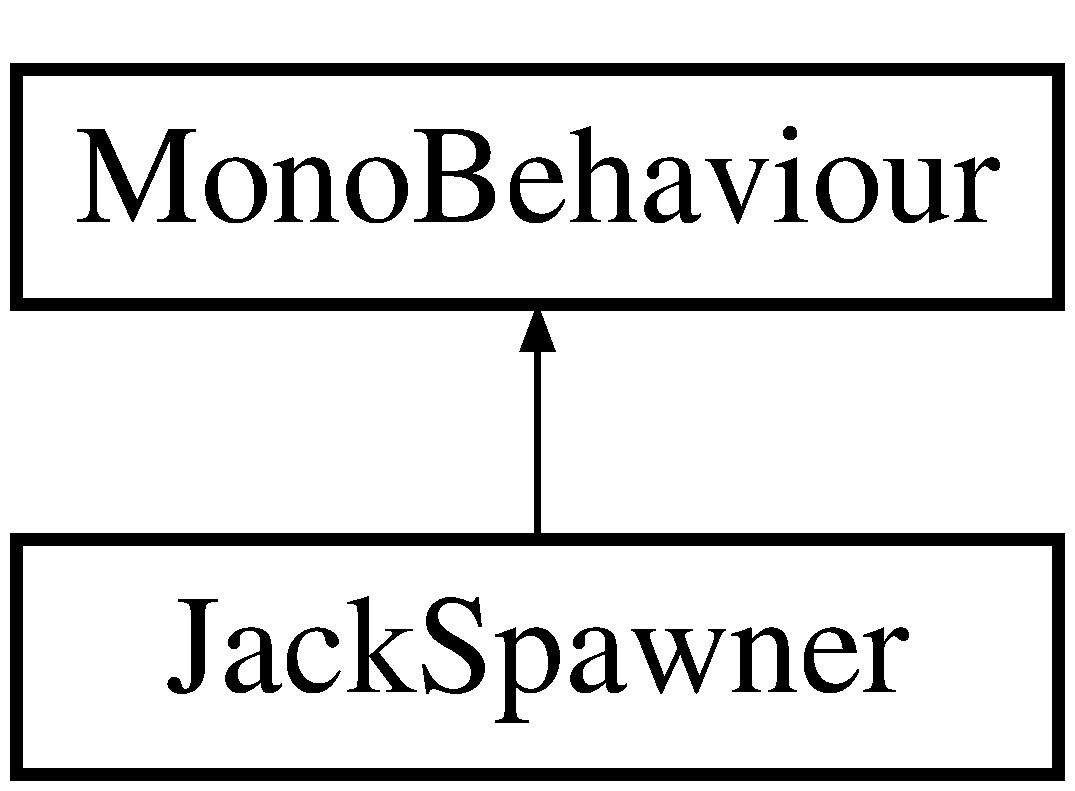
\includegraphics[height=2.000000cm]{class_jack_spawner}
\end{center}
\end{figure}
\subsection*{Public Attributes}
\begin{DoxyCompactItemize}
\item 
\mbox{\Hypertarget{class_jack_spawner_a420c4754b81618c823f9dfbeb5b1d0e9}\label{class_jack_spawner_a420c4754b81618c823f9dfbeb5b1d0e9}} 
Game\+Object {\bfseries jack}
\end{DoxyCompactItemize}


The documentation for this class was generated from the following file\+:\begin{DoxyCompactItemize}
\item 
Jack\+Spawner.\+cs\end{DoxyCompactItemize}

\hypertarget{class_completed_1_1_level_generator}{}\section{Completed.\+Level\+Generator Class Reference}
\label{class_completed_1_1_level_generator}\index{Completed.\+Level\+Generator@{Completed.\+Level\+Generator}}
Inheritance diagram for Completed.\+Level\+Generator\+:\begin{figure}[H]
\begin{center}
\leavevmode
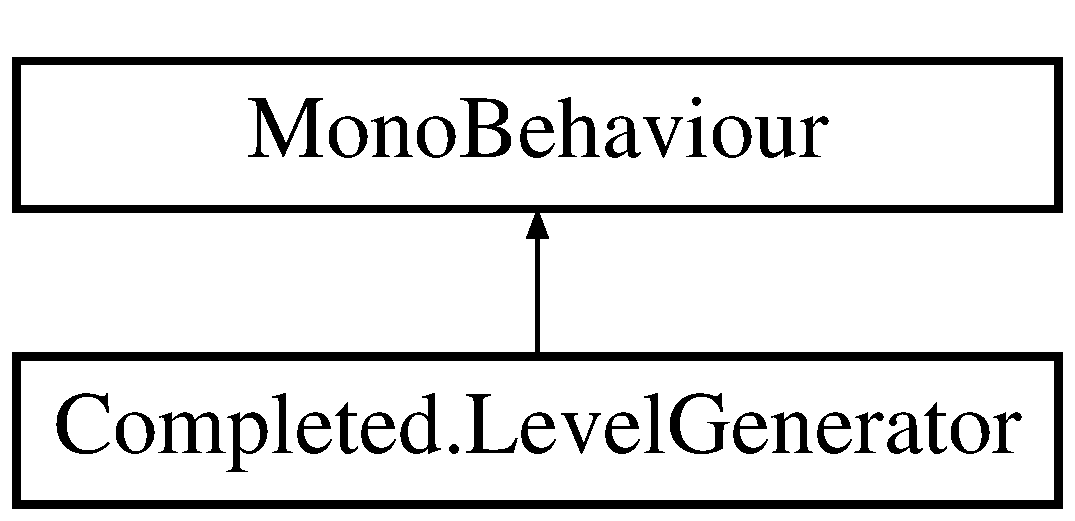
\includegraphics[height=2.000000cm]{class_completed_1_1_level_generator}
\end{center}
\end{figure}
\subsection*{Public Member Functions}
\begin{DoxyCompactItemize}
\item 
void \mbox{\hyperlink{class_completed_1_1_level_generator_a1c8e4f88ea8b0667f9270e5ec4224d01}{Setup\+Scene}} (int level, Game\+Object Player)
\item 
int \mbox{\hyperlink{class_completed_1_1_level_generator_a2ffea5be00328c47fa5460db2386b8e5}{get\+Num\+Enemies}} ()
\item 
void \mbox{\hyperlink{class_completed_1_1_level_generator_a2b17e9d80d8ad66ee1c45234eb3fd47c}{Clear\+Map}} ()
\end{DoxyCompactItemize}
\subsection*{Public Attributes}
\begin{DoxyCompactItemize}
\item 
\mbox{\Hypertarget{class_completed_1_1_level_generator_a1f495bac99f2520a6cdc7949abd1901a}\label{class_completed_1_1_level_generator_a1f495bac99f2520a6cdc7949abd1901a}} 
int {\bfseries placed\+Floors}
\item 
\mbox{\Hypertarget{class_completed_1_1_level_generator_a4d3a79f611c1f1958372a9fa018fef12}\label{class_completed_1_1_level_generator_a4d3a79f611c1f1958372a9fa018fef12}} 
int {\bfseries num\+Floor\+Tiles}
\item 
\mbox{\Hypertarget{class_completed_1_1_level_generator_a3683acf37342e58917d62bdfb4920605}\label{class_completed_1_1_level_generator_a3683acf37342e58917d62bdfb4920605}} 
\mbox{\hyperlink{class_map}{Map}} {\bfseries map}
\item 
\mbox{\Hypertarget{class_completed_1_1_level_generator_a96a5d7a791a7cace1db5fac4932bd0a3}\label{class_completed_1_1_level_generator_a96a5d7a791a7cace1db5fac4932bd0a3}} 
int {\bfseries num\+Items}
\item 
\mbox{\Hypertarget{class_completed_1_1_level_generator_a285945bcaa4e52d34b86ffc0c5492d60}\label{class_completed_1_1_level_generator_a285945bcaa4e52d34b86ffc0c5492d60}} 
Game\+Object \mbox{[}$\,$\mbox{]} {\bfseries Items}
\item 
\mbox{\Hypertarget{class_completed_1_1_level_generator_ab820dfc29b9b876659a155b7e72dcc15}\label{class_completed_1_1_level_generator_ab820dfc29b9b876659a155b7e72dcc15}} 
Vector3 {\bfseries player\+Pos}
\item 
\mbox{\Hypertarget{class_completed_1_1_level_generator_af03eb9a29d8b0625e56d72f6e518cacf}\label{class_completed_1_1_level_generator_af03eb9a29d8b0625e56d72f6e518cacf}} 
Game\+Object {\bfseries Enemy1}
\item 
\mbox{\Hypertarget{class_completed_1_1_level_generator_ae4eae8507c2cf1f189e4ebea5f0eb583}\label{class_completed_1_1_level_generator_ae4eae8507c2cf1f189e4ebea5f0eb583}} 
Game\+Object {\bfseries Enemy2}
\item 
\mbox{\Hypertarget{class_completed_1_1_level_generator_ab86a3e3ed35bf6e2e9982ace6efd3fb2}\label{class_completed_1_1_level_generator_ab86a3e3ed35bf6e2e9982ace6efd3fb2}} 
List$<$ Vector3 $>$ {\bfseries enemy\+Positions}
\item 
\mbox{\Hypertarget{class_completed_1_1_level_generator_acb8af6a600d1121e4d1e55c8b827d4ff}\label{class_completed_1_1_level_generator_acb8af6a600d1121e4d1e55c8b827d4ff}} 
int {\bfseries num\+Enemies}
\item 
\mbox{\Hypertarget{class_completed_1_1_level_generator_a40be5987bfeab713d13ba240cdabb3c2}\label{class_completed_1_1_level_generator_a40be5987bfeab713d13ba240cdabb3c2}} 
int {\bfseries my\+Level}
\end{DoxyCompactItemize}


\subsection{Member Function Documentation}
\mbox{\Hypertarget{class_completed_1_1_level_generator_a2b17e9d80d8ad66ee1c45234eb3fd47c}\label{class_completed_1_1_level_generator_a2b17e9d80d8ad66ee1c45234eb3fd47c}} 
\index{Completed\+::\+Level\+Generator@{Completed\+::\+Level\+Generator}!Clear\+Map@{Clear\+Map}}
\index{Clear\+Map@{Clear\+Map}!Completed\+::\+Level\+Generator@{Completed\+::\+Level\+Generator}}
\subsubsection{\texorpdfstring{Clear\+Map()}{ClearMap()}}
{\footnotesize\ttfamily void Completed.\+Level\+Generator.\+Clear\+Map (\begin{DoxyParamCaption}{ }\end{DoxyParamCaption})\hspace{0.3cm}{\ttfamily [inline]}}


\begin{DoxyParams}{Parameters}
{\em none} & \\
\hline
\end{DoxyParams}
\begin{DoxyReturn}{Returns}
none Clears the entire map 
\end{DoxyReturn}
\mbox{\Hypertarget{class_completed_1_1_level_generator_a2ffea5be00328c47fa5460db2386b8e5}\label{class_completed_1_1_level_generator_a2ffea5be00328c47fa5460db2386b8e5}} 
\index{Completed\+::\+Level\+Generator@{Completed\+::\+Level\+Generator}!get\+Num\+Enemies@{get\+Num\+Enemies}}
\index{get\+Num\+Enemies@{get\+Num\+Enemies}!Completed\+::\+Level\+Generator@{Completed\+::\+Level\+Generator}}
\subsubsection{\texorpdfstring{get\+Num\+Enemies()}{getNumEnemies()}}
{\footnotesize\ttfamily int Completed.\+Level\+Generator.\+get\+Num\+Enemies (\begin{DoxyParamCaption}{ }\end{DoxyParamCaption})\hspace{0.3cm}{\ttfamily [inline]}}


\begin{DoxyParams}{Parameters}
{\em none} & \\
\hline
\end{DoxyParams}
\begin{DoxyReturn}{Returns}
int returns the number of enemies remaining 
\end{DoxyReturn}
\mbox{\Hypertarget{class_completed_1_1_level_generator_a1c8e4f88ea8b0667f9270e5ec4224d01}\label{class_completed_1_1_level_generator_a1c8e4f88ea8b0667f9270e5ec4224d01}} 
\index{Completed\+::\+Level\+Generator@{Completed\+::\+Level\+Generator}!Setup\+Scene@{Setup\+Scene}}
\index{Setup\+Scene@{Setup\+Scene}!Completed\+::\+Level\+Generator@{Completed\+::\+Level\+Generator}}
\subsubsection{\texorpdfstring{Setup\+Scene()}{SetupScene()}}
{\footnotesize\ttfamily void Completed.\+Level\+Generator.\+Setup\+Scene (\begin{DoxyParamCaption}\item[{int}]{level,  }\item[{Game\+Object}]{Player }\end{DoxyParamCaption})\hspace{0.3cm}{\ttfamily [inline]}}


\begin{DoxyParams}{Parameters}
{\em int} & level \\
\hline
\end{DoxyParams}
\begin{DoxyReturn}{Returns}
none Main function of \mbox{\hyperlink{class_completed_1_1_level_generator}{Level\+Generator}} Responsible for calling all other functions that setup the map 
\end{DoxyReturn}


The documentation for this class was generated from the following file\+:\begin{DoxyCompactItemize}
\item 
Level\+Generator.\+cs\end{DoxyCompactItemize}

\hypertarget{class_level_manager}{}\section{Level\+Manager Class Reference}
\label{class_level_manager}\index{Level\+Manager@{Level\+Manager}}
Inheritance diagram for Level\+Manager\+:\begin{figure}[H]
\begin{center}
\leavevmode
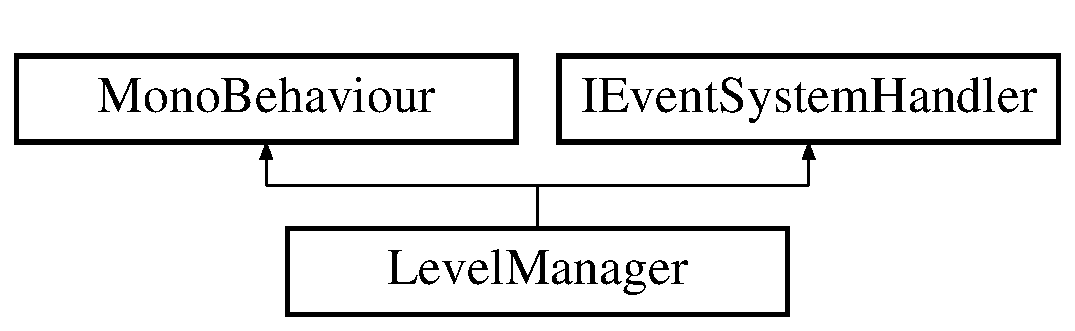
\includegraphics[height=2.000000cm]{class_level_manager}
\end{center}
\end{figure}
\subsection*{Public Member Functions}
\begin{DoxyCompactItemize}
\item 
void \mbox{\hyperlink{class_level_manager_a3f1b65f6b95299d86c615c9722f5da10}{start\+Level}} (int level, Game\+Object character)
\item 
int \mbox{\hyperlink{class_level_manager_a2b4501007dcaaa1df85ff558887f59f8}{get\+Num\+Enemies}} ()
\item 
bool \mbox{\hyperlink{class_level_manager_a28ffd8fcec835f1c04c8013c1173834a}{is\+Level\+Over}} ()
\end{DoxyCompactItemize}
\subsection*{Public Attributes}
\begin{DoxyCompactItemize}
\item 
\mbox{\Hypertarget{class_level_manager_a2d9c37e6a44b5deccece48f80aaec88e}\label{class_level_manager_a2d9c37e6a44b5deccece48f80aaec88e}} 
\mbox{\hyperlink{class_completed_1_1_level_generator}{Level\+Generator}} {\bfseries level\+Generator}
\item 
\mbox{\Hypertarget{class_level_manager_a376391b9d38d7ed131a528ce7d216855}\label{class_level_manager_a376391b9d38d7ed131a528ce7d216855}} 
Game\+Object {\bfseries main\+Character}
\end{DoxyCompactItemize}


\subsection{Member Function Documentation}
\mbox{\Hypertarget{class_level_manager_a2b4501007dcaaa1df85ff558887f59f8}\label{class_level_manager_a2b4501007dcaaa1df85ff558887f59f8}} 
\index{Level\+Manager@{Level\+Manager}!get\+Num\+Enemies@{get\+Num\+Enemies}}
\index{get\+Num\+Enemies@{get\+Num\+Enemies}!Level\+Manager@{Level\+Manager}}
\subsubsection{\texorpdfstring{get\+Num\+Enemies()}{getNumEnemies()}}
{\footnotesize\ttfamily int Level\+Manager.\+get\+Num\+Enemies (\begin{DoxyParamCaption}{ }\end{DoxyParamCaption})\hspace{0.3cm}{\ttfamily [inline]}}


\begin{DoxyParams}{Parameters}
{\em none} & \\
\hline
\end{DoxyParams}
\begin{DoxyReturn}{Returns}
int returns the number of enemies from level\+Generator 
\end{DoxyReturn}
\mbox{\Hypertarget{class_level_manager_a28ffd8fcec835f1c04c8013c1173834a}\label{class_level_manager_a28ffd8fcec835f1c04c8013c1173834a}} 
\index{Level\+Manager@{Level\+Manager}!is\+Level\+Over@{is\+Level\+Over}}
\index{is\+Level\+Over@{is\+Level\+Over}!Level\+Manager@{Level\+Manager}}
\subsubsection{\texorpdfstring{is\+Level\+Over()}{isLevelOver()}}
{\footnotesize\ttfamily bool Level\+Manager.\+is\+Level\+Over (\begin{DoxyParamCaption}{ }\end{DoxyParamCaption})\hspace{0.3cm}{\ttfamily [inline]}}


\begin{DoxyParams}{Parameters}
{\em none} & \\
\hline
\end{DoxyParams}
\begin{DoxyReturn}{Returns}
bool Checks to see fi the number of enemies is 0 true if there are no enemies, false otherwise 
\end{DoxyReturn}
\mbox{\Hypertarget{class_level_manager_a3f1b65f6b95299d86c615c9722f5da10}\label{class_level_manager_a3f1b65f6b95299d86c615c9722f5da10}} 
\index{Level\+Manager@{Level\+Manager}!start\+Level@{start\+Level}}
\index{start\+Level@{start\+Level}!Level\+Manager@{Level\+Manager}}
\subsubsection{\texorpdfstring{start\+Level()}{startLevel()}}
{\footnotesize\ttfamily void Level\+Manager.\+start\+Level (\begin{DoxyParamCaption}\item[{int}]{level,  }\item[{Game\+Object}]{character }\end{DoxyParamCaption})\hspace{0.3cm}{\ttfamily [inline]}}


\begin{DoxyParams}{Parameters}
{\em int} & level, Game\+Object character \\
\hline
\end{DoxyParams}
\begin{DoxyReturn}{Returns}
none Starts the level by placing player and setting up scene 
\end{DoxyReturn}


The documentation for this class was generated from the following file\+:\begin{DoxyCompactItemize}
\item 
Level\+Manager.\+cs\end{DoxyCompactItemize}

\hypertarget{class_loader}{}\section{Loader Class Reference}
\label{class_loader}\index{Loader@{Loader}}
Inheritance diagram for Loader\+:\begin{figure}[H]
\begin{center}
\leavevmode
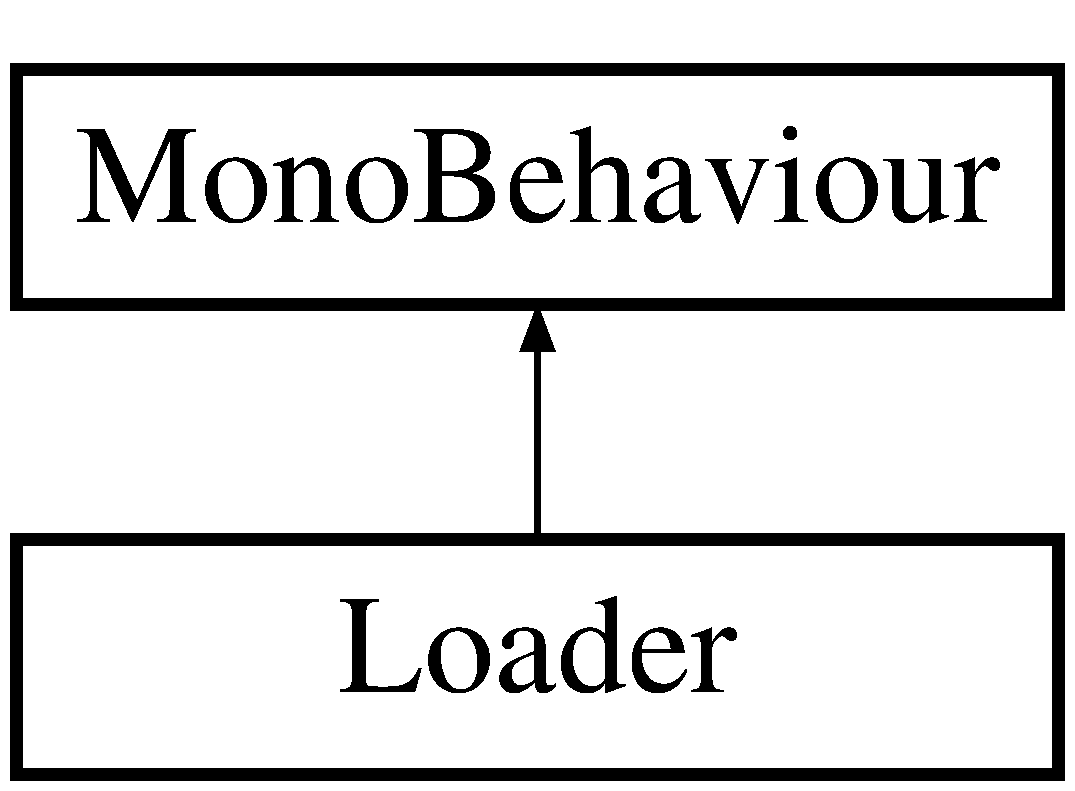
\includegraphics[height=2.000000cm]{class_loader}
\end{center}
\end{figure}
\subsection*{Public Attributes}
\begin{DoxyCompactItemize}
\item 
\mbox{\Hypertarget{class_loader_a4eee44244b0fa6a5708e2ffbee772403}\label{class_loader_a4eee44244b0fa6a5708e2ffbee772403}} 
\mbox{\hyperlink{class_game_manager}{Game\+Manager}} {\bfseries game\+Manager}
\end{DoxyCompactItemize}


The documentation for this class was generated from the following file\+:\begin{DoxyCompactItemize}
\item 
Loader.\+cs\end{DoxyCompactItemize}

\hypertarget{class_main_menu}{}\section{Main\+Menu Class Reference}
\label{class_main_menu}\index{Main\+Menu@{Main\+Menu}}
Inheritance diagram for Main\+Menu\+:\begin{figure}[H]
\begin{center}
\leavevmode
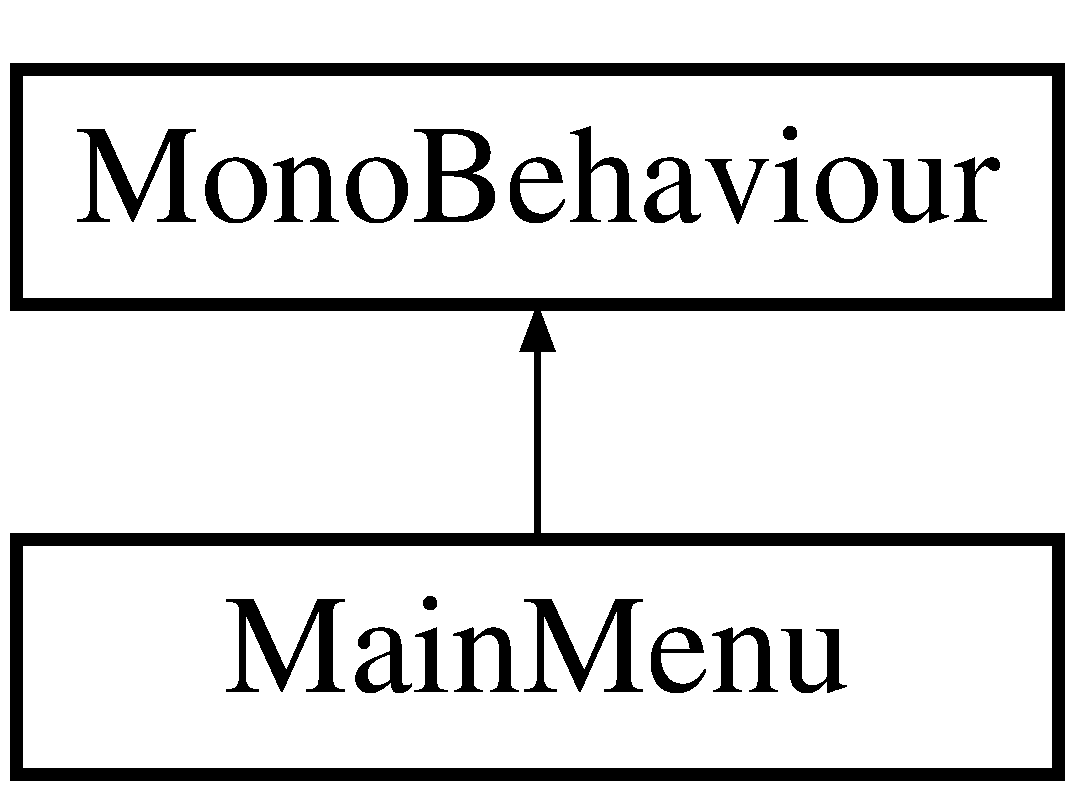
\includegraphics[height=2.000000cm]{class_main_menu}
\end{center}
\end{figure}
\subsection*{Public Member Functions}
\begin{DoxyCompactItemize}
\item 
void \mbox{\hyperlink{class_main_menu_a9a2b50b76ed50c4fc1eb08eba7dc23b2}{Awake}} ()
\item 
void \mbox{\hyperlink{class_main_menu_a11d7e3cd6b90cf59659e03e830e02db5}{Play\+Game}} ()
\item 
void \mbox{\hyperlink{class_main_menu_a485db7cf60c0b93ecc87b9273bcce78b}{Quit\+Game}} ()
\item 
void \mbox{\hyperlink{class_main_menu_a0d0cf4bf03eb9fc4bfcbaef384b6a42e}{Test\+Mode}} ()
\item 
void \mbox{\hyperlink{class_main_menu_a8286e477a22df9031ff4aea9431864ef}{To\+Manual}} ()
\item 
void \mbox{\hyperlink{class_main_menu_ac08c5e57bb188cc5612d644e676245e0}{Back\+Home}} ()
\end{DoxyCompactItemize}
\subsection*{Public Attributes}
\begin{DoxyCompactItemize}
\item 
\mbox{\Hypertarget{class_main_menu_ace51aaeb1e02e402ed09dea424196c4f}\label{class_main_menu_ace51aaeb1e02e402ed09dea424196c4f}} 
Game\+Object {\bfseries manual}
\end{DoxyCompactItemize}


\subsection{Member Function Documentation}
\mbox{\Hypertarget{class_main_menu_a9a2b50b76ed50c4fc1eb08eba7dc23b2}\label{class_main_menu_a9a2b50b76ed50c4fc1eb08eba7dc23b2}} 
\index{Main\+Menu@{Main\+Menu}!Awake@{Awake}}
\index{Awake@{Awake}!Main\+Menu@{Main\+Menu}}
\subsubsection{\texorpdfstring{Awake()}{Awake()}}
{\footnotesize\ttfamily void Main\+Menu.\+Awake (\begin{DoxyParamCaption}{ }\end{DoxyParamCaption})\hspace{0.3cm}{\ttfamily [inline]}}

Awake 
\begin{DoxyParams}{Parameters}
{\em none} & \\
\hline
\end{DoxyParams}
\begin{DoxyReturn}{Returns}
none Opens the main menu 
\end{DoxyReturn}
\mbox{\Hypertarget{class_main_menu_ac08c5e57bb188cc5612d644e676245e0}\label{class_main_menu_ac08c5e57bb188cc5612d644e676245e0}} 
\index{Main\+Menu@{Main\+Menu}!Back\+Home@{Back\+Home}}
\index{Back\+Home@{Back\+Home}!Main\+Menu@{Main\+Menu}}
\subsubsection{\texorpdfstring{Back\+Home()}{BackHome()}}
{\footnotesize\ttfamily void Main\+Menu.\+Back\+Home (\begin{DoxyParamCaption}{ }\end{DoxyParamCaption})\hspace{0.3cm}{\ttfamily [inline]}}

Back\+Home 
\begin{DoxyParams}{Parameters}
{\em none} & \\
\hline
\end{DoxyParams}
\begin{DoxyReturn}{Returns}
none Allows the user to go back to the menu 
\end{DoxyReturn}
\mbox{\Hypertarget{class_main_menu_a11d7e3cd6b90cf59659e03e830e02db5}\label{class_main_menu_a11d7e3cd6b90cf59659e03e830e02db5}} 
\index{Main\+Menu@{Main\+Menu}!Play\+Game@{Play\+Game}}
\index{Play\+Game@{Play\+Game}!Main\+Menu@{Main\+Menu}}
\subsubsection{\texorpdfstring{Play\+Game()}{PlayGame()}}
{\footnotesize\ttfamily void Main\+Menu.\+Play\+Game (\begin{DoxyParamCaption}{ }\end{DoxyParamCaption})\hspace{0.3cm}{\ttfamily [inline]}}

Loads the scene to play the game  None  None \mbox{\Hypertarget{class_main_menu_a485db7cf60c0b93ecc87b9273bcce78b}\label{class_main_menu_a485db7cf60c0b93ecc87b9273bcce78b}} 
\index{Main\+Menu@{Main\+Menu}!Quit\+Game@{Quit\+Game}}
\index{Quit\+Game@{Quit\+Game}!Main\+Menu@{Main\+Menu}}
\subsubsection{\texorpdfstring{Quit\+Game()}{QuitGame()}}
{\footnotesize\ttfamily void Main\+Menu.\+Quit\+Game (\begin{DoxyParamCaption}{ }\end{DoxyParamCaption})\hspace{0.3cm}{\ttfamily [inline]}}

Quits the application  None  None \mbox{\Hypertarget{class_main_menu_a0d0cf4bf03eb9fc4bfcbaef384b6a42e}\label{class_main_menu_a0d0cf4bf03eb9fc4bfcbaef384b6a42e}} 
\index{Main\+Menu@{Main\+Menu}!Test\+Mode@{Test\+Mode}}
\index{Test\+Mode@{Test\+Mode}!Main\+Menu@{Main\+Menu}}
\subsubsection{\texorpdfstring{Test\+Mode()}{TestMode()}}
{\footnotesize\ttfamily void Main\+Menu.\+Test\+Mode (\begin{DoxyParamCaption}{ }\end{DoxyParamCaption})\hspace{0.3cm}{\ttfamily [inline]}}

Test\+Mode 
\begin{DoxyParams}{Parameters}
{\em none} & \\
\hline
\end{DoxyParams}
\begin{DoxyReturn}{Returns}
none Allows the user to go into test mode of the game 
\end{DoxyReturn}
\mbox{\Hypertarget{class_main_menu_a8286e477a22df9031ff4aea9431864ef}\label{class_main_menu_a8286e477a22df9031ff4aea9431864ef}} 
\index{Main\+Menu@{Main\+Menu}!To\+Manual@{To\+Manual}}
\index{To\+Manual@{To\+Manual}!Main\+Menu@{Main\+Menu}}
\subsubsection{\texorpdfstring{To\+Manual()}{ToManual()}}
{\footnotesize\ttfamily void Main\+Menu.\+To\+Manual (\begin{DoxyParamCaption}{ }\end{DoxyParamCaption})\hspace{0.3cm}{\ttfamily [inline]}}

To\+Manual 
\begin{DoxyParams}{Parameters}
{\em none} & \\
\hline
\end{DoxyParams}
\begin{DoxyReturn}{Returns}
none Allows the user to go into the manual 
\end{DoxyReturn}


The documentation for this class was generated from the following file\+:\begin{DoxyCompactItemize}
\item 
Main\+Menu.\+cs\end{DoxyCompactItemize}

\hypertarget{class_map}{}\section{Map Class Reference}
\label{class_map}\index{Map@{Map}}
Inheritance diagram for Map\+:\begin{figure}[H]
\begin{center}
\leavevmode
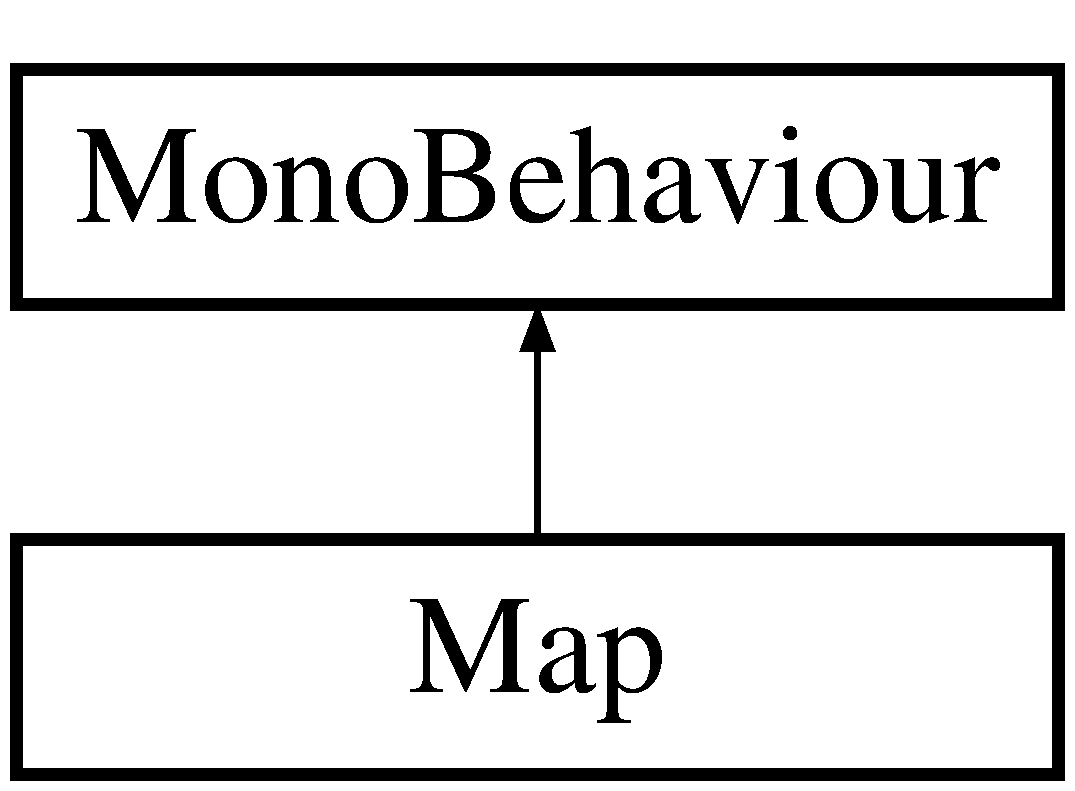
\includegraphics[height=2.000000cm]{class_map}
\end{center}
\end{figure}
\subsection*{Public Member Functions}
\begin{DoxyCompactItemize}
\item 
Transform \mbox{\hyperlink{class_map_a65f298678747e49b6f99ba46271e2519}{Get\+Board\+Holder}} ()
\item 
void \mbox{\hyperlink{class_map_a4b4925269b22d09fc07109d19f8c32e6}{place\+Floors}} ()
\item 
void \mbox{\hyperlink{class_map_a861230d1abdb5ed46e9dc95e8bf61d41}{place\+Walls}} ()
\item 
void \mbox{\hyperlink{class_map_a61d3bb5dbaec40d06efb1b29539f3d2f}{Map\+Setup}} (int cols, int row)
\end{DoxyCompactItemize}
\subsection*{Public Attributes}
\begin{DoxyCompactItemize}
\item 
\mbox{\Hypertarget{class_map_a284e57bb463795f868d0004f2c91ce34}\label{class_map_a284e57bb463795f868d0004f2c91ce34}} 
Game\+Object \mbox{[}$\,$\mbox{]} {\bfseries floor\+Tiles}
\item 
\mbox{\Hypertarget{class_map_abc75d741038130d7b274d5eab51758c1}\label{class_map_abc75d741038130d7b274d5eab51758c1}} 
Game\+Object \mbox{[}$\,$\mbox{]} {\bfseries wall\+Tiles}
\item 
\mbox{\Hypertarget{class_map_a9be8c4808419f525ab5452f1b074c90f}\label{class_map_a9be8c4808419f525ab5452f1b074c90f}} 
List$<$ Vector3 $>$ {\bfseries grid\+Positions} = new List $<$Vector3$>$ ()
\item 
\mbox{\Hypertarget{class_map_a4a5808c38dec273b158a81a6af47e5f5}\label{class_map_a4a5808c38dec273b158a81a6af47e5f5}} 
List$<$ Vector3 $>$ {\bfseries floor\+Positions} = new List $<$Vector3$>$ ()
\item 
\mbox{\Hypertarget{class_map_a86f5dc6f831600a856ee693454bdf308}\label{class_map_a86f5dc6f831600a856ee693454bdf308}} 
int {\bfseries columns}
\item 
\mbox{\Hypertarget{class_map_a4c6ba6b1a6ba20821550e6dd8f8cefbe}\label{class_map_a4c6ba6b1a6ba20821550e6dd8f8cefbe}} 
int {\bfseries rows}
\end{DoxyCompactItemize}


\subsection{Member Function Documentation}
\mbox{\Hypertarget{class_map_a65f298678747e49b6f99ba46271e2519}\label{class_map_a65f298678747e49b6f99ba46271e2519}} 
\index{Map@{Map}!Get\+Board\+Holder@{Get\+Board\+Holder}}
\index{Get\+Board\+Holder@{Get\+Board\+Holder}!Map@{Map}}
\subsubsection{\texorpdfstring{Get\+Board\+Holder()}{GetBoardHolder()}}
{\footnotesize\ttfamily Transform Map.\+Get\+Board\+Holder (\begin{DoxyParamCaption}{ }\end{DoxyParamCaption})\hspace{0.3cm}{\ttfamily [inline]}}

Returns a holder in the hiearchy to hold walls, floor etc...  None  Transform \mbox{\Hypertarget{class_map_a61d3bb5dbaec40d06efb1b29539f3d2f}\label{class_map_a61d3bb5dbaec40d06efb1b29539f3d2f}} 
\index{Map@{Map}!Map\+Setup@{Map\+Setup}}
\index{Map\+Setup@{Map\+Setup}!Map@{Map}}
\subsubsection{\texorpdfstring{Map\+Setup()}{MapSetup()}}
{\footnotesize\ttfamily void Map.\+Map\+Setup (\begin{DoxyParamCaption}\item[{int}]{cols,  }\item[{int}]{row }\end{DoxyParamCaption})\hspace{0.3cm}{\ttfamily [inline]}}

sets the size of the map and calls Board\+Setup()  int cols  int row  None \mbox{\Hypertarget{class_map_a4b4925269b22d09fc07109d19f8c32e6}\label{class_map_a4b4925269b22d09fc07109d19f8c32e6}} 
\index{Map@{Map}!place\+Floors@{place\+Floors}}
\index{place\+Floors@{place\+Floors}!Map@{Map}}
\subsubsection{\texorpdfstring{place\+Floors()}{placeFloors()}}
{\footnotesize\ttfamily void Map.\+place\+Floors (\begin{DoxyParamCaption}{ }\end{DoxyParamCaption})\hspace{0.3cm}{\ttfamily [inline]}}

Place the foor tiles  None  None \mbox{\Hypertarget{class_map_a861230d1abdb5ed46e9dc95e8bf61d41}\label{class_map_a861230d1abdb5ed46e9dc95e8bf61d41}} 
\index{Map@{Map}!place\+Walls@{place\+Walls}}
\index{place\+Walls@{place\+Walls}!Map@{Map}}
\subsubsection{\texorpdfstring{place\+Walls()}{placeWalls()}}
{\footnotesize\ttfamily void Map.\+place\+Walls (\begin{DoxyParamCaption}{ }\end{DoxyParamCaption})\hspace{0.3cm}{\ttfamily [inline]}}

Place the wall tiles  None  None 

The documentation for this class was generated from the following file\+:\begin{DoxyCompactItemize}
\item 
Map.\+cs\end{DoxyCompactItemize}

\hypertarget{class_menu_music}{}\section{Menu\+Music Class Reference}
\label{class_menu_music}\index{Menu\+Music@{Menu\+Music}}
Inheritance diagram for Menu\+Music\+:\begin{figure}[H]
\begin{center}
\leavevmode
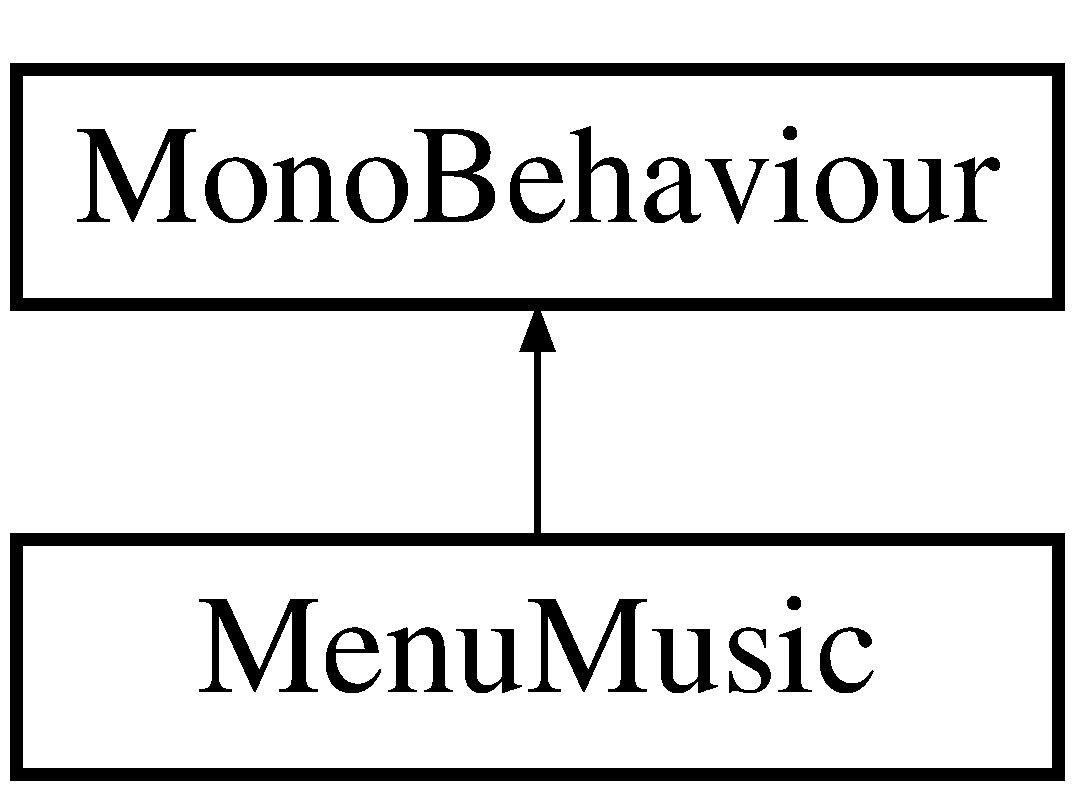
\includegraphics[height=2.000000cm]{class_menu_music}
\end{center}
\end{figure}
\subsection*{Public Member Functions}
\begin{DoxyCompactItemize}
\item 
void \mbox{\hyperlink{class_menu_music_a821a3c7653b3dfee1e1fdf174857109d}{Awake}} ()
\end{DoxyCompactItemize}


\subsection{Member Function Documentation}
\mbox{\Hypertarget{class_menu_music_a821a3c7653b3dfee1e1fdf174857109d}\label{class_menu_music_a821a3c7653b3dfee1e1fdf174857109d}} 
\index{Menu\+Music@{Menu\+Music}!Awake@{Awake}}
\index{Awake@{Awake}!Menu\+Music@{Menu\+Music}}
\subsubsection{\texorpdfstring{Awake()}{Awake()}}
{\footnotesize\ttfamily void Menu\+Music.\+Awake (\begin{DoxyParamCaption}{ }\end{DoxyParamCaption})\hspace{0.3cm}{\ttfamily [inline]}}

Awake 
\begin{DoxyParams}{Parameters}
{\em none} & \\
\hline
\end{DoxyParams}
\begin{DoxyReturn}{Returns}
none Allows only one instance of menu music to play 
\end{DoxyReturn}


The documentation for this class was generated from the following file\+:\begin{DoxyCompactItemize}
\item 
Menu\+Music.\+cs\end{DoxyCompactItemize}

\hypertarget{class_moving_object}{}\section{Moving\+Object Class Reference}
\label{class_moving_object}\index{Moving\+Object@{Moving\+Object}}
Inheritance diagram for Moving\+Object\+:\begin{figure}[H]
\begin{center}
\leavevmode
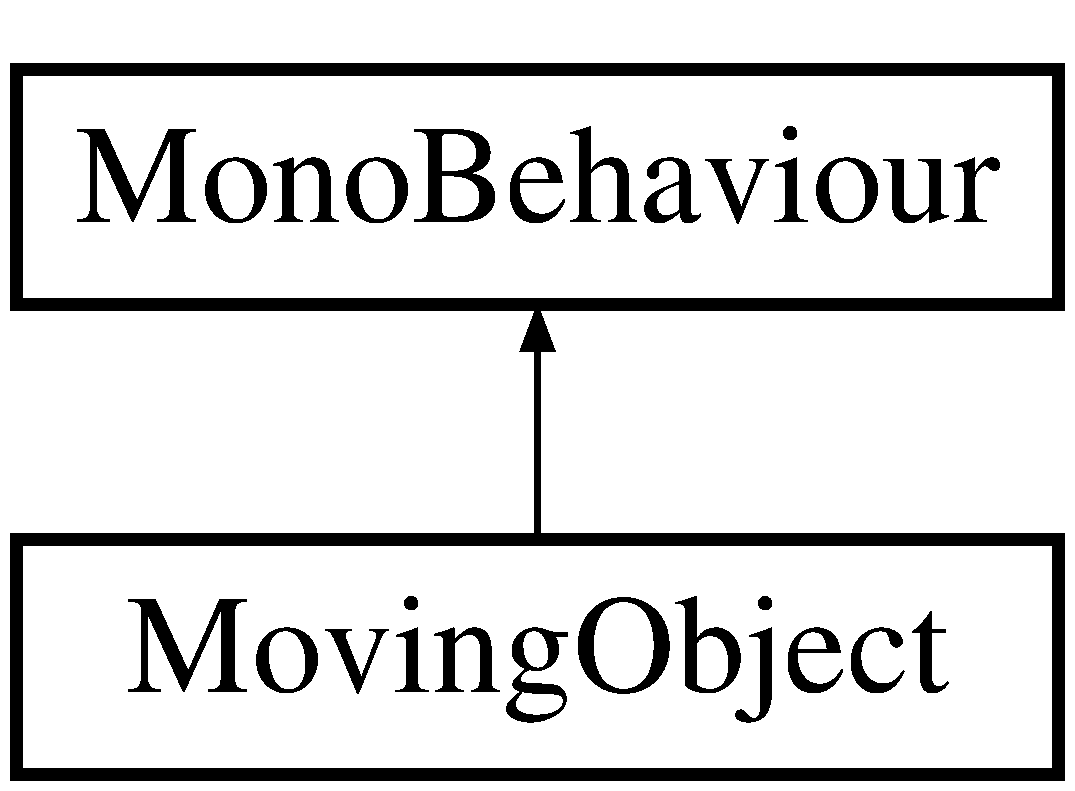
\includegraphics[height=2.000000cm]{class_moving_object}
\end{center}
\end{figure}
\subsection*{Public Attributes}
\begin{DoxyCompactItemize}
\item 
\mbox{\Hypertarget{class_moving_object_a2596eb0312a148176541ac08fb18b173}\label{class_moving_object_a2596eb0312a148176541ac08fb18b173}} 
float {\bfseries move\+Time} = 0.\+1f
\item 
\mbox{\Hypertarget{class_moving_object_add4cf20e336559d38cc6a57763775e36}\label{class_moving_object_add4cf20e336559d38cc6a57763775e36}} 
Layer\+Mask {\bfseries blocking\+Layer}
\end{DoxyCompactItemize}
\subsection*{Protected Member Functions}
\begin{DoxyCompactItemize}
\item 
\mbox{\Hypertarget{class_moving_object_a2b6026a8e7e4313764cb876fd99ae1cd}\label{class_moving_object_a2b6026a8e7e4313764cb876fd99ae1cd}} 
virtual void {\bfseries Start} ()
\item 
\mbox{\Hypertarget{class_moving_object_a3d8df930ae96d375fc1863b483e1c2e5}\label{class_moving_object_a3d8df930ae96d375fc1863b483e1c2e5}} 
bool {\bfseries Move} (float x\+Dir, float y\+Dir, out Raycast\+Hit2D hit)
\item 
\mbox{\Hypertarget{class_moving_object_ab5b0553c2da577c976c7f1416ff6605a}\label{class_moving_object_ab5b0553c2da577c976c7f1416ff6605a}} 
I\+Enumerator {\bfseries Smooth\+Movement} (Vector3 end)
\item 
\mbox{\Hypertarget{class_moving_object_a9cb5a5729151a4f9745a24988176f620}\label{class_moving_object_a9cb5a5729151a4f9745a24988176f620}} 
virtual void {\bfseries Attempt\+Move$<$ T $>$} (float x\+Dir, float y\+Dir)
\item 
\mbox{\Hypertarget{class_moving_object_af20de314364d109abfad1fe0f15d4732}\label{class_moving_object_af20de314364d109abfad1fe0f15d4732}} 
abstract void {\bfseries On\+Cant\+Move$<$ T $>$} (T component)
\end{DoxyCompactItemize}


The documentation for this class was generated from the following file\+:\begin{DoxyCompactItemize}
\item 
Moving\+Object.\+cs\end{DoxyCompactItemize}

\hypertarget{class_muffin_man}{}\section{Muffin\+Man Class Reference}
\label{class_muffin_man}\index{Muffin\+Man@{Muffin\+Man}}
Inheritance diagram for Muffin\+Man\+:\begin{figure}[H]
\begin{center}
\leavevmode
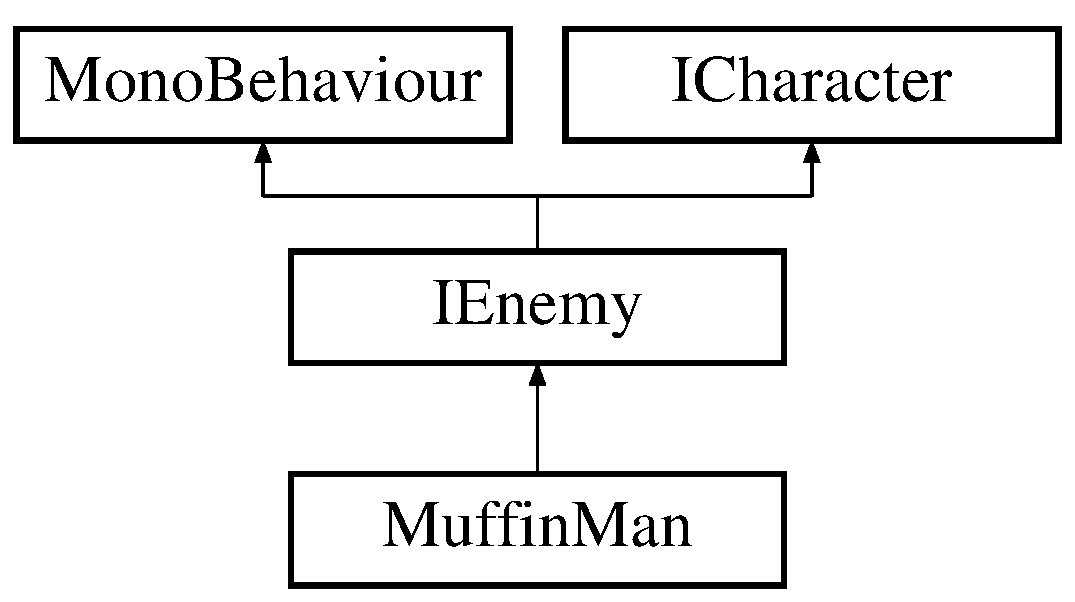
\includegraphics[height=3.000000cm]{class_muffin_man}
\end{center}
\end{figure}
\subsection*{Public Member Functions}
\begin{DoxyCompactItemize}
\item 
void \mbox{\hyperlink{class_muffin_man_aa693b638b6e52ab4fed01d7113b58ca8}{Set\+Move}} (bool value)
\item 
void \mbox{\hyperlink{class_muffin_man_a4b71be125a1beefd38dffd5a35ac8526}{Fixed\+Update}} ()
\item 
void \mbox{\hyperlink{class_muffin_man_a0285a9daaa9c7285ad76570a2166733d}{Take\+Damage}} (int damage\+Taken)
\item 
void \mbox{\hyperlink{class_muffin_man_af917e1ad1d45ee23bd6b7edc5d14e0c5}{Attack}} ()
\item 
void \mbox{\hyperlink{class_muffin_man_ad8d6f582c58fed8b43fd4a7c66ce2411}{set\+Speed}} (int speed)
\item 
void \mbox{\hyperlink{class_muffin_man_a4990952946d39102b3034ee93f70f20d}{set\+Health}} (int health)
\item 
bool \mbox{\hyperlink{class_muffin_man_a0b2cb2eb97c7452da51f40af91c7b4b3}{is\+Dead}} ()
\end{DoxyCompactItemize}
\subsection*{Public Attributes}
\begin{DoxyCompactItemize}
\item 
\mbox{\Hypertarget{class_muffin_man_affaf77ed95a8093c406a308399de06a1}\label{class_muffin_man_affaf77ed95a8093c406a308399de06a1}} 
Vector3 {\bfseries current}
\item 
\mbox{\Hypertarget{class_muffin_man_aafcb38688b56768770d0610ce055c165}\label{class_muffin_man_aafcb38688b56768770d0610ce055c165}} 
Vector3 {\bfseries target}
\end{DoxyCompactItemize}


\subsection{Member Function Documentation}
\mbox{\Hypertarget{class_muffin_man_af917e1ad1d45ee23bd6b7edc5d14e0c5}\label{class_muffin_man_af917e1ad1d45ee23bd6b7edc5d14e0c5}} 
\index{Muffin\+Man@{Muffin\+Man}!Attack@{Attack}}
\index{Attack@{Attack}!Muffin\+Man@{Muffin\+Man}}
\subsubsection{\texorpdfstring{Attack()}{Attack()}}
{\footnotesize\ttfamily void Muffin\+Man.\+Attack (\begin{DoxyParamCaption}{ }\end{DoxyParamCaption})\hspace{0.3cm}{\ttfamily [inline]}}

Attack 
\begin{DoxyParams}{Parameters}
{\em none} & \\
\hline
\end{DoxyParams}
\begin{DoxyReturn}{Returns}
none Uses attack animation of this character 
\end{DoxyReturn}
Attack Left ////

Attack Up ////

Attack Down //// 

Implements \mbox{\hyperlink{interface_i_character}{I\+Character}}.

\mbox{\Hypertarget{class_muffin_man_a4b71be125a1beefd38dffd5a35ac8526}\label{class_muffin_man_a4b71be125a1beefd38dffd5a35ac8526}} 
\index{Muffin\+Man@{Muffin\+Man}!Fixed\+Update@{Fixed\+Update}}
\index{Fixed\+Update@{Fixed\+Update}!Muffin\+Man@{Muffin\+Man}}
\subsubsection{\texorpdfstring{Fixed\+Update()}{FixedUpdate()}}
{\footnotesize\ttfamily void Muffin\+Man.\+Fixed\+Update (\begin{DoxyParamCaption}{ }\end{DoxyParamCaption})\hspace{0.3cm}{\ttfamily [inline]}}

Fixed\+Update 
\begin{DoxyParams}{Parameters}
{\em none} & \\
\hline
\end{DoxyParams}
\begin{DoxyReturn}{Returns}
none Called every .02s 
\end{DoxyReturn}
\mbox{\Hypertarget{class_muffin_man_a0b2cb2eb97c7452da51f40af91c7b4b3}\label{class_muffin_man_a0b2cb2eb97c7452da51f40af91c7b4b3}} 
\index{Muffin\+Man@{Muffin\+Man}!is\+Dead@{is\+Dead}}
\index{is\+Dead@{is\+Dead}!Muffin\+Man@{Muffin\+Man}}
\subsubsection{\texorpdfstring{is\+Dead()}{isDead()}}
{\footnotesize\ttfamily bool Muffin\+Man.\+is\+Dead (\begin{DoxyParamCaption}{ }\end{DoxyParamCaption})\hspace{0.3cm}{\ttfamily [inline]}}

is\+Dead 
\begin{DoxyParams}{Parameters}
{\em none} & \\
\hline
\end{DoxyParams}
\begin{DoxyReturn}{Returns}
bool void 
\end{DoxyReturn}


Implements \mbox{\hyperlink{interface_i_character}{I\+Character}}.

\mbox{\Hypertarget{class_muffin_man_a4990952946d39102b3034ee93f70f20d}\label{class_muffin_man_a4990952946d39102b3034ee93f70f20d}} 
\index{Muffin\+Man@{Muffin\+Man}!set\+Health@{set\+Health}}
\index{set\+Health@{set\+Health}!Muffin\+Man@{Muffin\+Man}}
\subsubsection{\texorpdfstring{set\+Health()}{setHealth()}}
{\footnotesize\ttfamily void Muffin\+Man.\+set\+Health (\begin{DoxyParamCaption}\item[{int}]{health }\end{DoxyParamCaption})\hspace{0.3cm}{\ttfamily [inline]}}

set\+Health 
\begin{DoxyParams}{Parameters}
{\em int} & \\
\hline
\end{DoxyParams}
\begin{DoxyReturn}{Returns}
none void 
\end{DoxyReturn}


Implements \mbox{\hyperlink{interface_i_character}{I\+Character}}.

\mbox{\Hypertarget{class_muffin_man_aa693b638b6e52ab4fed01d7113b58ca8}\label{class_muffin_man_aa693b638b6e52ab4fed01d7113b58ca8}} 
\index{Muffin\+Man@{Muffin\+Man}!Set\+Move@{Set\+Move}}
\index{Set\+Move@{Set\+Move}!Muffin\+Man@{Muffin\+Man}}
\subsubsection{\texorpdfstring{Set\+Move()}{SetMove()}}
{\footnotesize\ttfamily void Muffin\+Man.\+Set\+Move (\begin{DoxyParamCaption}\item[{bool}]{value }\end{DoxyParamCaption})\hspace{0.3cm}{\ttfamily [inline]}}

Set\+Move 
\begin{DoxyParams}{Parameters}
{\em bool} & \\
\hline
\end{DoxyParams}
\begin{DoxyReturn}{Returns}
none sets value of let\+Move 
\end{DoxyReturn}
\mbox{\Hypertarget{class_muffin_man_ad8d6f582c58fed8b43fd4a7c66ce2411}\label{class_muffin_man_ad8d6f582c58fed8b43fd4a7c66ce2411}} 
\index{Muffin\+Man@{Muffin\+Man}!set\+Speed@{set\+Speed}}
\index{set\+Speed@{set\+Speed}!Muffin\+Man@{Muffin\+Man}}
\subsubsection{\texorpdfstring{set\+Speed()}{setSpeed()}}
{\footnotesize\ttfamily void Muffin\+Man.\+set\+Speed (\begin{DoxyParamCaption}\item[{int}]{speed }\end{DoxyParamCaption})\hspace{0.3cm}{\ttfamily [inline]}}

set\+Speed 
\begin{DoxyParams}{Parameters}
{\em int} & \\
\hline
\end{DoxyParams}
\begin{DoxyReturn}{Returns}
none void 
\end{DoxyReturn}


Implements \mbox{\hyperlink{interface_i_character}{I\+Character}}.

\mbox{\Hypertarget{class_muffin_man_a0285a9daaa9c7285ad76570a2166733d}\label{class_muffin_man_a0285a9daaa9c7285ad76570a2166733d}} 
\index{Muffin\+Man@{Muffin\+Man}!Take\+Damage@{Take\+Damage}}
\index{Take\+Damage@{Take\+Damage}!Muffin\+Man@{Muffin\+Man}}
\subsubsection{\texorpdfstring{Take\+Damage()}{TakeDamage()}}
{\footnotesize\ttfamily void Muffin\+Man.\+Take\+Damage (\begin{DoxyParamCaption}\item[{int}]{damage\+Taken }\end{DoxyParamCaption})\hspace{0.3cm}{\ttfamily [inline]}}

Take\+Damage 
\begin{DoxyParams}{Parameters}
{\em int} & \\
\hline
\end{DoxyParams}
\begin{DoxyReturn}{Returns}
none Reduces health of character 
\end{DoxyReturn}


Implements \mbox{\hyperlink{interface_i_character}{I\+Character}}.



The documentation for this class was generated from the following file\+:\begin{DoxyCompactItemize}
\item 
Muffin\+Man.\+cs\end{DoxyCompactItemize}

\hypertarget{class_muffin_man_controller}{}\section{Muffin\+Man\+Controller Class Reference}
\label{class_muffin_man_controller}\index{Muffin\+Man\+Controller@{Muffin\+Man\+Controller}}
Inheritance diagram for Muffin\+Man\+Controller\+:\begin{figure}[H]
\begin{center}
\leavevmode
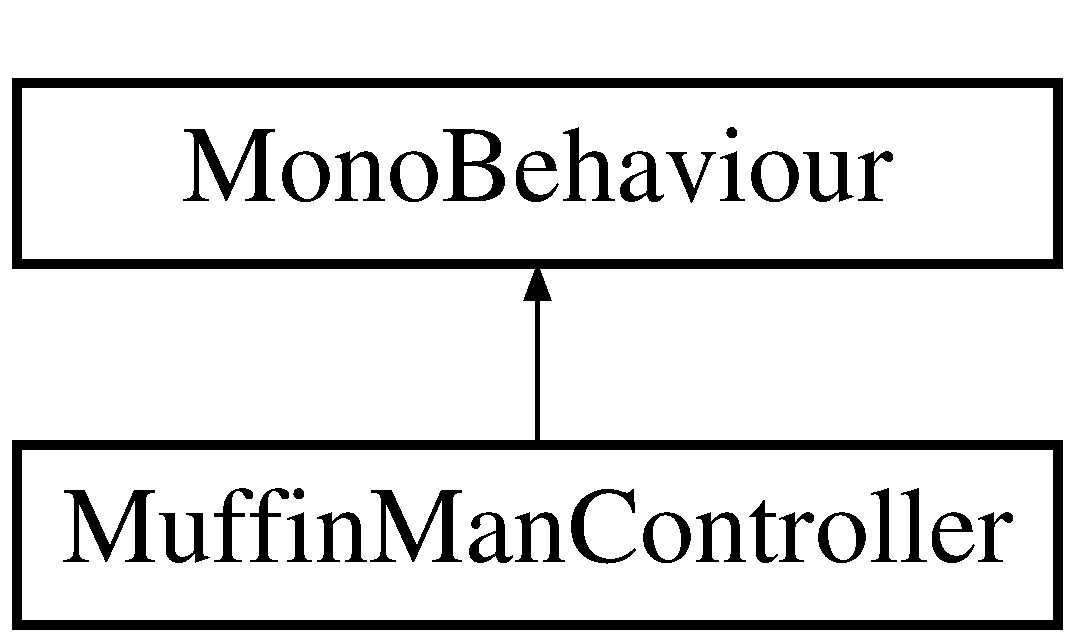
\includegraphics[height=2.000000cm]{class_muffin_man_controller}
\end{center}
\end{figure}
\subsection*{Public Attributes}
\begin{DoxyCompactItemize}
\item 
\mbox{\Hypertarget{class_muffin_man_controller_af5afb2b3cd19f7628413bc563b078bf7}\label{class_muffin_man_controller_af5afb2b3cd19f7628413bc563b078bf7}} 
float {\bfseries speed} = 5.\+0f
\end{DoxyCompactItemize}


The documentation for this class was generated from the following file\+:\begin{DoxyCompactItemize}
\item 
Muffin\+Man\+Controller.\+cs\end{DoxyCompactItemize}

\hypertarget{class_muffin_man_spawner}{}\section{Muffin\+Man\+Spawner Class Reference}
\label{class_muffin_man_spawner}\index{Muffin\+Man\+Spawner@{Muffin\+Man\+Spawner}}
Inheritance diagram for Muffin\+Man\+Spawner\+:\begin{figure}[H]
\begin{center}
\leavevmode
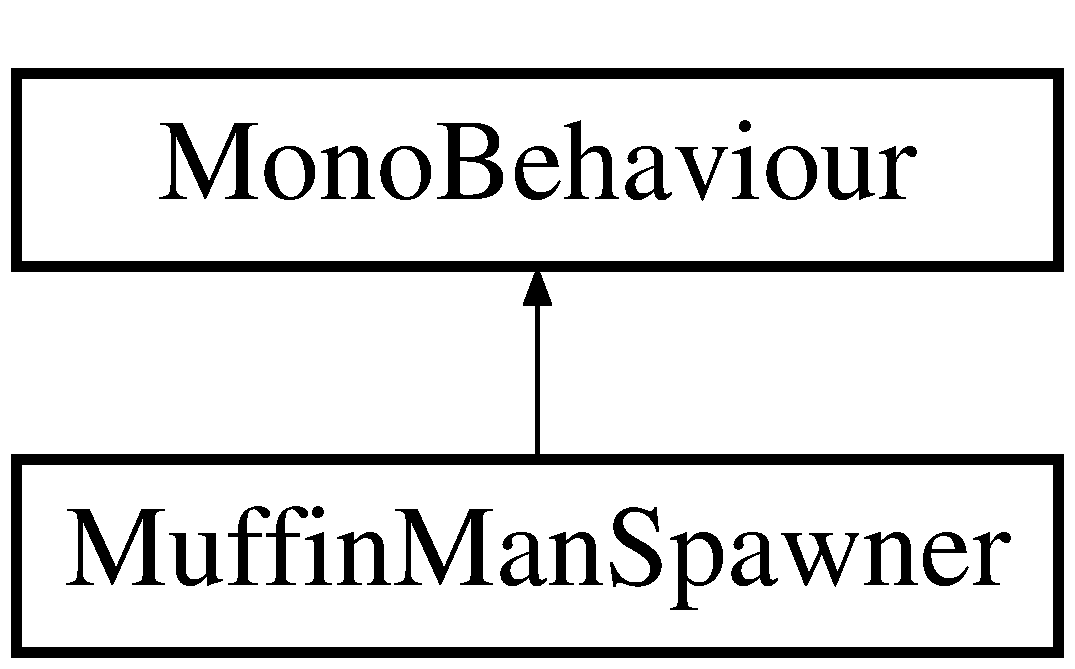
\includegraphics[height=2.000000cm]{class_muffin_man_spawner}
\end{center}
\end{figure}
\subsection*{Public Attributes}
\begin{DoxyCompactItemize}
\item 
\mbox{\Hypertarget{class_muffin_man_spawner_a0defd165e01bdccf49940226a98f1985}\label{class_muffin_man_spawner_a0defd165e01bdccf49940226a98f1985}} 
Game\+Object {\bfseries muffin\+Man}
\end{DoxyCompactItemize}


The documentation for this class was generated from the following file\+:\begin{DoxyCompactItemize}
\item 
Muffin\+Man\+Spawner.\+cs\end{DoxyCompactItemize}

\hypertarget{class_pause_menu}{}\section{Pause\+Menu Class Reference}
\label{class_pause_menu}\index{Pause\+Menu@{Pause\+Menu}}
Inheritance diagram for Pause\+Menu\+:\begin{figure}[H]
\begin{center}
\leavevmode
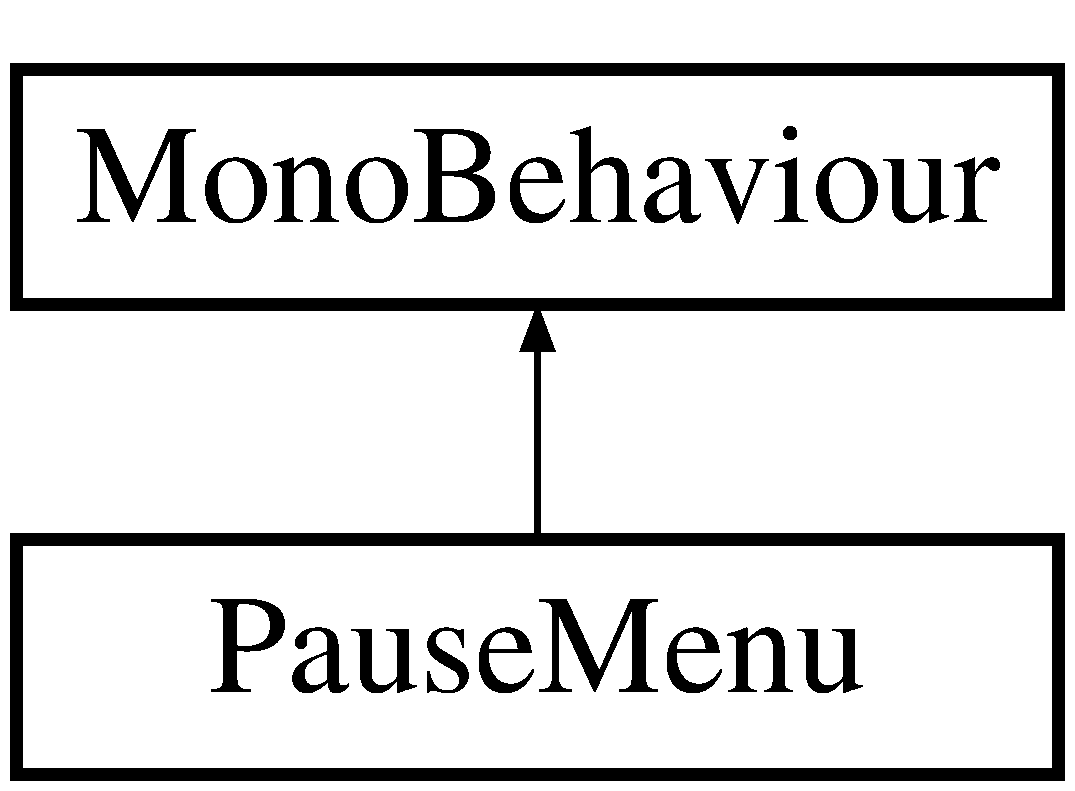
\includegraphics[height=2.000000cm]{class_pause_menu}
\end{center}
\end{figure}
\subsection*{Public Member Functions}
\begin{DoxyCompactItemize}
\item 
void \mbox{\hyperlink{class_pause_menu_a4416b25e65dfadf57cd8657eaf94f7df}{Resume}} ()
\item 
void \mbox{\hyperlink{class_pause_menu_a712dac1268693262de144337e2835ea7}{Pause}} ()
\item 
void \mbox{\hyperlink{class_pause_menu_ad9f370d76d1af2ebdda21eaae4ea5477}{Menu}} ()
\end{DoxyCompactItemize}
\subsection*{Public Attributes}
\begin{DoxyCompactItemize}
\item 
\mbox{\Hypertarget{class_pause_menu_a49305f37ccebc2342ea009f5cb259fee}\label{class_pause_menu_a49305f37ccebc2342ea009f5cb259fee}} 
Game\+Object {\bfseries pause\+Menu\+UI}
\item 
\mbox{\Hypertarget{class_pause_menu_a4a7e503a0ef57ced8f5f732a93c7c6cb}\label{class_pause_menu_a4a7e503a0ef57ced8f5f732a93c7c6cb}} 
Button {\bfseries Pause\+Button}
\end{DoxyCompactItemize}
\subsection*{Static Public Attributes}
\begin{DoxyCompactItemize}
\item 
\mbox{\Hypertarget{class_pause_menu_a4ca5f2ef5197fa89f9ecb4d6d4f47560}\label{class_pause_menu_a4ca5f2ef5197fa89f9ecb4d6d4f47560}} 
static bool {\bfseries Game\+Is\+Paused} = false
\end{DoxyCompactItemize}


\subsection{Member Function Documentation}
\mbox{\Hypertarget{class_pause_menu_ad9f370d76d1af2ebdda21eaae4ea5477}\label{class_pause_menu_ad9f370d76d1af2ebdda21eaae4ea5477}} 
\index{Pause\+Menu@{Pause\+Menu}!Menu@{Menu}}
\index{Menu@{Menu}!Pause\+Menu@{Pause\+Menu}}
\subsubsection{\texorpdfstring{Menu()}{Menu()}}
{\footnotesize\ttfamily void Pause\+Menu.\+Menu (\begin{DoxyParamCaption}{ }\end{DoxyParamCaption})\hspace{0.3cm}{\ttfamily [inline]}}

Makes sure to resume time when the main menu option is selected  None  None \mbox{\Hypertarget{class_pause_menu_a712dac1268693262de144337e2835ea7}\label{class_pause_menu_a712dac1268693262de144337e2835ea7}} 
\index{Pause\+Menu@{Pause\+Menu}!Pause@{Pause}}
\index{Pause@{Pause}!Pause\+Menu@{Pause\+Menu}}
\subsubsection{\texorpdfstring{Pause()}{Pause()}}
{\footnotesize\ttfamily void Pause\+Menu.\+Pause (\begin{DoxyParamCaption}{ }\end{DoxyParamCaption})\hspace{0.3cm}{\ttfamily [inline]}}

Pauses time in-\/game  None  None \mbox{\Hypertarget{class_pause_menu_a4416b25e65dfadf57cd8657eaf94f7df}\label{class_pause_menu_a4416b25e65dfadf57cd8657eaf94f7df}} 
\index{Pause\+Menu@{Pause\+Menu}!Resume@{Resume}}
\index{Resume@{Resume}!Pause\+Menu@{Pause\+Menu}}
\subsubsection{\texorpdfstring{Resume()}{Resume()}}
{\footnotesize\ttfamily void Pause\+Menu.\+Resume (\begin{DoxyParamCaption}{ }\end{DoxyParamCaption})\hspace{0.3cm}{\ttfamily [inline]}}

Resumes time in-\/game  None  None 

The documentation for this class was generated from the following file\+:\begin{DoxyCompactItemize}
\item 
Pause\+Menu.\+cs\end{DoxyCompactItemize}

\hypertarget{class_player1_controller}{}\section{Player1\+Controller Class Reference}
\label{class_player1_controller}\index{Player1\+Controller@{Player1\+Controller}}
Inheritance diagram for Player1\+Controller\+:\begin{figure}[H]
\begin{center}
\leavevmode
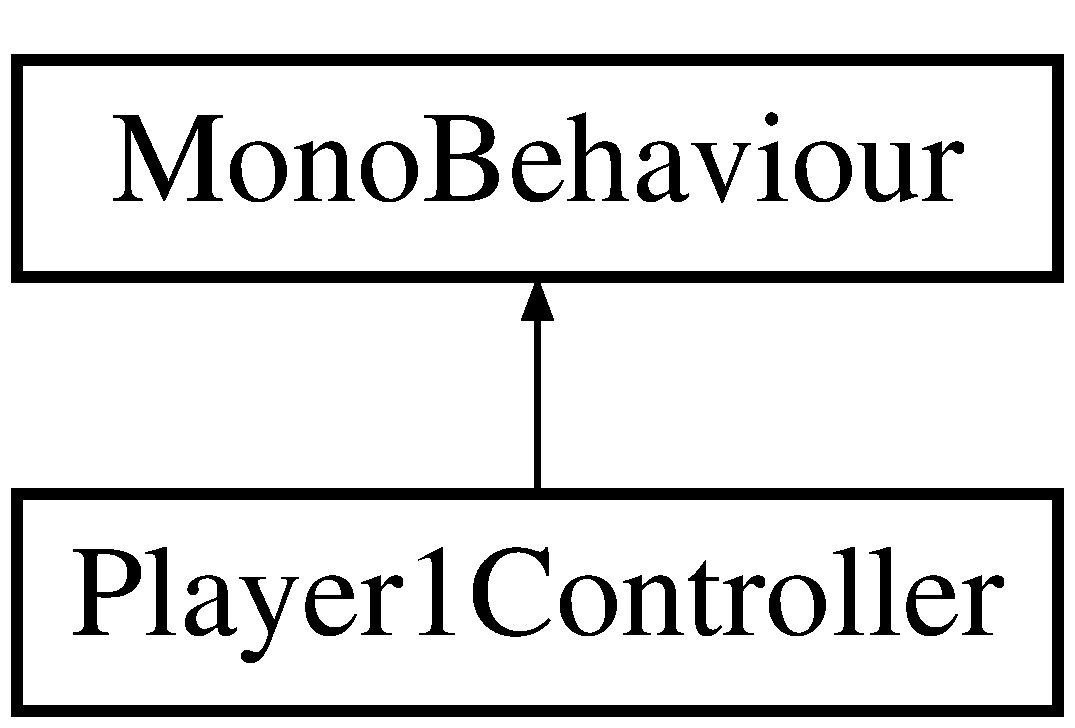
\includegraphics[height=2.000000cm]{class_player1_controller}
\end{center}
\end{figure}
\subsection*{Public Attributes}
\begin{DoxyCompactItemize}
\item 
\mbox{\Hypertarget{class_player1_controller_aa55159a8266e6963c928b73619aae4e9}\label{class_player1_controller_aa55159a8266e6963c928b73619aae4e9}} 
float {\bfseries speed} = 5.\+0f
\item 
\mbox{\Hypertarget{class_player1_controller_a8042e7200e7edf15cf8f64fd8015f04e}\label{class_player1_controller_a8042e7200e7edf15cf8f64fd8015f04e}} 
Game\+Object {\bfseries enemy\+Target}
\item 
\mbox{\Hypertarget{class_player1_controller_a8e149507b7d18b70c7533d1135ed6fcd}\label{class_player1_controller_a8e149507b7d18b70c7533d1135ed6fcd}} 
int {\bfseries attack\+Count}
\end{DoxyCompactItemize}


The documentation for this class was generated from the following file\+:\begin{DoxyCompactItemize}
\item 
Player1\+Controller.\+cs\end{DoxyCompactItemize}

\hypertarget{class_player2_controller}{}\section{Player2\+Controller Class Reference}
\label{class_player2_controller}\index{Player2\+Controller@{Player2\+Controller}}
Inheritance diagram for Player2\+Controller\+:\begin{figure}[H]
\begin{center}
\leavevmode
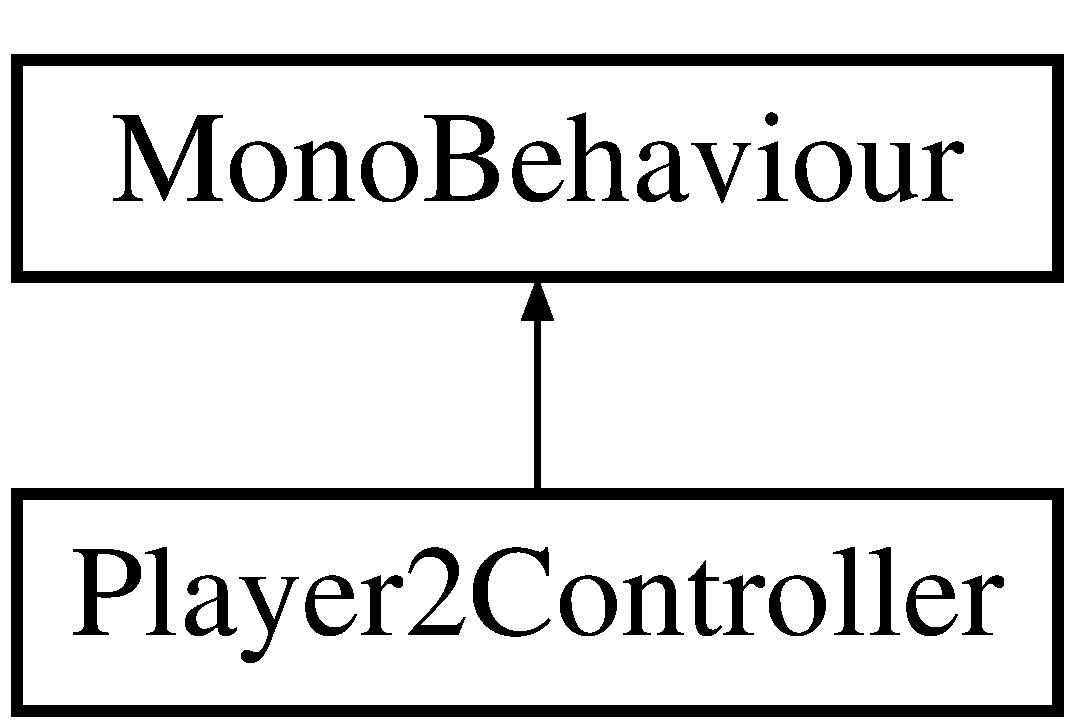
\includegraphics[height=2.000000cm]{class_player2_controller}
\end{center}
\end{figure}
\subsection*{Public Attributes}
\begin{DoxyCompactItemize}
\item 
\mbox{\Hypertarget{class_player2_controller_ac0e96ba11800855ced73543807248d5a}\label{class_player2_controller_ac0e96ba11800855ced73543807248d5a}} 
float {\bfseries speed} = 5.\+0f
\item 
\mbox{\Hypertarget{class_player2_controller_ad9784cd2f1a6d39831884da13208e97e}\label{class_player2_controller_ad9784cd2f1a6d39831884da13208e97e}} 
Game\+Object {\bfseries enemy\+Target}
\item 
\mbox{\Hypertarget{class_player2_controller_abb025e699d97733c6a12ca3680799ca8}\label{class_player2_controller_abb025e699d97733c6a12ca3680799ca8}} 
int {\bfseries attack\+Count}
\end{DoxyCompactItemize}


The documentation for this class was generated from the following file\+:\begin{DoxyCompactItemize}
\item 
Player2\+Controller.\+cs\end{DoxyCompactItemize}

\hypertarget{class_player_selector}{}\section{Player\+Selector Class Reference}
\label{class_player_selector}\index{Player\+Selector@{Player\+Selector}}
Inheritance diagram for Player\+Selector\+:\begin{figure}[H]
\begin{center}
\leavevmode
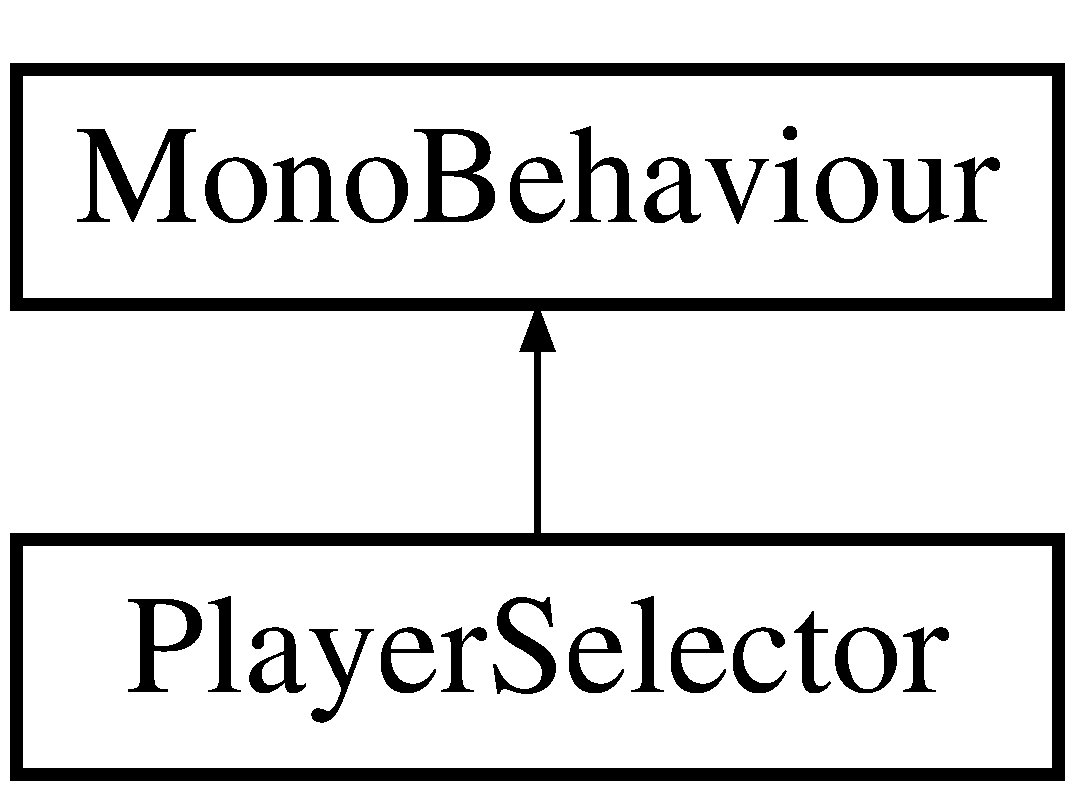
\includegraphics[height=2.000000cm]{class_player_selector}
\end{center}
\end{figure}
\subsection*{Public Member Functions}
\begin{DoxyCompactItemize}
\item 
void \mbox{\hyperlink{class_player_selector_a8114972f187d61d0a9b7e746bf667b1c}{Select\+Gingy}} ()
\item 
void \mbox{\hyperlink{class_player_selector_a310dcc76ad225744be3a0f898c8aea38}{Select\+Shadow\+Gingy}} ()
\end{DoxyCompactItemize}


\subsection{Member Function Documentation}
\mbox{\Hypertarget{class_player_selector_a8114972f187d61d0a9b7e746bf667b1c}\label{class_player_selector_a8114972f187d61d0a9b7e746bf667b1c}} 
\index{Player\+Selector@{Player\+Selector}!Select\+Gingy@{Select\+Gingy}}
\index{Select\+Gingy@{Select\+Gingy}!Player\+Selector@{Player\+Selector}}
\subsubsection{\texorpdfstring{Select\+Gingy()}{SelectGingy()}}
{\footnotesize\ttfamily void Player\+Selector.\+Select\+Gingy (\begin{DoxyParamCaption}{ }\end{DoxyParamCaption})\hspace{0.3cm}{\ttfamily [inline]}}

Select\+Gingy 
\begin{DoxyParams}{Parameters}
{\em none} & \\
\hline
\end{DoxyParams}
\begin{DoxyReturn}{Returns}
none Selects gingy as the player 
\end{DoxyReturn}
\mbox{\Hypertarget{class_player_selector_a310dcc76ad225744be3a0f898c8aea38}\label{class_player_selector_a310dcc76ad225744be3a0f898c8aea38}} 
\index{Player\+Selector@{Player\+Selector}!Select\+Shadow\+Gingy@{Select\+Shadow\+Gingy}}
\index{Select\+Shadow\+Gingy@{Select\+Shadow\+Gingy}!Player\+Selector@{Player\+Selector}}
\subsubsection{\texorpdfstring{Select\+Shadow\+Gingy()}{SelectShadowGingy()}}
{\footnotesize\ttfamily void Player\+Selector.\+Select\+Shadow\+Gingy (\begin{DoxyParamCaption}{ }\end{DoxyParamCaption})\hspace{0.3cm}{\ttfamily [inline]}}

Select\+Shadow\+Gingy 
\begin{DoxyParams}{Parameters}
{\em none} & \\
\hline
\end{DoxyParams}
\begin{DoxyReturn}{Returns}
none Selects Shadow \mbox{\hyperlink{class_gingy}{Gingy}} as the player 
\end{DoxyReturn}


The documentation for this class was generated from the following file\+:\begin{DoxyCompactItemize}
\item 
Player\+Selector.\+cs\end{DoxyCompactItemize}

\hypertarget{class_shadow_gingy}{}\section{Shadow\+Gingy Class Reference}
\label{class_shadow_gingy}\index{Shadow\+Gingy@{Shadow\+Gingy}}
Inheritance diagram for Shadow\+Gingy\+:\begin{figure}[H]
\begin{center}
\leavevmode
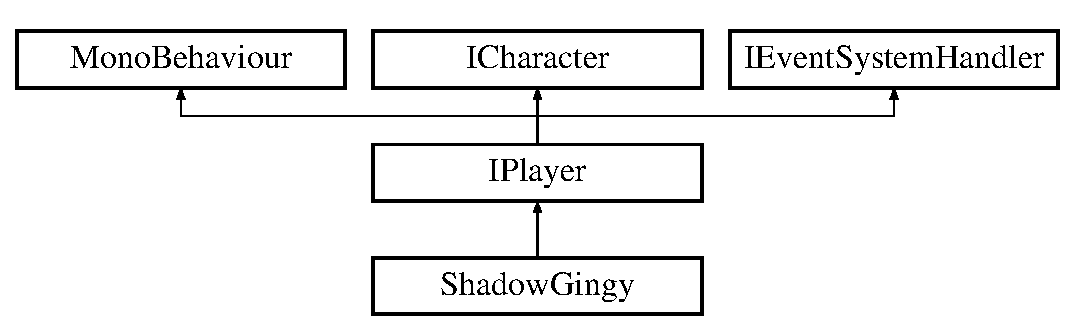
\includegraphics[height=3.000000cm]{class_shadow_gingy}
\end{center}
\end{figure}
\subsection*{Public Member Functions}
\begin{DoxyCompactItemize}
\item 
int \mbox{\hyperlink{class_shadow_gingy_afc294713e7f9a65351df2dd45dade854}{Get\+Health}} ()
\item 
void \mbox{\hyperlink{class_shadow_gingy_a748db29527d960eb1de77379f4586234}{Set\+Health}} (int value)
\end{DoxyCompactItemize}
\subsection*{Additional Inherited Members}


\subsection{Member Function Documentation}
\mbox{\Hypertarget{class_shadow_gingy_afc294713e7f9a65351df2dd45dade854}\label{class_shadow_gingy_afc294713e7f9a65351df2dd45dade854}} 
\index{Shadow\+Gingy@{Shadow\+Gingy}!Get\+Health@{Get\+Health}}
\index{Get\+Health@{Get\+Health}!Shadow\+Gingy@{Shadow\+Gingy}}
\subsubsection{\texorpdfstring{Get\+Health()}{GetHealth()}}
{\footnotesize\ttfamily int Shadow\+Gingy.\+Get\+Health (\begin{DoxyParamCaption}{ }\end{DoxyParamCaption})\hspace{0.3cm}{\ttfamily [inline]}}

Get\+Health 
\begin{DoxyParams}{Parameters}
{\em none} & \\
\hline
\end{DoxyParams}
\begin{DoxyReturn}{Returns}
int returns health 
\end{DoxyReturn}
\mbox{\Hypertarget{class_shadow_gingy_a748db29527d960eb1de77379f4586234}\label{class_shadow_gingy_a748db29527d960eb1de77379f4586234}} 
\index{Shadow\+Gingy@{Shadow\+Gingy}!Set\+Health@{Set\+Health}}
\index{Set\+Health@{Set\+Health}!Shadow\+Gingy@{Shadow\+Gingy}}
\subsubsection{\texorpdfstring{Set\+Health()}{SetHealth()}}
{\footnotesize\ttfamily void Shadow\+Gingy.\+Set\+Health (\begin{DoxyParamCaption}\item[{int}]{value }\end{DoxyParamCaption})\hspace{0.3cm}{\ttfamily [inline]}}

Set\+Health 
\begin{DoxyParams}{Parameters}
{\em int} & \\
\hline
\end{DoxyParams}
\begin{DoxyReturn}{Returns}
none Sets the health 
\end{DoxyReturn}


The documentation for this class was generated from the following file\+:\begin{DoxyCompactItemize}
\item 
Shadow\+Gingy.\+cs\end{DoxyCompactItemize}

\hypertarget{class_test_level}{}\section{Test\+Level Class Reference}
\label{class_test_level}\index{Test\+Level@{Test\+Level}}
Inheritance diagram for Test\+Level\+:\begin{figure}[H]
\begin{center}
\leavevmode
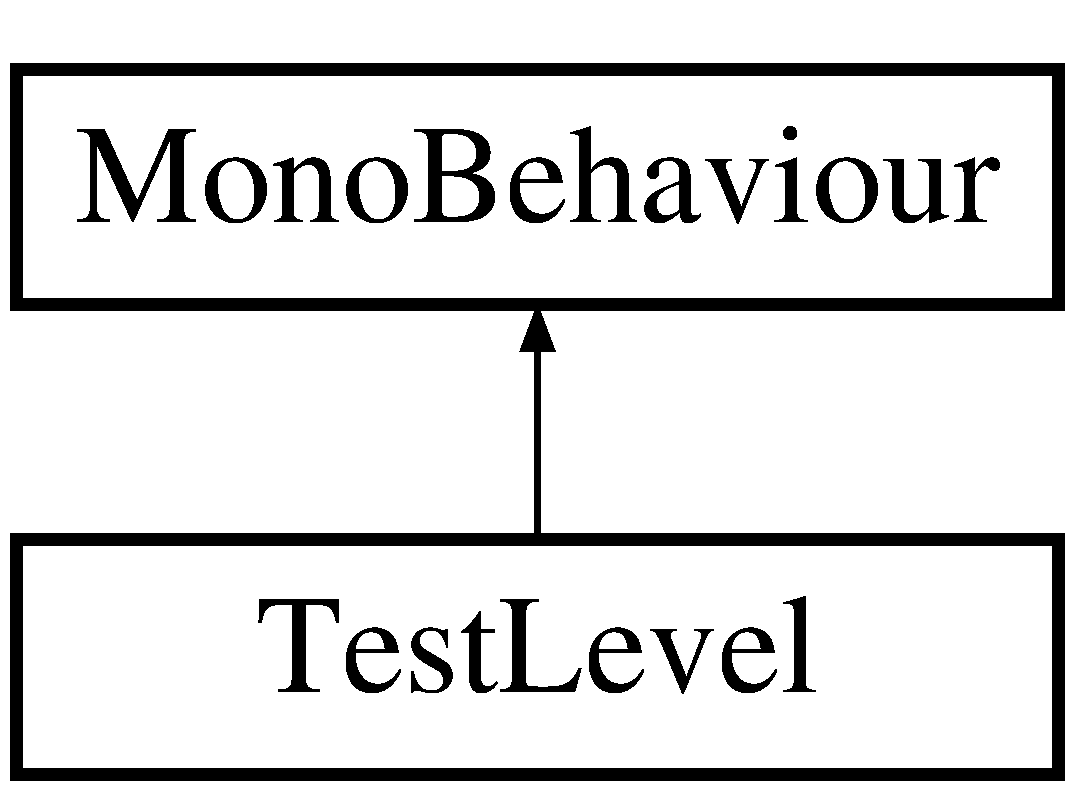
\includegraphics[height=2.000000cm]{class_test_level}
\end{center}
\end{figure}
\subsection*{Public Member Functions}
\begin{DoxyCompactItemize}
\item 
void \mbox{\hyperlink{class_test_level_a6834e350643e7c5bf7ed27d2632f2c92}{Build\+Test\+Level}} ()
\item 
void \mbox{\hyperlink{class_test_level_a7d2ab938df8d29835dee0e7c0defb8e0}{Place\+Player}} (Game\+Object main\+Character)
\item 
void \mbox{\hyperlink{class_test_level_a364cafbd3aa2773d6bba94c313eb0b21}{Place\+Spawners}} ()
\item 
void \mbox{\hyperlink{class_test_level_aaad14a792f3c43f6fb9cb012b1dec89d}{Spawn\+Object}} (Game\+Object obj)
\end{DoxyCompactItemize}
\subsection*{Public Attributes}
\begin{DoxyCompactItemize}
\item 
\mbox{\Hypertarget{class_test_level_a1b517c351d28f2e214f2a4ffcecd98b4}\label{class_test_level_a1b517c351d28f2e214f2a4ffcecd98b4}} 
Game\+Object \mbox{[}$\,$\mbox{]} {\bfseries wall\+Tiles}
\item 
\mbox{\Hypertarget{class_test_level_a1378b22cc8c3128b2de1b933a6f0d574}\label{class_test_level_a1378b22cc8c3128b2de1b933a6f0d574}} 
Game\+Object \mbox{[}$\,$\mbox{]} {\bfseries floor\+Tiles}
\item 
\mbox{\Hypertarget{class_test_level_aed8bd275dd8159fb0fd3e5033244234a}\label{class_test_level_aed8bd275dd8159fb0fd3e5033244234a}} 
Game\+Object {\bfseries muffin\+Man\+Spawner}
\item 
\mbox{\Hypertarget{class_test_level_a17aaa8874ebb24bdf00ccd79ca9fabda}\label{class_test_level_a17aaa8874ebb24bdf00ccd79ca9fabda}} 
Game\+Object {\bfseries jack\+Spawner}
\item 
\mbox{\Hypertarget{class_test_level_af0fc2bc686159feb9dec976899ae7a1a}\label{class_test_level_af0fc2bc686159feb9dec976899ae7a1a}} 
Game\+Object {\bfseries health\+Item\+Spawner}
\item 
\mbox{\Hypertarget{class_test_level_abb2b6d9e0b6f37021873c89de819032c}\label{class_test_level_abb2b6d9e0b6f37021873c89de819032c}} 
Game\+Object {\bfseries invincible\+Item\+Spawner}
\item 
\mbox{\Hypertarget{class_test_level_ad6b394505c2aa79d09340a9ad47ddeb1}\label{class_test_level_ad6b394505c2aa79d09340a9ad47ddeb1}} 
Game\+Object {\bfseries attack\+Item\+Spawner}
\end{DoxyCompactItemize}


\subsection{Member Function Documentation}
\mbox{\Hypertarget{class_test_level_a6834e350643e7c5bf7ed27d2632f2c92}\label{class_test_level_a6834e350643e7c5bf7ed27d2632f2c92}} 
\index{Test\+Level@{Test\+Level}!Build\+Test\+Level@{Build\+Test\+Level}}
\index{Build\+Test\+Level@{Build\+Test\+Level}!Test\+Level@{Test\+Level}}
\subsubsection{\texorpdfstring{Build\+Test\+Level()}{BuildTestLevel()}}
{\footnotesize\ttfamily void Test\+Level.\+Build\+Test\+Level (\begin{DoxyParamCaption}{ }\end{DoxyParamCaption})\hspace{0.3cm}{\ttfamily [inline]}}

Build\+Test\+Level 
\begin{DoxyParams}{Parameters}
{\em none} & \\
\hline
\end{DoxyParams}
\begin{DoxyReturn}{Returns}
none In Charge building and setting up the test level 
\end{DoxyReturn}
\mbox{\Hypertarget{class_test_level_a7d2ab938df8d29835dee0e7c0defb8e0}\label{class_test_level_a7d2ab938df8d29835dee0e7c0defb8e0}} 
\index{Test\+Level@{Test\+Level}!Place\+Player@{Place\+Player}}
\index{Place\+Player@{Place\+Player}!Test\+Level@{Test\+Level}}
\subsubsection{\texorpdfstring{Place\+Player()}{PlacePlayer()}}
{\footnotesize\ttfamily void Test\+Level.\+Place\+Player (\begin{DoxyParamCaption}\item[{Game\+Object}]{main\+Character }\end{DoxyParamCaption})\hspace{0.3cm}{\ttfamily [inline]}}

Place\+Player 
\begin{DoxyParams}{Parameters}
{\em Game\+Object} & main\+Character \\
\hline
\end{DoxyParams}
\begin{DoxyReturn}{Returns}
none Places the main\+Character in the bottom left hand corner 
\end{DoxyReturn}
\mbox{\Hypertarget{class_test_level_a364cafbd3aa2773d6bba94c313eb0b21}\label{class_test_level_a364cafbd3aa2773d6bba94c313eb0b21}} 
\index{Test\+Level@{Test\+Level}!Place\+Spawners@{Place\+Spawners}}
\index{Place\+Spawners@{Place\+Spawners}!Test\+Level@{Test\+Level}}
\subsubsection{\texorpdfstring{Place\+Spawners()}{PlaceSpawners()}}
{\footnotesize\ttfamily void Test\+Level.\+Place\+Spawners (\begin{DoxyParamCaption}{ }\end{DoxyParamCaption})\hspace{0.3cm}{\ttfamily [inline]}}

Place\+Spawners 
\begin{DoxyParams}{Parameters}
{\em none} & \\
\hline
\end{DoxyParams}
\begin{DoxyReturn}{Returns}
none Places the spawners in the central area of the map 
\end{DoxyReturn}
\mbox{\Hypertarget{class_test_level_aaad14a792f3c43f6fb9cb012b1dec89d}\label{class_test_level_aaad14a792f3c43f6fb9cb012b1dec89d}} 
\index{Test\+Level@{Test\+Level}!Spawn\+Object@{Spawn\+Object}}
\index{Spawn\+Object@{Spawn\+Object}!Test\+Level@{Test\+Level}}
\subsubsection{\texorpdfstring{Spawn\+Object()}{SpawnObject()}}
{\footnotesize\ttfamily void Test\+Level.\+Spawn\+Object (\begin{DoxyParamCaption}\item[{Game\+Object}]{obj }\end{DoxyParamCaption})\hspace{0.3cm}{\ttfamily [inline]}}

Spawn\+Object 
\begin{DoxyParams}{Parameters}
{\em Game\+Object} & \\
\hline
\end{DoxyParams}
\begin{DoxyReturn}{Returns}
none Spawns Game\+Object passed in to a random spot in the map 
\end{DoxyReturn}


The documentation for this class was generated from the following file\+:\begin{DoxyCompactItemize}
\item 
Test\+Level.\+cs\end{DoxyCompactItemize}

\hypertarget{class_test_loader}{}\section{Test\+Loader Class Reference}
\label{class_test_loader}\index{Test\+Loader@{Test\+Loader}}
Inheritance diagram for Test\+Loader\+:\begin{figure}[H]
\begin{center}
\leavevmode
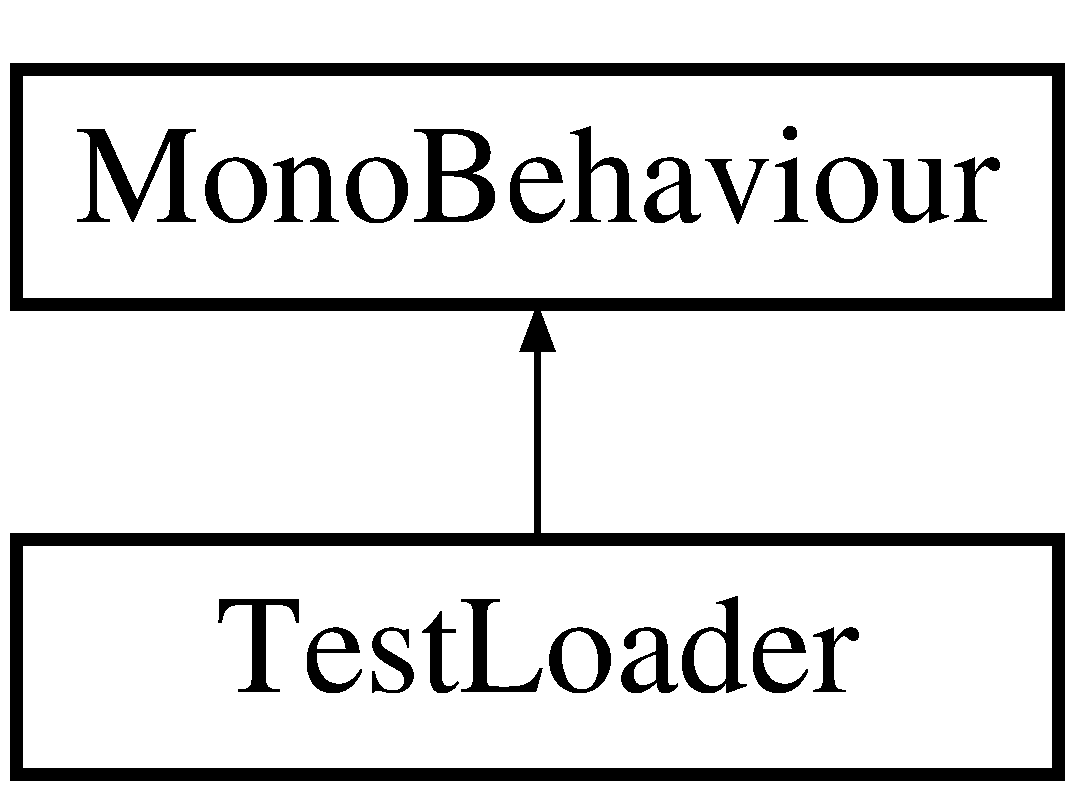
\includegraphics[height=2.000000cm]{class_test_loader}
\end{center}
\end{figure}
\subsection*{Public Attributes}
\begin{DoxyCompactItemize}
\item 
\mbox{\Hypertarget{class_test_loader_a87ab33aa8b5c48dde4f237e280d2fe61}\label{class_test_loader_a87ab33aa8b5c48dde4f237e280d2fe61}} 
\mbox{\hyperlink{class_test_manager}{Test\+Manager}} {\bfseries test\+Manager}
\end{DoxyCompactItemize}


The documentation for this class was generated from the following file\+:\begin{DoxyCompactItemize}
\item 
Test\+Loader.\+cs\end{DoxyCompactItemize}

\hypertarget{class_test_manager}{}\section{Test\+Manager Class Reference}
\label{class_test_manager}\index{Test\+Manager@{Test\+Manager}}
Inheritance diagram for Test\+Manager\+:\begin{figure}[H]
\begin{center}
\leavevmode
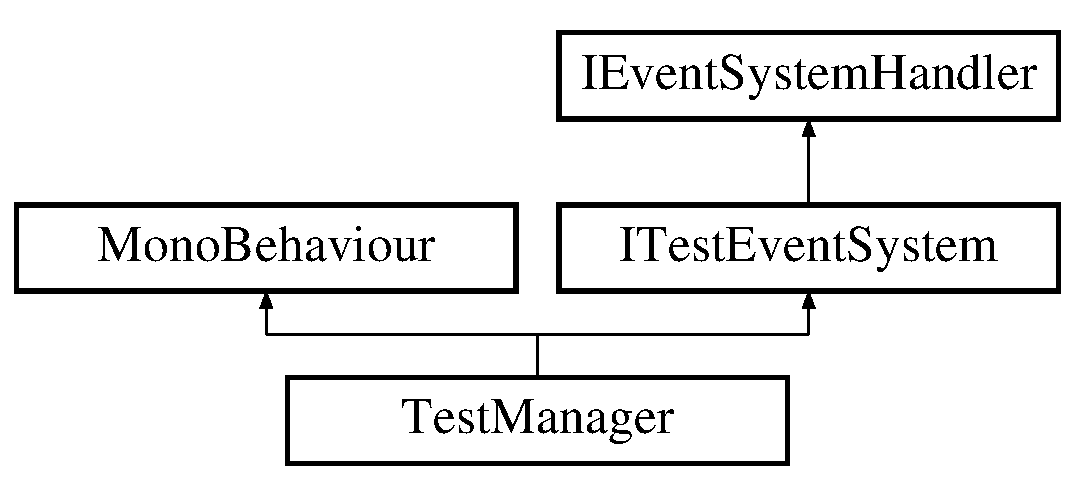
\includegraphics[height=3.000000cm]{class_test_manager}
\end{center}
\end{figure}
\subsection*{Public Member Functions}
\begin{DoxyCompactItemize}
\item 
void \mbox{\hyperlink{class_test_manager_a39a04c0d50c7be1322ad25e67696e549}{End\+Test}} ()
\item 
void \mbox{\hyperlink{class_test_manager_a74fe528d0e18c4cca484bca002dc4f2b}{Start\+Test}} ()
\end{DoxyCompactItemize}
\subsection*{Public Attributes}
\begin{DoxyCompactItemize}
\item 
\mbox{\Hypertarget{class_test_manager_a646d6f59306b6a25f01e8932631141f0}\label{class_test_manager_a646d6f59306b6a25f01e8932631141f0}} 
\mbox{\hyperlink{class_test_level}{Test\+Level}} {\bfseries test\+Level}
\item 
\mbox{\Hypertarget{class_test_manager_ab9a370ea797c52da429e8977799d39cb}\label{class_test_manager_ab9a370ea797c52da429e8977799d39cb}} 
Game\+Object {\bfseries main\+Character}
\end{DoxyCompactItemize}


\subsection{Member Function Documentation}
\mbox{\Hypertarget{class_test_manager_a39a04c0d50c7be1322ad25e67696e549}\label{class_test_manager_a39a04c0d50c7be1322ad25e67696e549}} 
\index{Test\+Manager@{Test\+Manager}!End\+Test@{End\+Test}}
\index{End\+Test@{End\+Test}!Test\+Manager@{Test\+Manager}}
\subsubsection{\texorpdfstring{End\+Test()}{EndTest()}}
{\footnotesize\ttfamily void Test\+Manager.\+End\+Test (\begin{DoxyParamCaption}{ }\end{DoxyParamCaption})\hspace{0.3cm}{\ttfamily [inline]}}

End\+Test 
\begin{DoxyParams}{Parameters}
{\em none} & \\
\hline
\end{DoxyParams}
\begin{DoxyReturn}{Returns}
none Ends the test mode 
\end{DoxyReturn}


Implements \mbox{\hyperlink{interface_i_test_event_system_ae8eda94179d81c4c839a32432216df7b}{I\+Test\+Event\+System}}.

\mbox{\Hypertarget{class_test_manager_a74fe528d0e18c4cca484bca002dc4f2b}\label{class_test_manager_a74fe528d0e18c4cca484bca002dc4f2b}} 
\index{Test\+Manager@{Test\+Manager}!Start\+Test@{Start\+Test}}
\index{Start\+Test@{Start\+Test}!Test\+Manager@{Test\+Manager}}
\subsubsection{\texorpdfstring{Start\+Test()}{StartTest()}}
{\footnotesize\ttfamily void Test\+Manager.\+Start\+Test (\begin{DoxyParamCaption}{ }\end{DoxyParamCaption})\hspace{0.3cm}{\ttfamily [inline]}}

Null Method used to fulfill \mbox{\hyperlink{interface_i_test_event_system}{I\+Test\+Event\+System}} 

Implements \mbox{\hyperlink{interface_i_test_event_system_aefeb7857cc94ecb2bacb47975f6474bb}{I\+Test\+Event\+System}}.



The documentation for this class was generated from the following file\+:\begin{DoxyCompactItemize}
\item 
Test\+Manager.\+cs\end{DoxyCompactItemize}

%--- End generated contents ---

% Index
\backmatter
\newpage
\phantomsection
\clearemptydoublepage
\addcontentsline{toc}{chapter}{Index}
\printindex

\end{document}
